%\textbf{FIXME: Results to be updated with final processing}

%\subsubsubsection{Fiducial Volume Definition}
\subsection{Fiducial Volume Significance and Definition}
To minimize the model dependence, results are extracted in the fiducial volume that closely matches with the detector geometry as shown in Figure ~\ref{fig:Models_cartoon}. 
%Conribution of other model dependence is extracted by repeating the measurements for SM and other exotic models. The differences are reported as systematic uncertainty. All measurements includes the corrections for the finite detection efficiency and resolution effects, and are extracted assuming $m_H =  125.09$~GeV, as measured from $H \rightarrow 2\gamma$ and $H \rightarrow 4\ell$ decay modes at CMS experiment of LHC ~\cite{Reference39}.
%==================
\begin{figure}[!h!tb]
 \begin{center}
    %\includegraphics[width=0.55\textwidth,angle=0]{Figures/Models_cartoon.jpg}
    %\includegraphics[width=0.55\textwidth,angle=0]{Figures/fiducial1.png}
    \includegraphics[width=0.85\textwidth,angle=0]{/home/tahir/thesis/PhD-thesis/Figures/fiducial1.pdf}
    \caption{Fiducial phase definition among different models.}
 \label{fig:Models_cartoon}
 \end{center}
\end{figure}

The differential cross subsections are measured in a fiducial region in order to reduce the effects of model dependent acceptances. The fiducial selection mimics the
 reconstruction level selection, which is optimised to detect a low mass ($m_{H}~125 GeV$) Higgs boson decaying to 4 leptons through two Z bosons. Since in the standard model there are
 multiple production modes, the fiducial selection and measurement strategy are designed to
 be independent of how the Higgs boson is produced. For this reason, the inclusion of isolation
 in the fiducial selection is necessary in order to make the reconstruction efficiency with respect
to the fiducial volume independent of the number of jets.

The fiducial volume is defined to match closely the reconstruction level selection and is very similar to the definition
used in Refs.~\cite{CMSH4lFiducial8TeV}. With respect to the Run 1 analysis, 
the leptons are defined as ``dressed'' leptons rather than Born level leptons. 
Leptons are dressed by adding the four-momenta of leptons within $\Delta R<0.3$ to the bare leptons.  
The fiducial lepton isolation criteria is also updated to match the Run 2 reconstruction level isolation. Leptons are considered isolated at generator level if the sum pt of particles within a cone  $\Delta R<0.3$ is less than 0.35.
The fiducial volume definition can be seen in Table~\ref{tab:FidDef}. 
The fiducial volume acceptance for various SM production modes can be seen in Table~\ref{tab:summarySM}.

\begin{table}[!h!tb]
	\begin{center}
		\small
		\caption{
			Summary of requirements and selections used in the definition of the fiducial phase space for the $\Hllll$ cross subsection measurements.
			\label{tab:FidDef}
		}
		\begin{tabular}{|lc|} 
			\hline %---------------------------------------------------------
			\hline %---------------------------------------------------------
			\multicolumn{2}{|c|}{\textbf{Requirements for the $\Hllll$ fiducial phase space}} \\
			\hline %---------------------------------------------------------
			\hline %---------------------------------------------------------
			\multicolumn{2}{|c|}{Lepton kinematics and isolation} \\
			\hline %---------------------------------------------------------
			\vspace{-0.4cm} & \\
			leading lepton $\pt$ & $\pt  > 20$~GeV \\ 
			\vspace{-0.4cm} & \\
			next-to-leading lepton $\pt$ & $\pt  > 10$~GeV \\ 
			\vspace{-0.4cm} & \\
			additional electrons (muons) $\pt$ & $\pt  > 7(5)$~GeV \\ 
			\vspace{-0.4cm} & \\
			pseudorapidity of electrons (muons) & $|\eta| < 2.5(2.4)$ \\ 
			\vspace{-0.4cm} & \\
			$\pt$ sum of all stable particles within $\Delta R < 0.3$ from lepton & less than $0.35 \cdot \pt$ \\ 
			%\vspace{-0.4cm} & \\
			\hline %---------------------------------------------------------
			\hline %---------------------------------------------------------
			\multicolumn{2}{|c|}{Event topology} \\
			\hline %---------------------------------------------------------
			\multicolumn{2}{|l|}{existence of at least two SFOS lepton pairs, where leptons satisfy criteria above} \\
			%\vspace{-0.4cm} & \\
			inv. mass of the Z$_1$ candidate & $40 \GeV < m($Z$_{1}$)$< 120 \GeV$ \\ 
			\vspace{-0.4cm} & \\
			inv. mass of the Z$_2$ candidate & $12 \GeV < m($Z$_{2}$)$< 120 \GeV$ \\ 
			\vspace{-0.4cm} & \\
			distance between selected four leptons & $\Delta R(\ell_{i}\ell_{j})>0.02$ for any $i\neq j$  \\ 
			\vspace{-0.4cm} & \\
			inv. mass of any opposite sign lepton pair & m$(\ell^{+}\ell'^{-})>4 \GeV$ \\ 
			\vspace{-0.4cm} & \\
			inv. mass of the selected four leptons & $105 \GeV < m_{4\ell} < 140 \GeV$  \\ 
			\vspace{-0.4cm} & \\
			\multicolumn{2}{|l|}{the selected four leptons must originate from the $\Hllll$ decay} \\
			\hline %---------------------------------------------------------
			\hline %---------------------------------------------------------
		\end{tabular}
		\normalsize
	\end{center}
\end{table}

%\subsubsubsection{Measurement Strategy}
%
%We measure the integrated and differential fiducial cross subsection for $pp\to$H$\to4\ell$ by performing a maximum likelihood fit of the signal and background parameterisations to the observed $4\ell$ mass distribution, $N_{\mathrm{obs}}(m_{4\ell})$, and the fiducial cross subsection ($\sigma_{\mathrm{fid}}$) is directly extracted from the fit. The systematic uncertainties are included in the form of nuisance parameters and are effectively integrated out in the fit procedure. The results are obtained using an asymptotic approach~\cite{LHC-HCG} with a test statistic based on the profile likelihood ratio~\cite{Cowan:2010js}. This procedure for the unfolding of the detector effects from the observed distributions is the same as in Refs.~\cite{CMSH4lFiducial8TeV}~and~\cite{CMSHggFiducial8TeV}. In the case of the differential cross subsection measurements,  the finite efficiencies and resolution effects are encoded in a detector response matrix which describes how events migrate from a given observable bin at the fiducial level to a given bin at the reconstruction level. This matrix is diagonally dominant, with sizeable off-diagonal elements for observables involving jets.
%
%Following the models for signal and background contributions described above, the number of expected events in each final state f and in each bin $i$ of a considered observable is expressed as a function of $m_{4\ell}$ given by: 
%\begin{eqnarray}
%\label{eqn:m4l}
%\begin{aligned}
%N_{\mathrm{obs}}^{\mathrm{f},i}(m_{4\ell}) &= N_{\mathrm{fid}}^{\mathrm{f},i}(m_{4\ell})+N_{\mathrm{nonfid}}^{\mathrm{f},i}(m_{4\ell})+N_{\mathrm{nonres}}^{\mathrm{f},i}(m_{4\ell})+N_{\mathrm{bkg}}^{\mathrm{f},i}(m_{4\ell}) \\
%&=\epsilon_{i,j}^{\mathrm{f}} \cdot \left(1+f_{\rm nonfid}^{\mathrm{f},i} \right)\cdot\sigma_{\mathrm{fid}}^{\mathrm{f},j} \cdot \mathcal{L}\cdot\mathcal{P}_{\mathrm{res}}(m_{4\ell}) \\
%&~~~~~+ N_{\mathrm{nonres}}^{\mathrm{f},i}\cdot\mathcal{P}_{\mathrm{nonres}}(m_{4\ell})+N_{\mathrm{bkg}}^{\mathrm{f},i}\cdot\mathcal{P}_{\mathrm{bkg}}(m_{4\ell}),
%\end{aligned}
%\end{eqnarray}
%
%The parameter $\sigma_{\mathrm{fid}}^{\mathrm{f},j}$ is the signal cross subsection in bin $j$ of the fiducial phase space, and it is the parameter extracted from the measurement. 
%
%The shape of the resonant signal contribution, $\mathcal{P}_{\mathrm{res}}(m_{4\ell})$, is described by a double-sided Crystal Ball function as described in Section~\ref{sec:signalshapes} whose normalisation is proportional to the fiducial cross subsection. The shape of the non-resonant signal contribution, $\mathcal{P}_{\mathrm{nonres}}(m_{4\ell})$, which arises from WH, ZH, and $\ttH$ production where one of the leptons from the Higgs boson decay is lost or not selected, is empirically modelled by a Landau distribution whose shape parameters are constrained in the fit to be within a range determined from simulation. This contribution is treated as a background and hereafter we will refer to this contribution as the ``non-resonant signal'' contribution.
%
%The $\epsilon_{i,j}^{\mathrm{f}}$ represents the detector response matrix that maps the number of expected events in a given observable bin $j$ at the fiducial level to the number of expected events in the bin $i$ at the reconstruction level. The $f_{\rm nonfid}^{i}$ fraction describes the ratio of the non-fiducial and fiducial signal contribution in bin $i$ at the reconstruction level.  The efficiency is measured using signal simulation samples and corrected for residual differences between data and simulation. In the case of the integrated fiducial cross subsection measurement the efficiencies reudce to a single values.
%
%An  additional resonant contribution arises from events which are reconstructed but which do not originate from the fiducial phase space. These events are due to detector effects which cause differences between the quantities used for the fiducial phase space definition and the analagous quantities are the reconstruction level. This contribution is treated as background and is referred to as the ``non-fiducial signal'' contribution. The shape of these events is verified using simulation to be identical to the shape of the fiducial signal and its normalisation is fixed to be a fraction of the fiducial signal component. The value of this fraction, which we denote by $f_{\mathrm{nonfid}}$, which has been determined from simulation for each of the studied signal models. 
%
%The variation between different models of the factor in the final column of Table~\ref{tab:summarySM}, $(1+f_{\rm{nonfid}})\epsilon$, is directly related to the model dependence of the measurement. 
%The model dependence is defined as the variation of the factor $(1+f_{\rm{nonfid}})\epsilon$ when the relative fraction of each the production modes are varied within there experimental constraints. An increase in model dependence compared to Run 1 is observed when using the ZZ candidate selection at reconstruction level where the the candidate with the best $\KD$ discriminant value is chosen. Therefore the fiducial cross subsection measurement is performed with a different event selection algorithm than the other measurements, namely that the ZZ candidate selection is made using the same algorithm as in Run 1. 
%
%\begin{table}[!h!tb]
%	\begin{center}
%		\small
%		\caption{
%			Summary of different Standard Model signal models. The MC samples are from 2016 production.
%			\label{tab:summarySM}
%		}
%		\begin{tabular}{|l|c|c|c|c|} \hline \hline 
%			\textbf{Signal process} & $\mathcal{A}_{\rm fid}$ & $\epsilon$ & $f_{\rm nonfid}$  & $(1+f_{\rm nonfid})\epsilon$ \\ \hline \hline 
%			\multicolumn{5}{|c|}{Individual Higgs boson production modes} \\ \hline 
%			gg$\rightarrow$H ({\sc powheg})& 0.398 & 0.592 $\pm$ 0.001 & 0.049 $\pm$ 0.001 & 0.621 $\pm$ 0.001 \\ 
%			%gg$\rightarrow$H ({\sc minloHJ NNLOPS})& 0.442 & 0.595 $\pm$ 0.001 & 0.049 $\pm$ 0.001 & 0.624 $\pm$ 0.001 \\ 
%			VBF ({\sc powheg})& 0.445 & 0.601 $\pm$ 0.002 & 0.038 $\pm$ 0.001 & 0.624 $\pm$ 0.002 \\ 
%			WH ({\sc powheg+minlo})& 0.314 & 0.577 $\pm$ 0.002 & 0.068 $\pm$ 0.001 & 0.616 $\pm$ 0.002 \\ 
%			ZH ({\sc powheg+minlo})& 0.342 & 0.592 $\pm$ 0.003 & 0.071 $\pm$ 0.002 & 0.634 $\pm$ 0.003 \\ 
%			ttH ({\sc powheg})& 0.311 & 0.572 $\pm$ 0.003 & 0.136 $\pm$ 0.003 & 0.650 $\pm$ 0.004 \\ 
%			\hline \hline
%		\end{tabular}
%		\normalsize
%	\end{center}
%\end{table}
%
%
%
%\begin{table}[!h!tb]
%	\begin{center}
%		\small
%		\caption{
%			Summary of different Standard Model signal models. The MC samples are from 2017 production.
%			\label{tab:summarySM}
%		}
%		\begin{tabular}{|l|c|c|c|c|} \hline \hline 
%			\textbf{Signal process} & $\mathcal{A}_{\rm fid}$ & $\epsilon$ & $f_{\rm nonfid}$  & $(1+f_{\rm nonfid})\epsilon$ \\ \hline \hline 
%			\multicolumn{5}{|c|}{Individual Higgs boson production modes} \\ \hline 
% gg$\rightarrow$H ({\sc powheg}) & 0.404 $\pm$ 0.001 & 0.593 $\pm$ 0.001 & 0.054 $\pm$ 0.001 & 0.625 $\pm$ 0.001 \\ 
% VBF ({\sc powheg}) & 0.443 $\pm$ 0.001 & 0.605 $\pm$ 0.002 & 0.045 $\pm$ 0.001 & 0.632 $\pm$ 0.002 \\ 
% WH ({\sc powheg+minlo}) & 0.329 $\pm$ 0.001 & 0.589 $\pm$ 0.002 & 0.080 $\pm$ 0.001 & 0.637 $\pm$ 0.002 \\ 
% ZH ({\sc powheg+minlo}) & 0.341 $\pm$ 0.002 & 0.593 $\pm$ 0.003 & 0.083 $\pm$ 0.002 & 0.643 $\pm$ 0.004 \\ 
% ttH ({\sc powheg}) & 0.316 $\pm$ 0.002 & 0.597 $\pm$ 0.003 & 0.172 $\pm$ 0.004 & 0.700 $\pm$ 0.004 \\ 
%			\hline \hline
%		\end{tabular}
%		\normalsize
%	\end{center}
%\end{table}
%
%
%\begin{table}[!h!tb]
%	\begin{center}
%		\small
%		\caption{
%			Summary of different Standard Model signal models. The MC samples are from 2018 production. {\color{red} FIXME: Scale factors not yet applied}
%			\label{tab:summarySM}
%		}
%		\begin{tabular}{|l|c|c|c|c|} \hline \hline 
%			\textbf{Signal process} & $\mathcal{A}_{\rm fid}$ & $\epsilon$ & $f_{\rm nonfid}$  & $(1+f_{\rm nonfid})\epsilon$ \\ \hline \hline 
%			\multicolumn{5}{|c|}{Individual Higgs boson production modes} \\ \hline 
% gg$\rightarrow$H ({\sc powheg})  & 0.403 $\pm$ 0.001 & 0.630 $\pm$ 0.001 & 0.055 $\pm$ 0.001 & 0.664 $\pm$ 0.001 \\ 
% VBF ({\sc powheg})  & 0.443 $\pm$ 0.001 & 0.645 $\pm$ 0.002 & 0.043 $\pm$ 0.001 & 0.673 $\pm$ 0.002 \\ 
% WH ({\sc powheg+minlo})  & 0.330 $\pm$ 0.001 & 0.632 $\pm$ 0.002 & 0.075 $\pm$ 0.001 & 0.679 $\pm$ 0.002 \\ 
% ZH ({\sc powheg+minlo})  & 0.338 $\pm$ 0.002 & 0.638 $\pm$ 0.003 & 0.086 $\pm$ 0.003 & 0.693 $\pm$ 0.004 \\ 
% ttH ({\sc powheg})  & 0.314 $\pm$ 0.002 & 0.620 $\pm$ 0.003 & 0.184 $\pm$ 0.004 & 0.733 $\pm$ 0.004 \\
%			\hline \hline
%		\end{tabular}
%		\normalsize
%	\end{center}
%\end{table}
%
%
%
%
%
%
%Examples of the efficiency matrices for gluon fusion and VBF production can be seen in Fig.~\ref{fig:eff2d}. The matrices for the $\pt_{\rm H}$ and N(jets) observables are shown.
%
%\begin{figure}[!h]
%	\centering
%	\includegraphics[width=0.32\linewidth]{Figures/results/fiducial/2016/eff2d_ggH_powheg_JHUgen_125_pT4l_2e2mu.pdf}
%	\includegraphics[width=0.32\linewidth]{Figures/results/fiducial/2017/eff2d_ggH_powheg_JHUgen_125_pT4l_2e2mu.pdf}
%	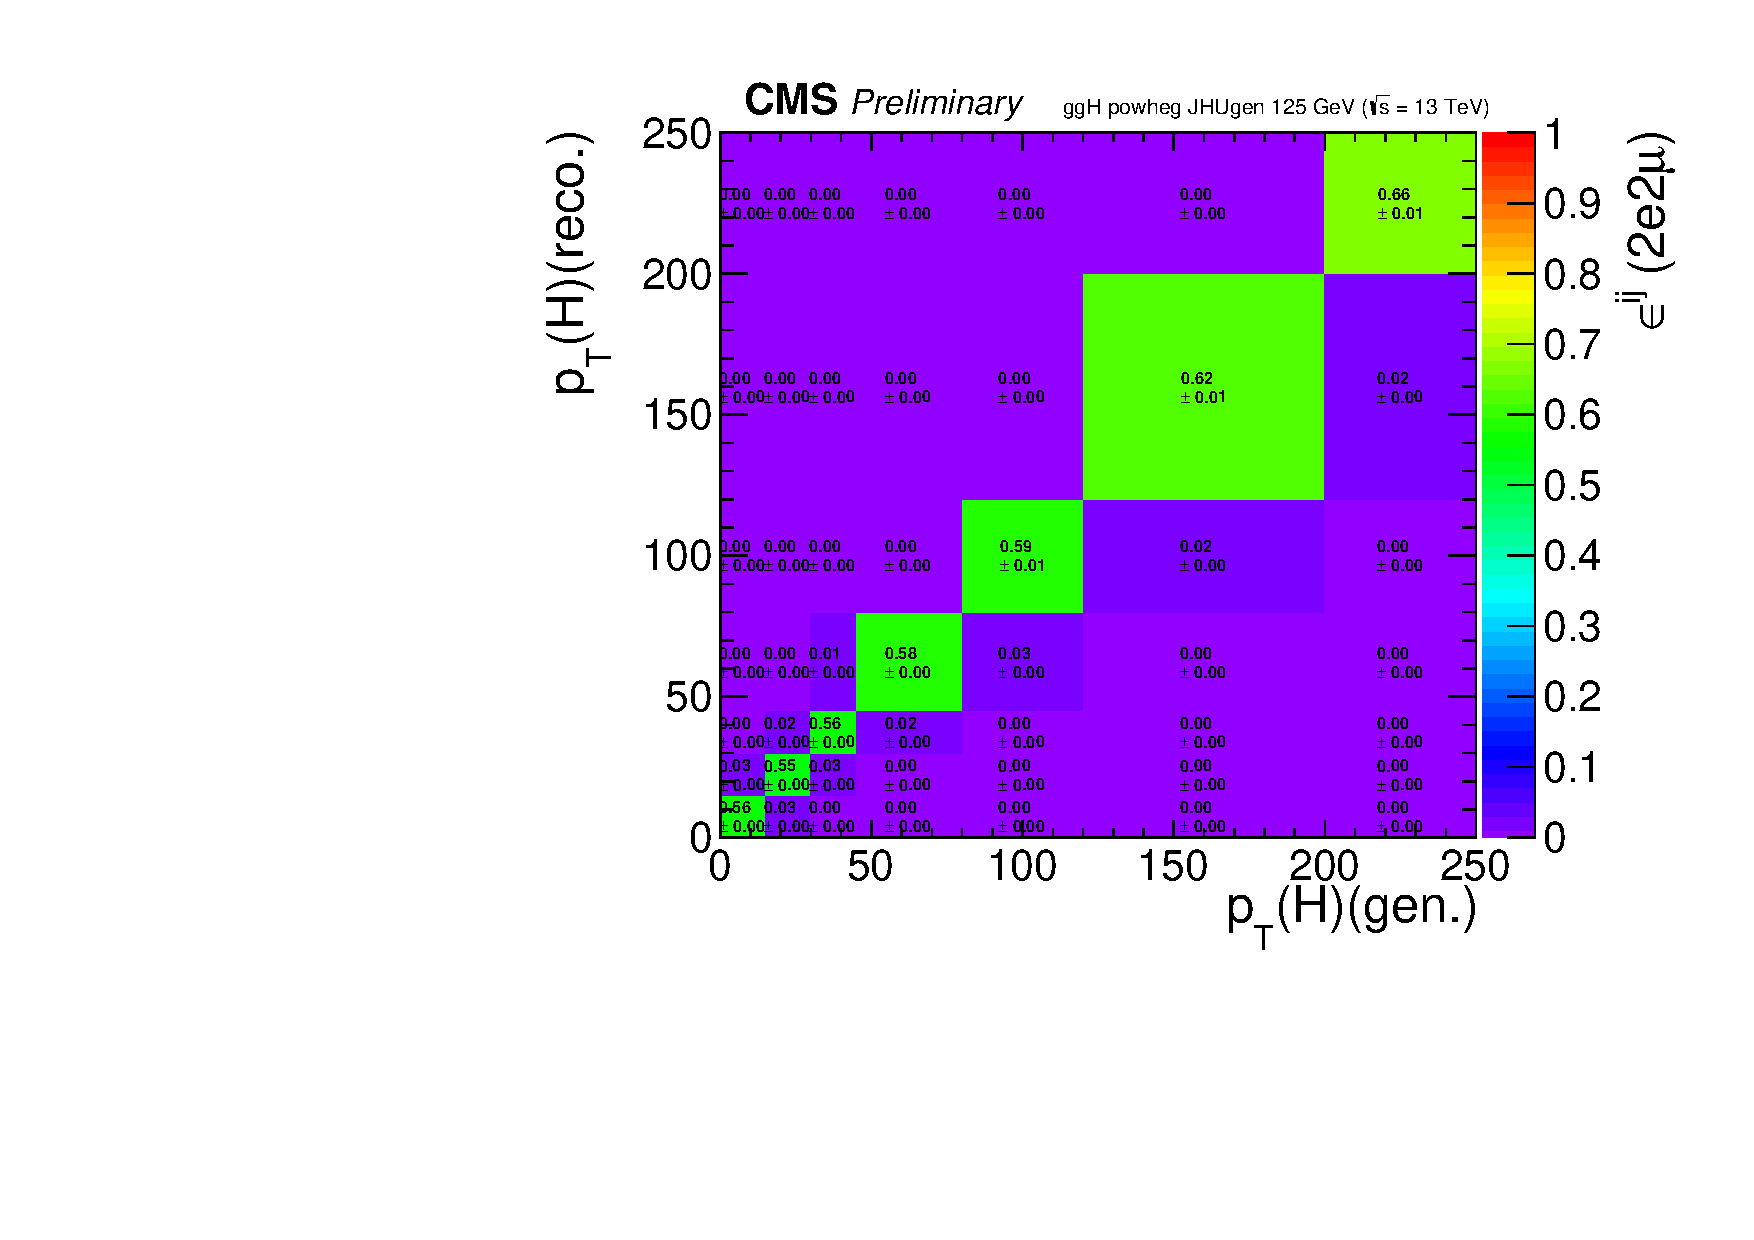
\includegraphics[width=0.32\linewidth]{Figures/results/fiducial/2018/eff2d_ggH_powheg_JHUgen_125_pT4l_2e2mu.pdf} \\
%	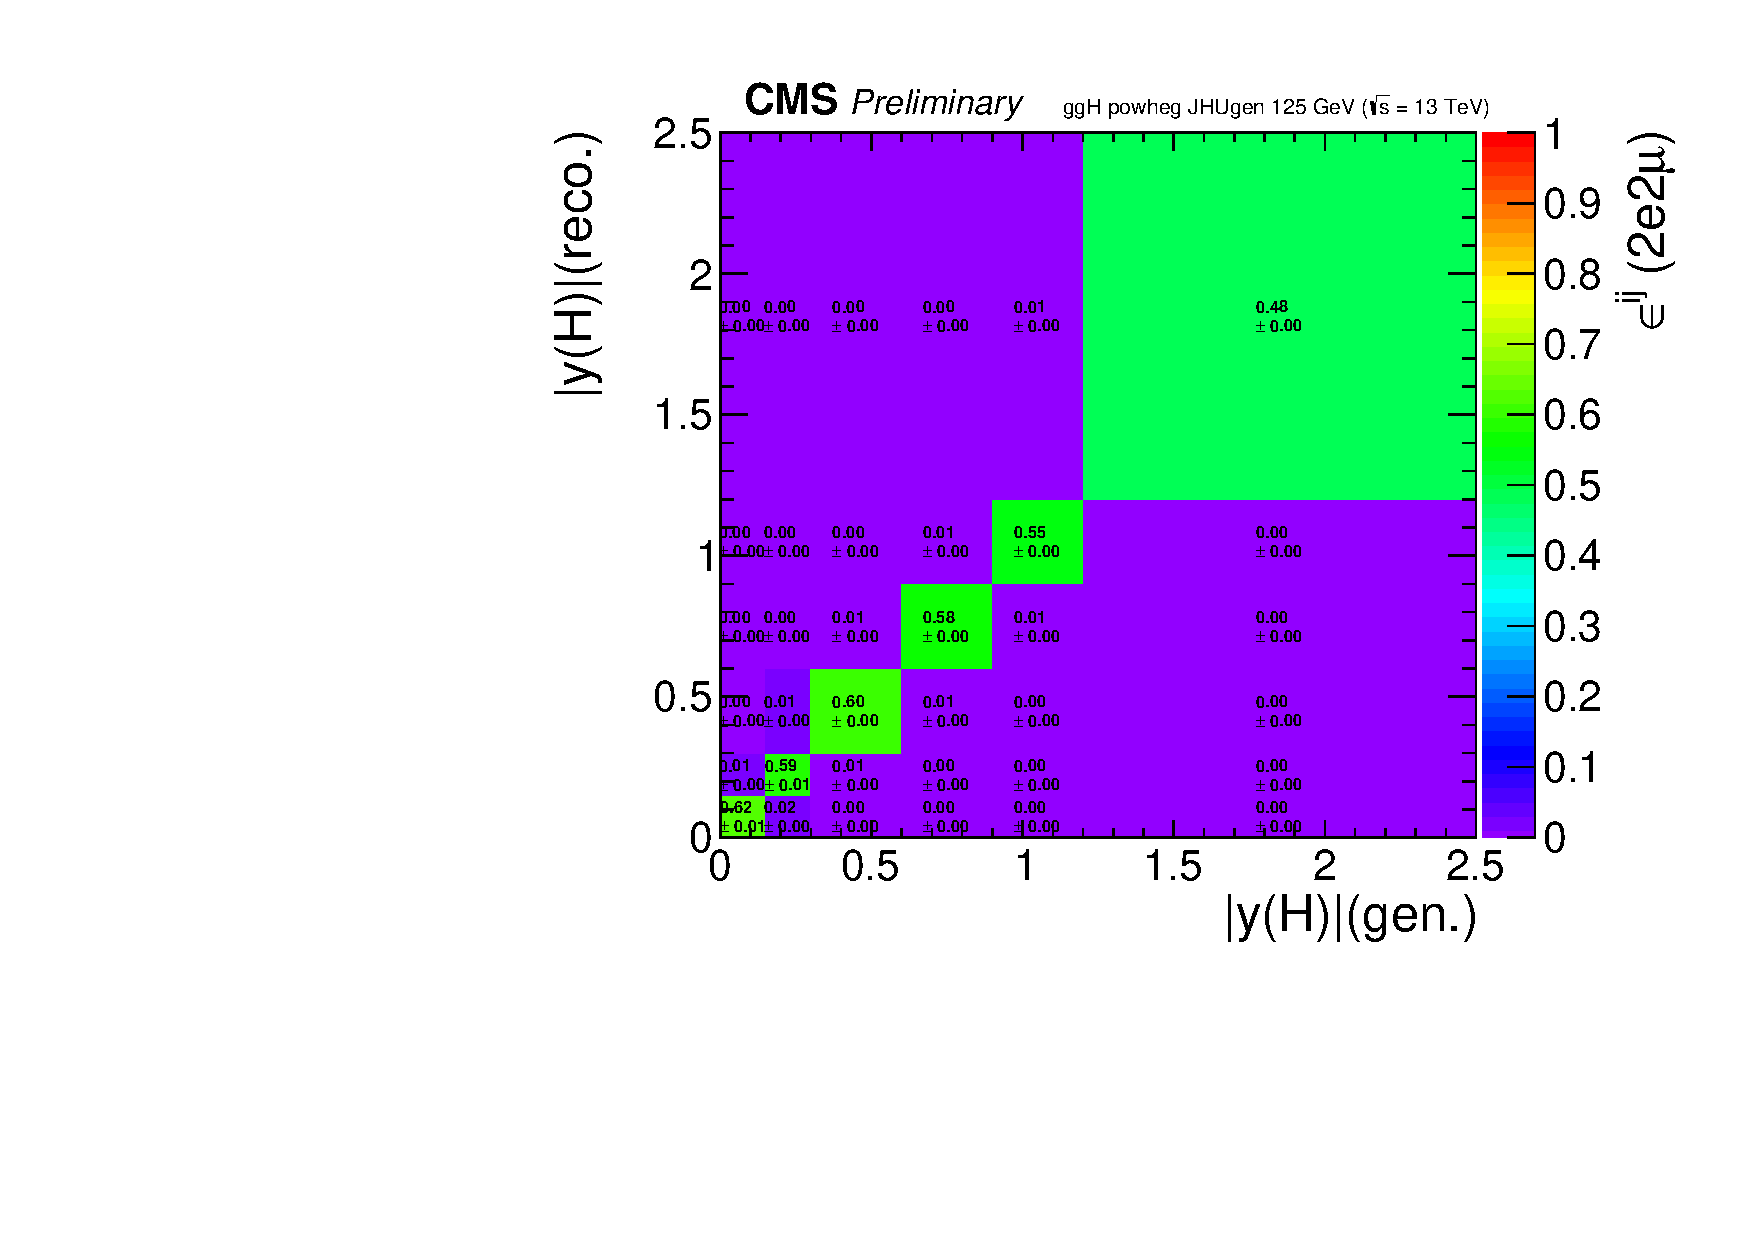
\includegraphics[width=0.32\linewidth]{Figures/results/fiducial/2016/eff2d_ggH_powheg_JHUgen_125_rapidity4l_2e2mu.pdf}
%	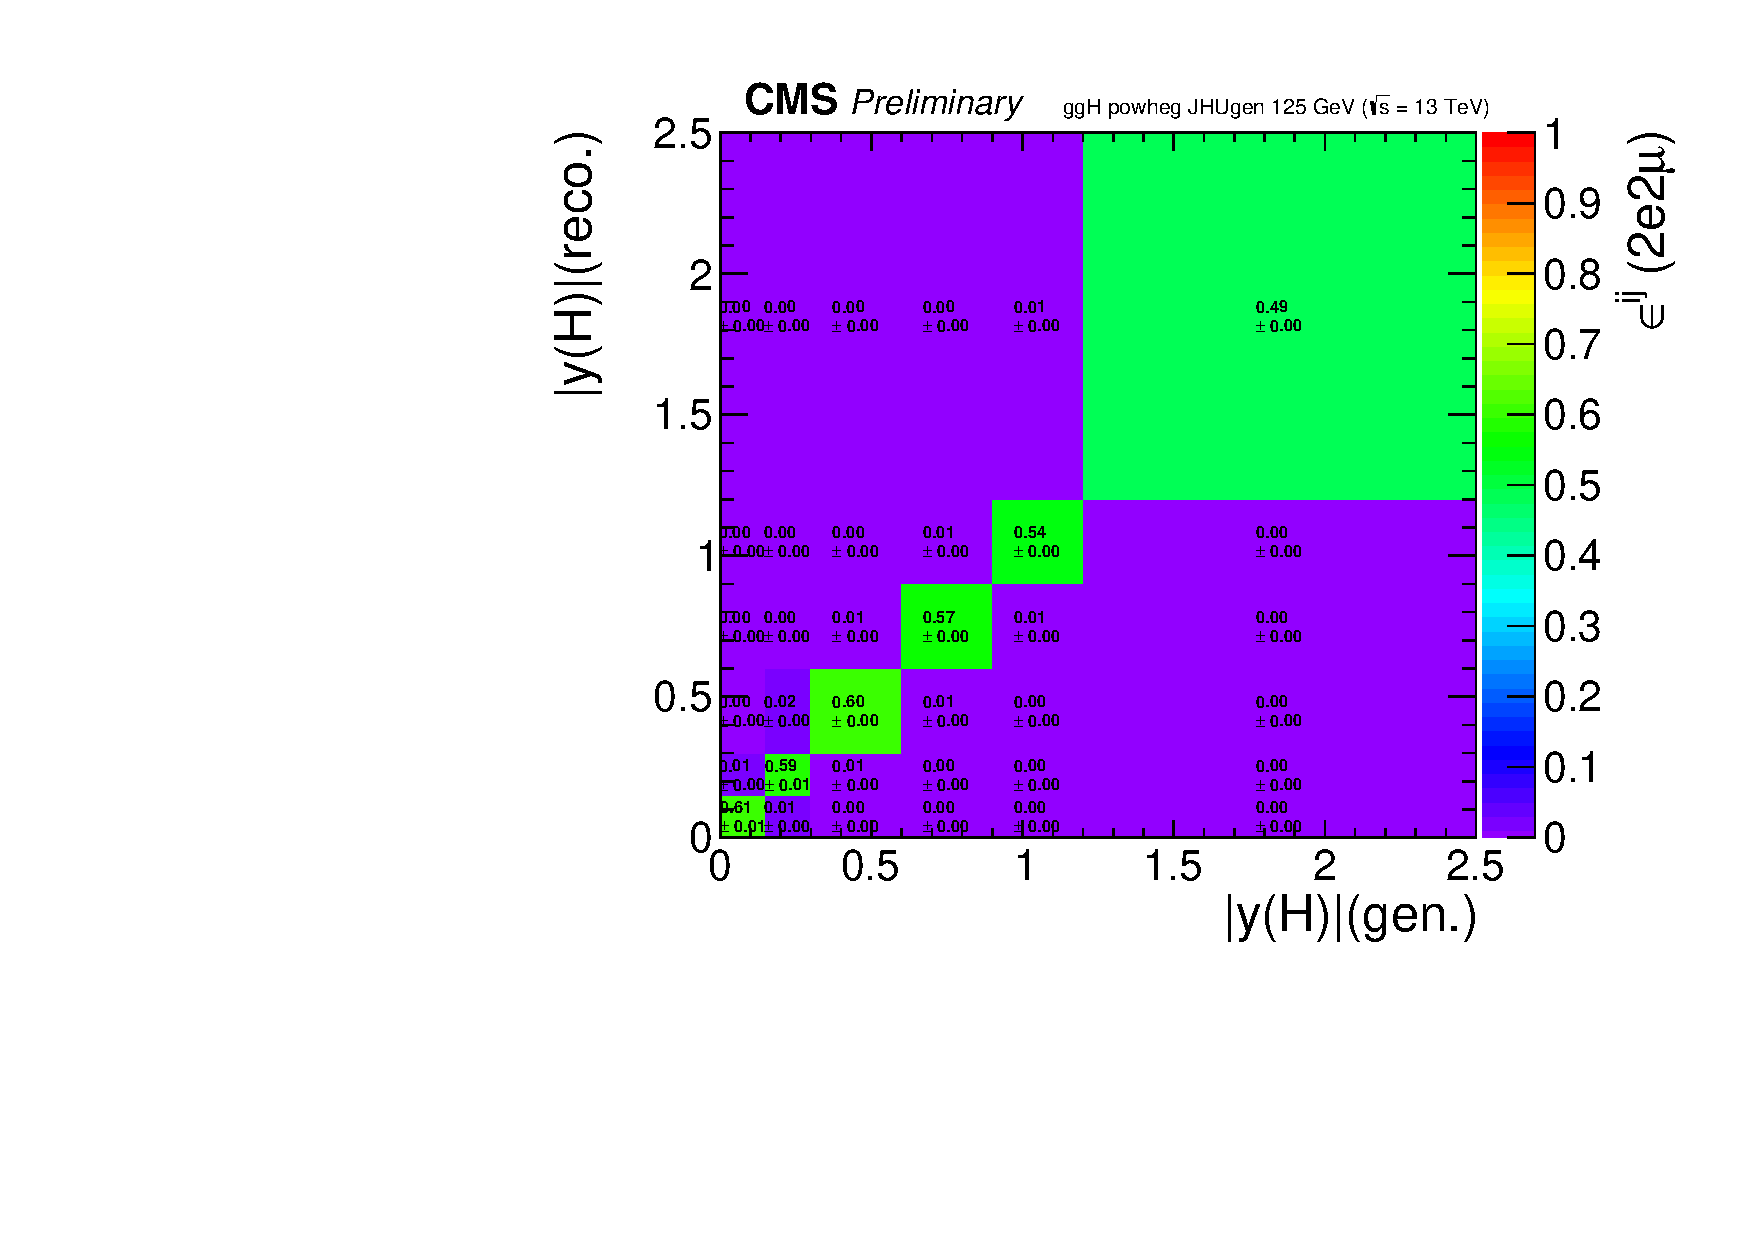
\includegraphics[width=0.32\linewidth]{Figures/results/fiducial/2017/eff2d_ggH_powheg_JHUgen_125_rapidity4l_2e2mu.pdf}
%	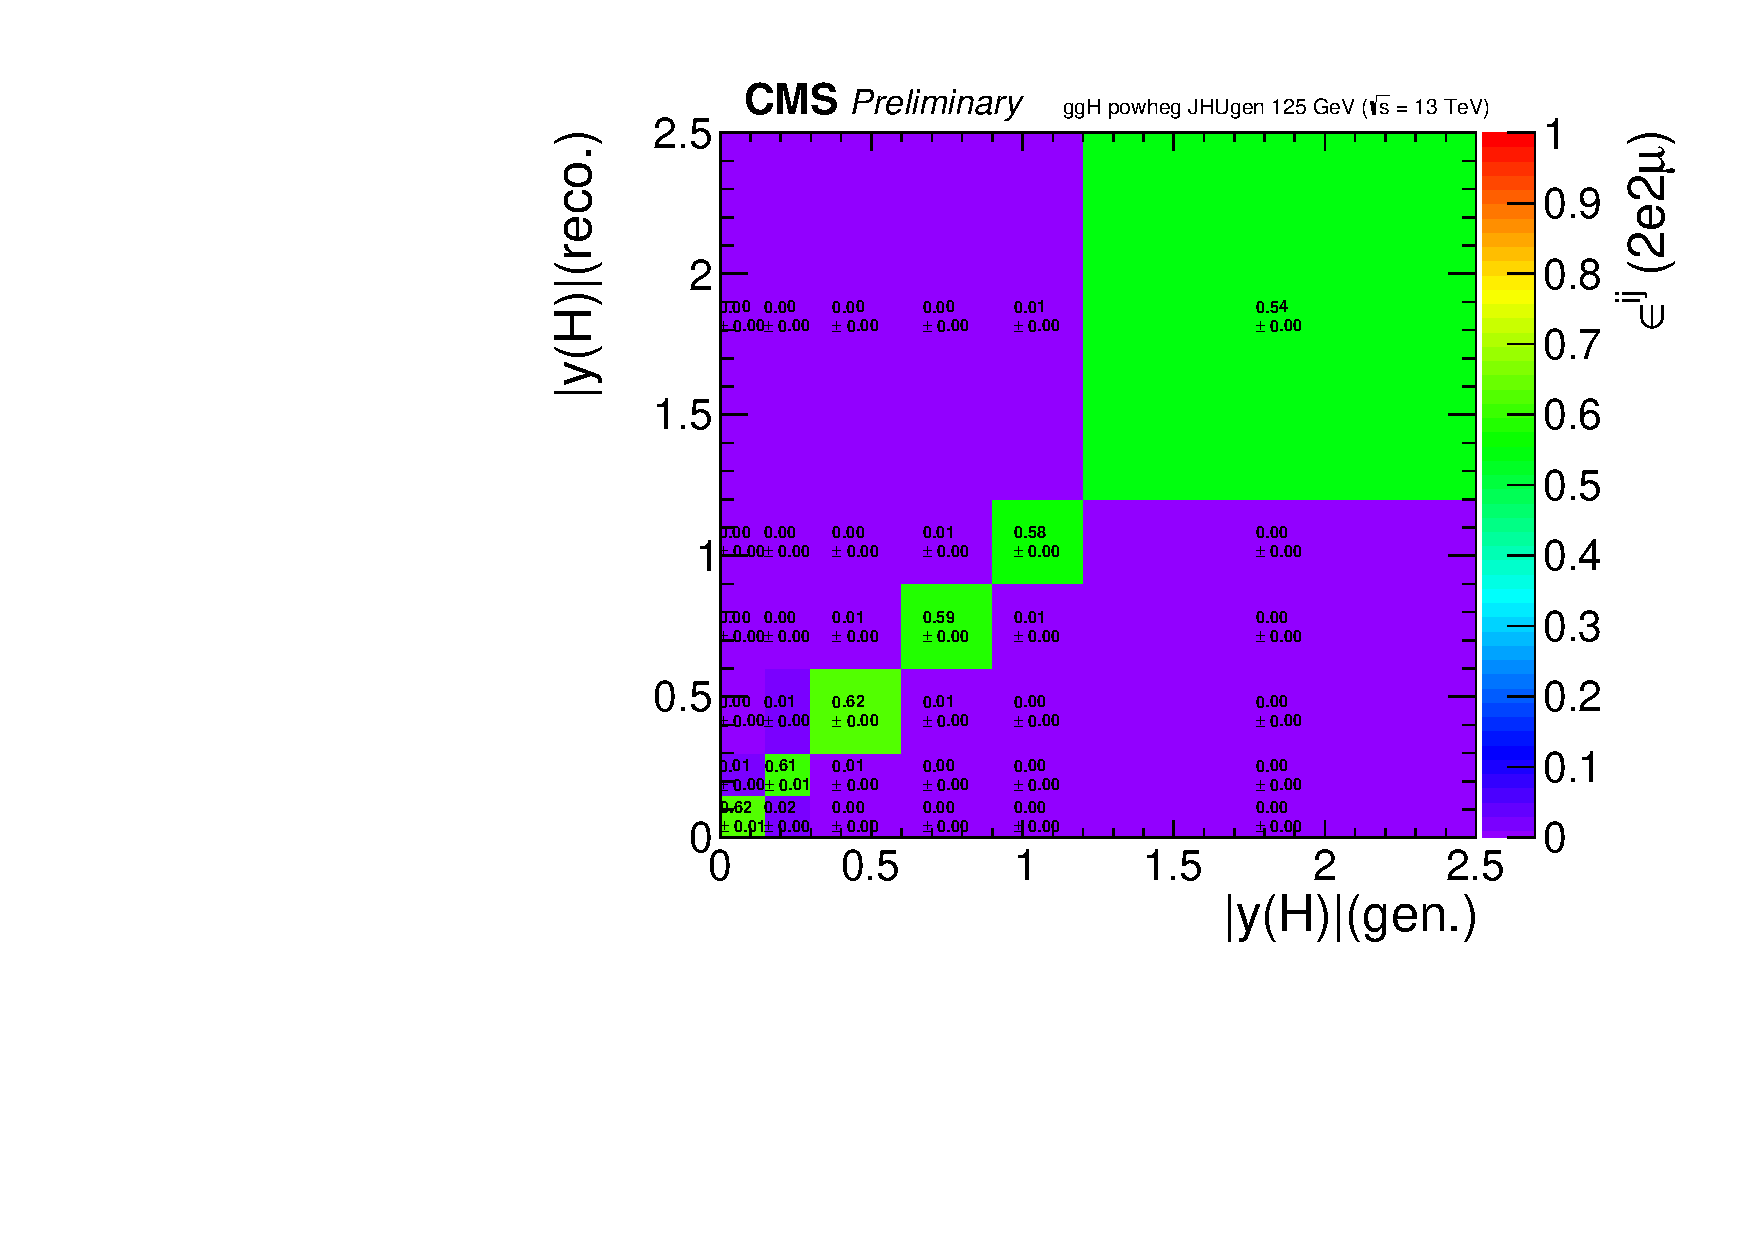
\includegraphics[width=0.32\linewidth]{Figures/results/fiducial/2018/eff2d_ggH_powheg_JHUgen_125_rapidity4l_2e2mu.pdf} \\
%	\includegraphics[width=0.32\linewidth]{Figures/results/fiducial/2016/eff2d_ggH_powheg_JHUgen_125_njets_pt30_eta2p5_2e2mu.pdf}
%	\includegraphics[width=0.32\linewidth]{Figures/results/fiducial/2017/eff2d_ggH_powheg_JHUgen_125_njets_pt30_eta2p5_2e2mu.pdf}
%	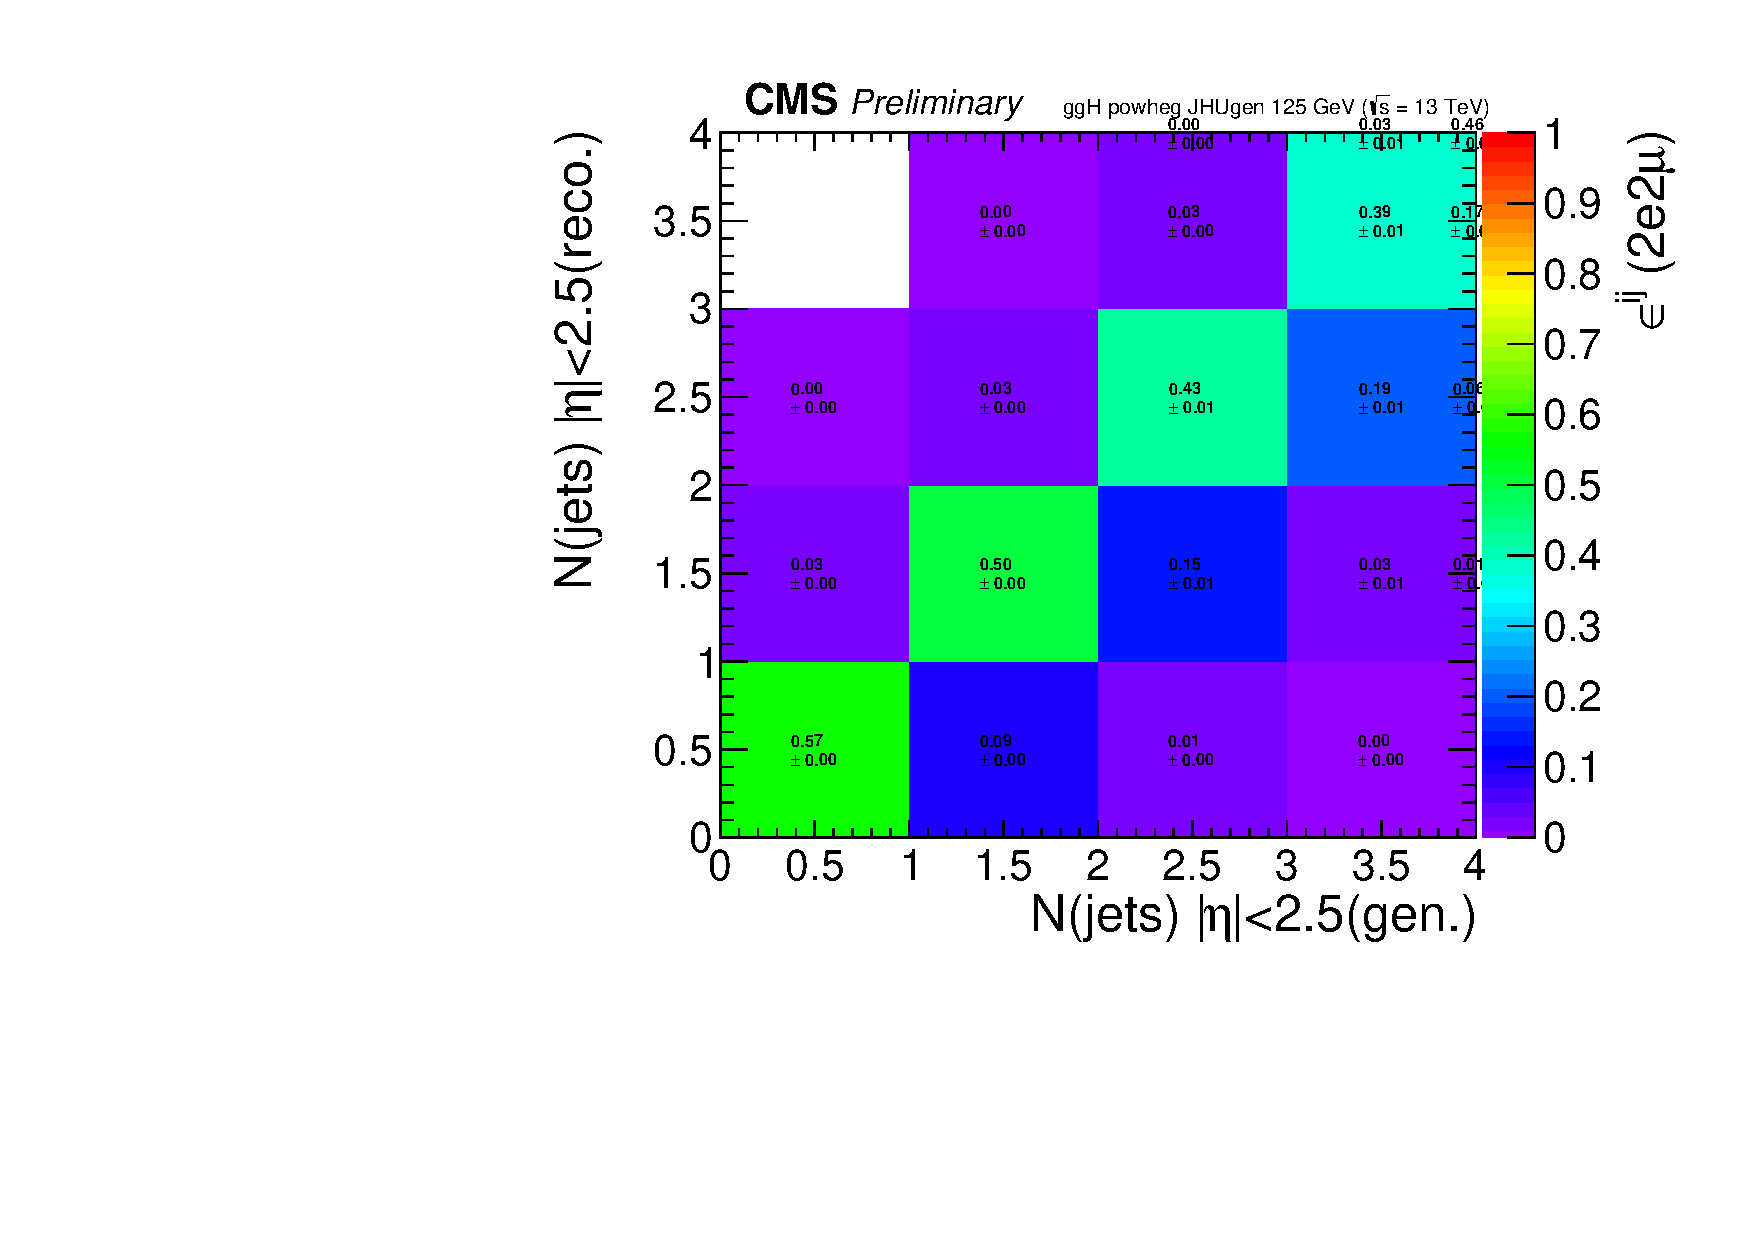
\includegraphics[width=0.32\linewidth]{Figures/results/fiducial/2018/eff2d_ggH_powheg_JHUgen_125_njets_pt30_eta2p5_2e2mu.pdf} 
%	
%	\caption{Efficiency matrices for the $\pt_{\rm H}$ (top) and $y{\rm H}$ (middle) and N(jets) (bottom) observables for gluon fusion production
%		modes in the $2e2\mu$ final state in 2016 (left) 2017 (middle) and 2018 (right). \label{fig:eff2d}}
%\end{figure}
%
%
%\subsubsubsection{Measurement results}
%
%The result of the simultaneous fit to to the $\mllll$ spectrum is shown for each final state in Fig.~\ref{fig:fiducialfit}. The fiducial cross subsection using this defintion is measured to be:
%
%\begin{eqnarray}
%\label{eqn:fidresult}
%2.85^{+0.24}_{-0.23}({\rm stat.})^{+0.15}_{-0.14}({\rm sys.})~{\rm fb}
%\end{eqnarray}
%
%This can be compared to the SM expectation of $\sigma_{{\rm fid.}}^{\rm SM}=2.72\pm0.14~{\rm fb}$.
%
%\begin{figure}[!h]
%	\centering
%	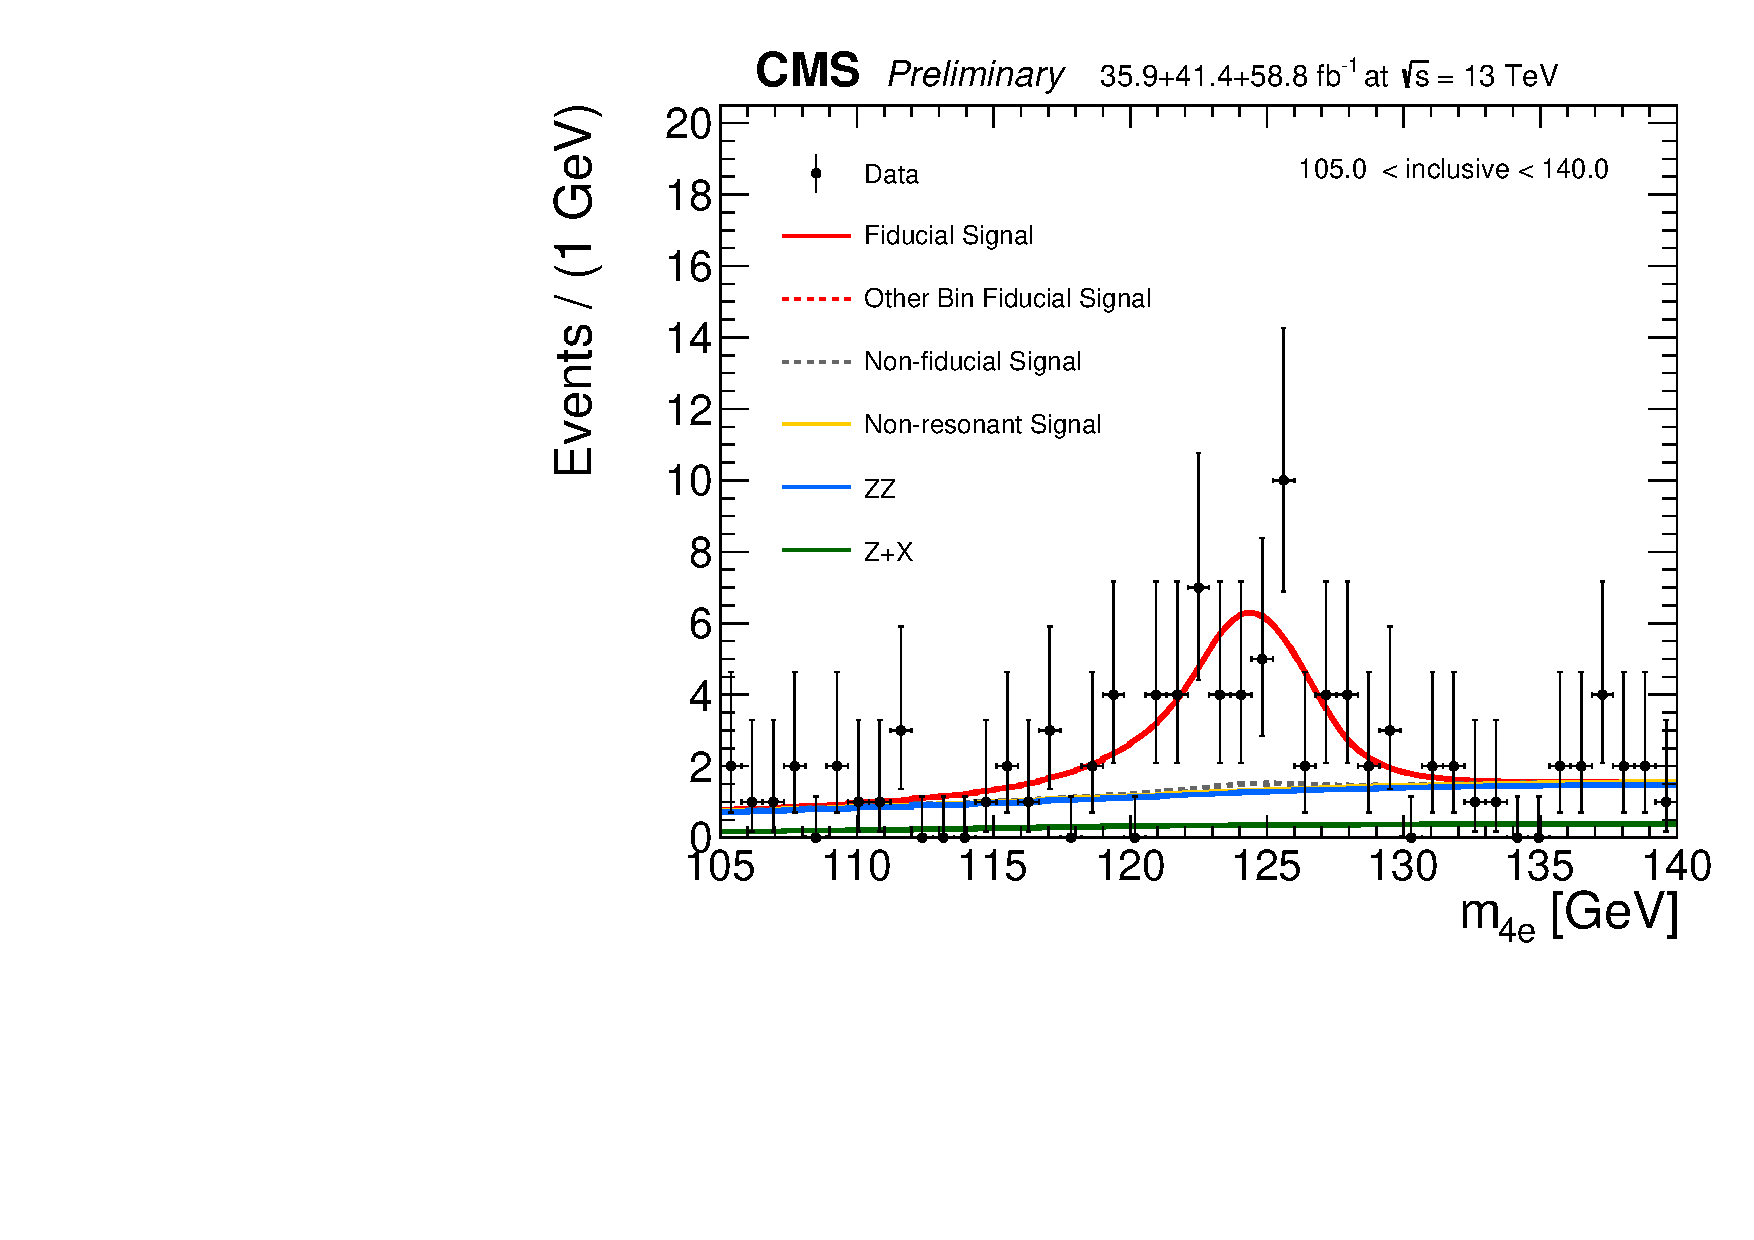
\includegraphics[width=0.45\linewidth]{Figures/results/fiducial/comb/unblind_Feb25/data_unfoldwith_SM_125_v3_mass4l_4e_recobin0.pdf}
%	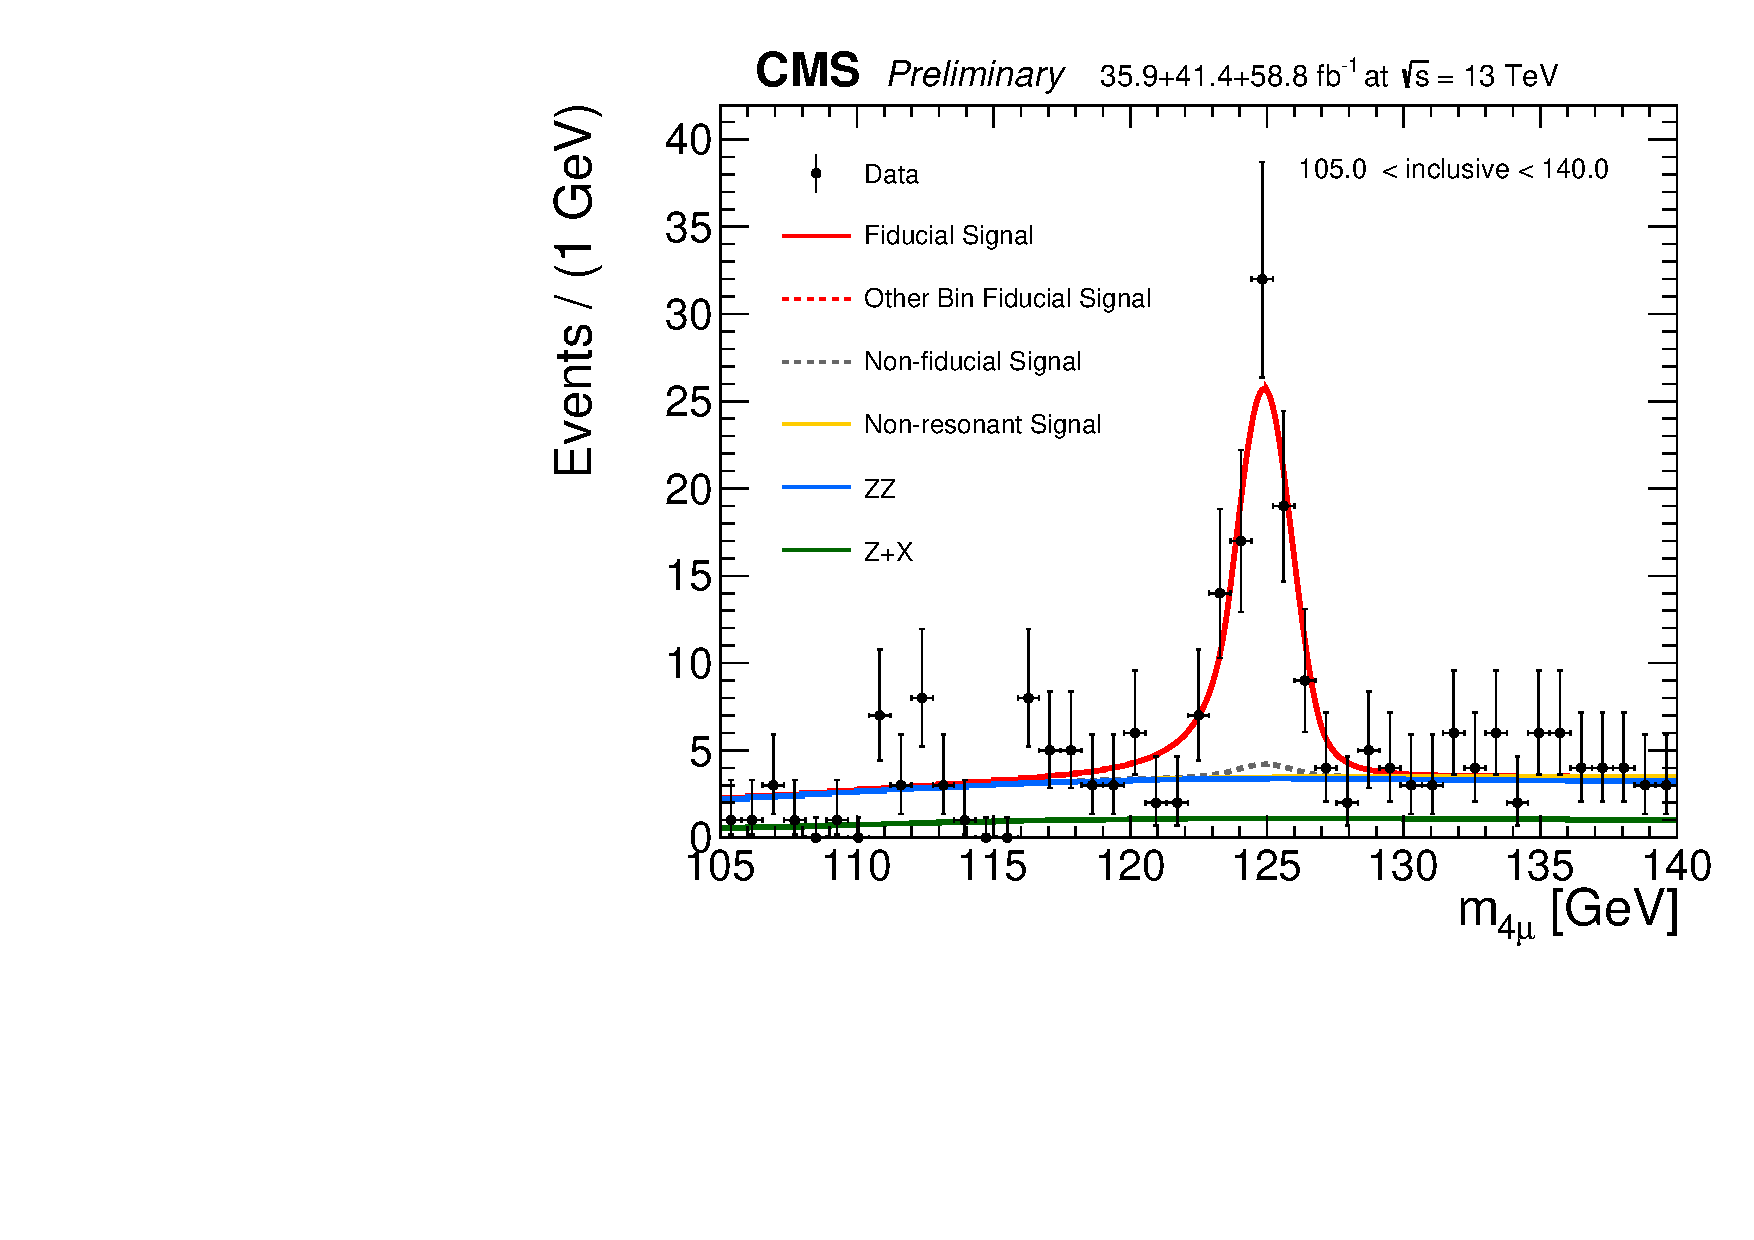
\includegraphics[width=0.45\linewidth]{Figures/results/fiducial/comb/unblind_Feb25/data_unfoldwith_SM_125_v3_mass4l_4mu_recobin0.pdf} \\
%	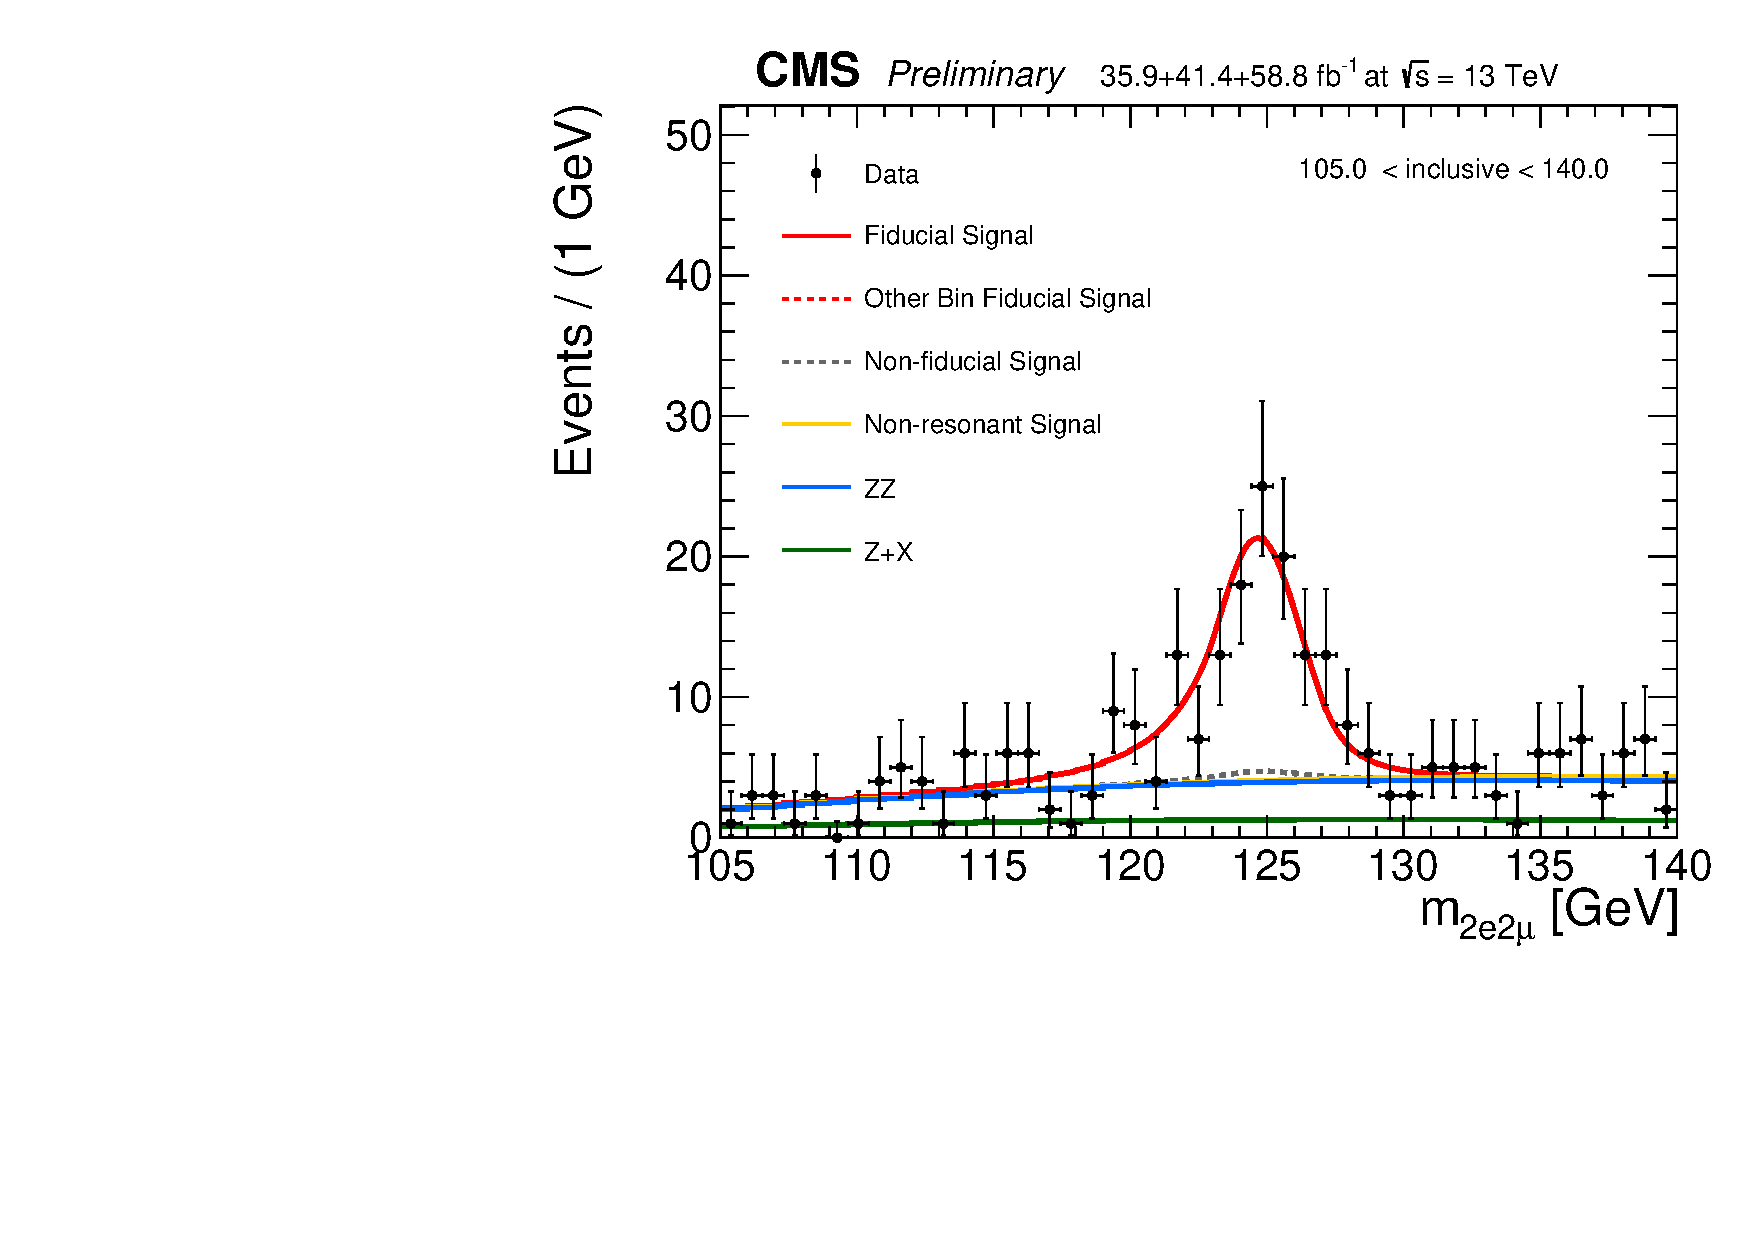
\includegraphics[width=0.45\linewidth]{Figures/results/fiducial/comb/unblind_Feb25/data_unfoldwith_SM_125_v3_mass4l_2e2mu_recobin0.pdf} 
%	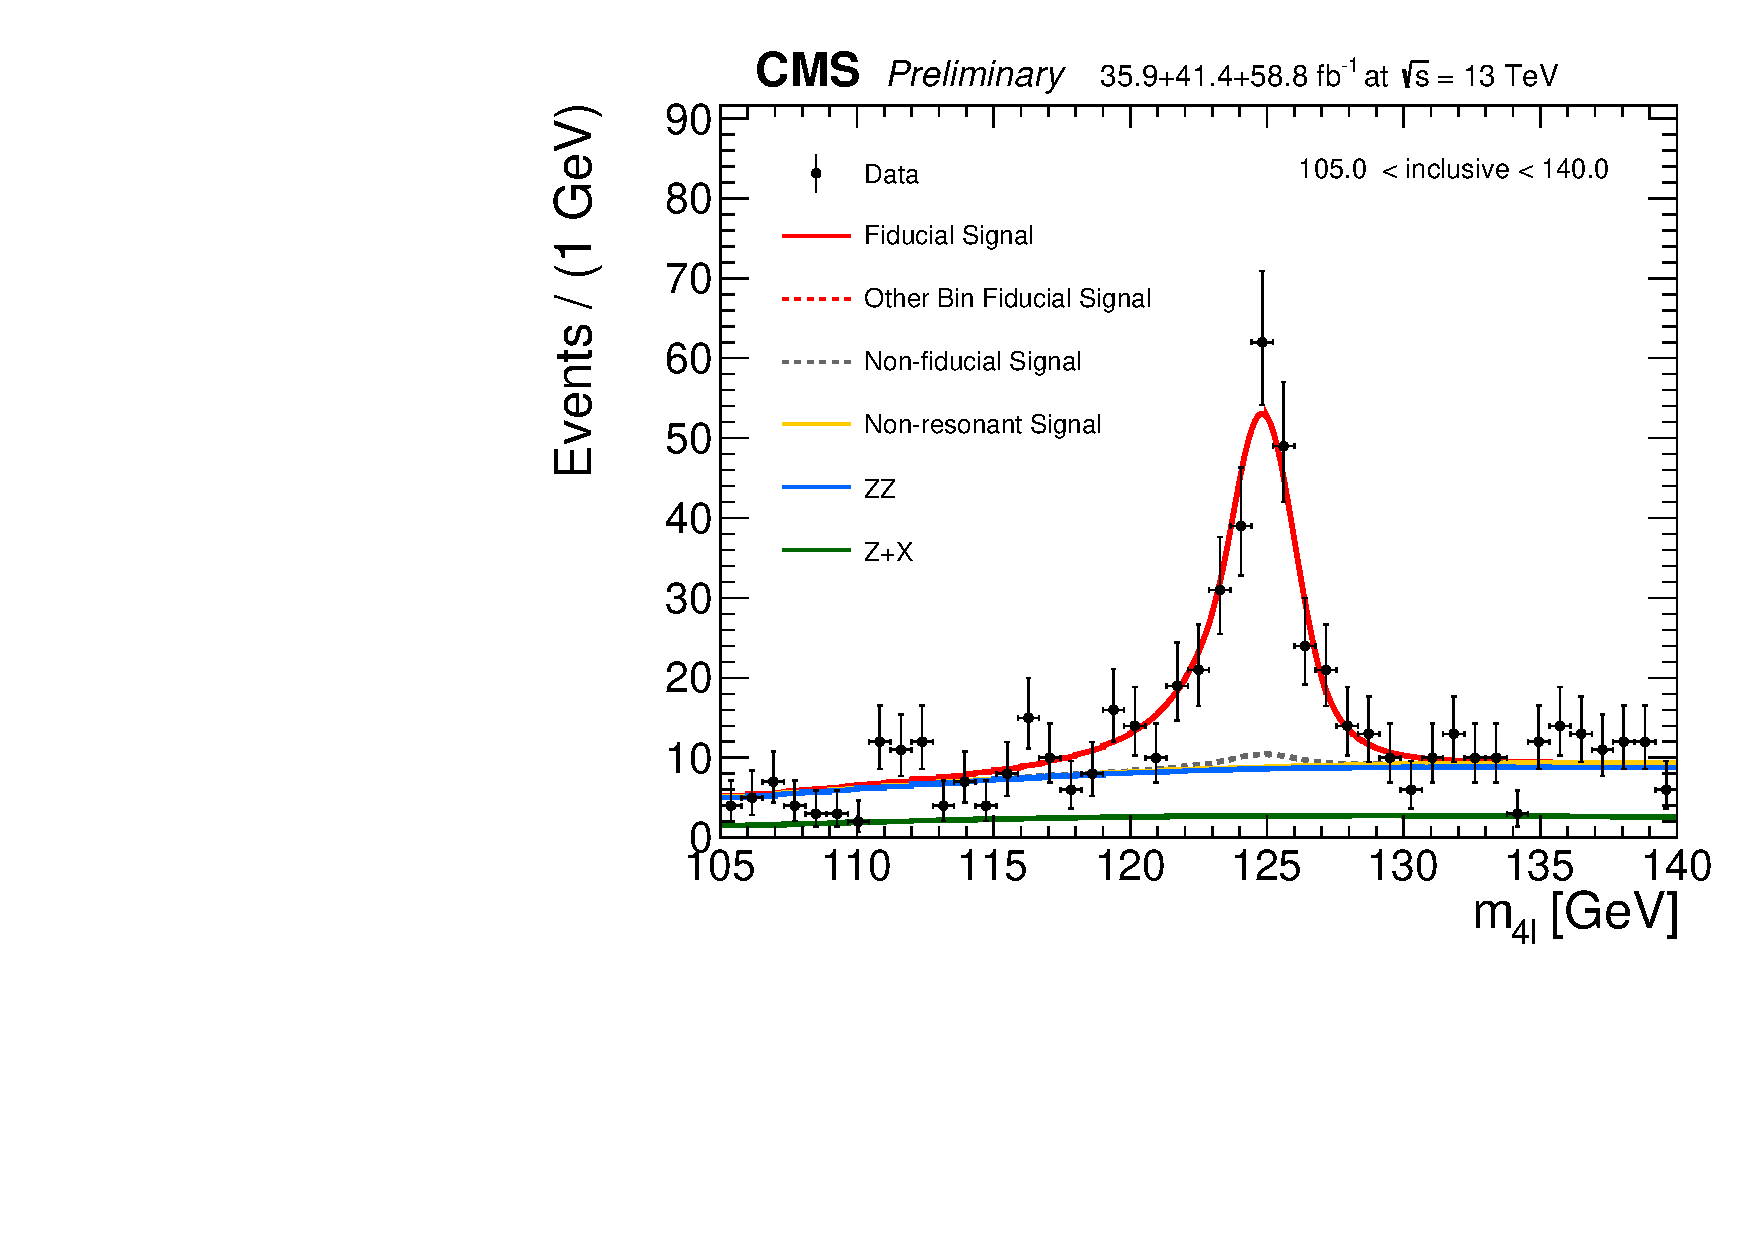
\includegraphics[width=0.45\linewidth]{Figures/results/fiducial/comb/unblind_Feb25/data_unfoldwith_SM_125_v3_mass4l_4l_recobin0.pdf} 
%	\caption{Result of simultaneous fit for the integrated fiducial cross subsection measurement in each final state. The results are shown for 2018 only. \label{fig:fiducialfit}}
%\end{figure}
%
%\begin{figure}[!h]
%	\centering
%	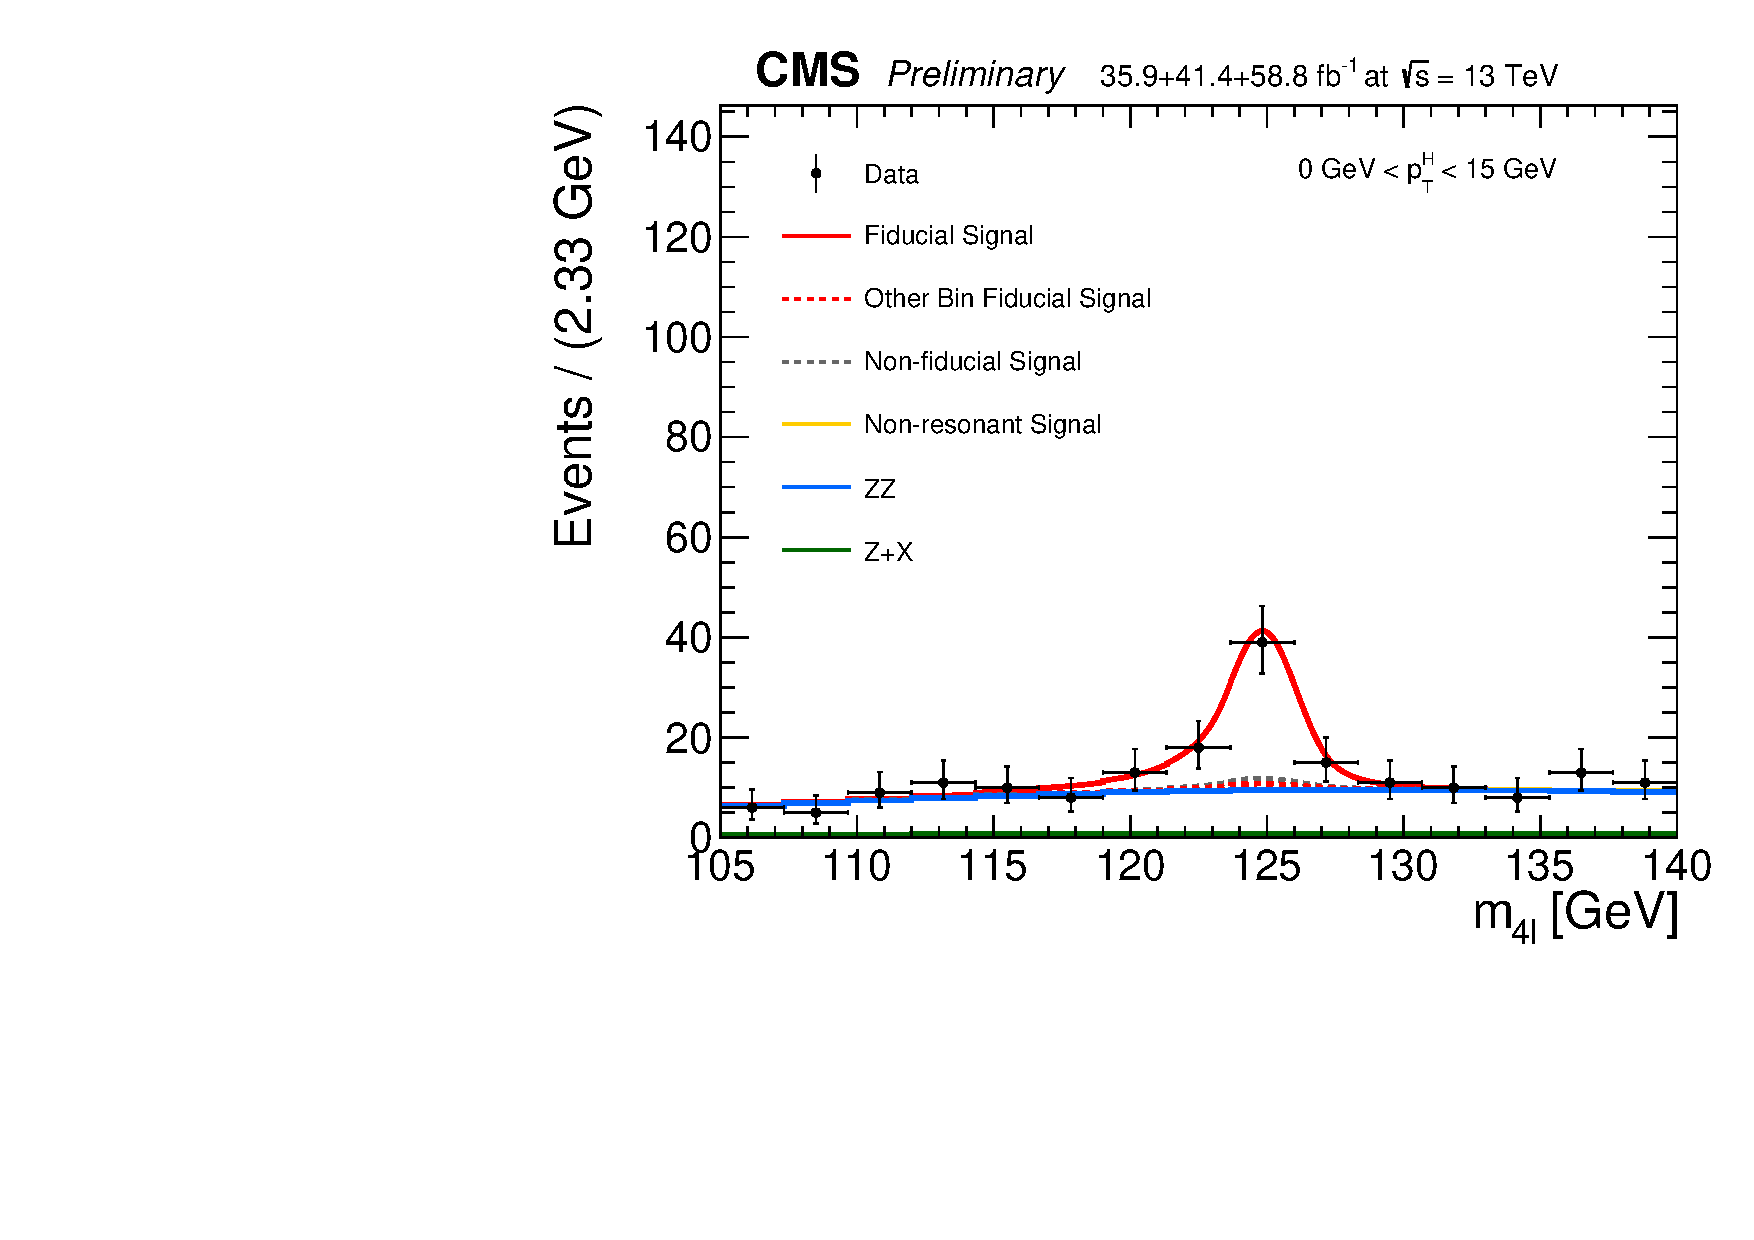
\includegraphics[width=0.32\linewidth]{Figures/results/fiducial/comb/unblind_Feb25/data_unfoldwith_SM_125_v3_pT4l_4l_recobin0.pdf}
%	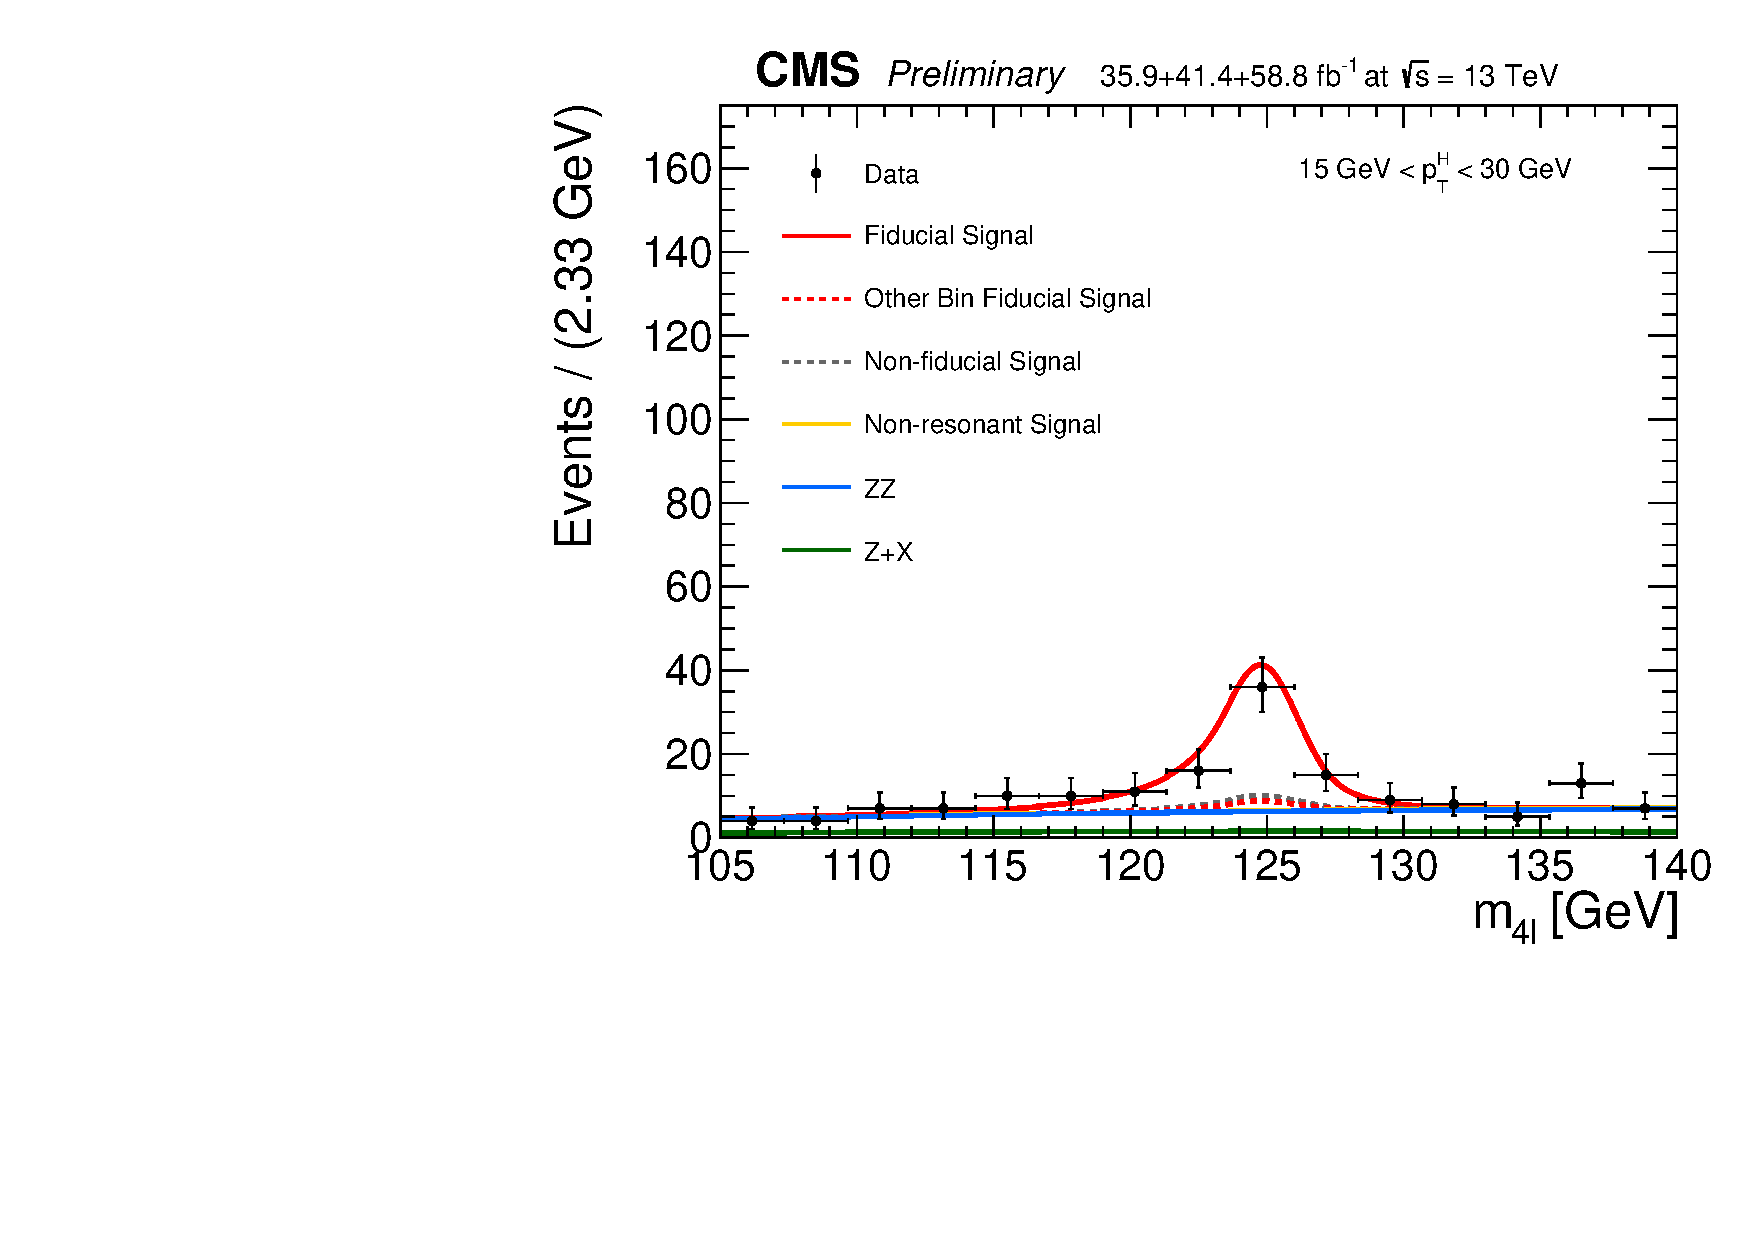
\includegraphics[width=0.32\linewidth]{Figures/results/fiducial/comb/unblind_Feb25/data_unfoldwith_SM_125_v3_pT4l_4l_recobin1.pdf}
%	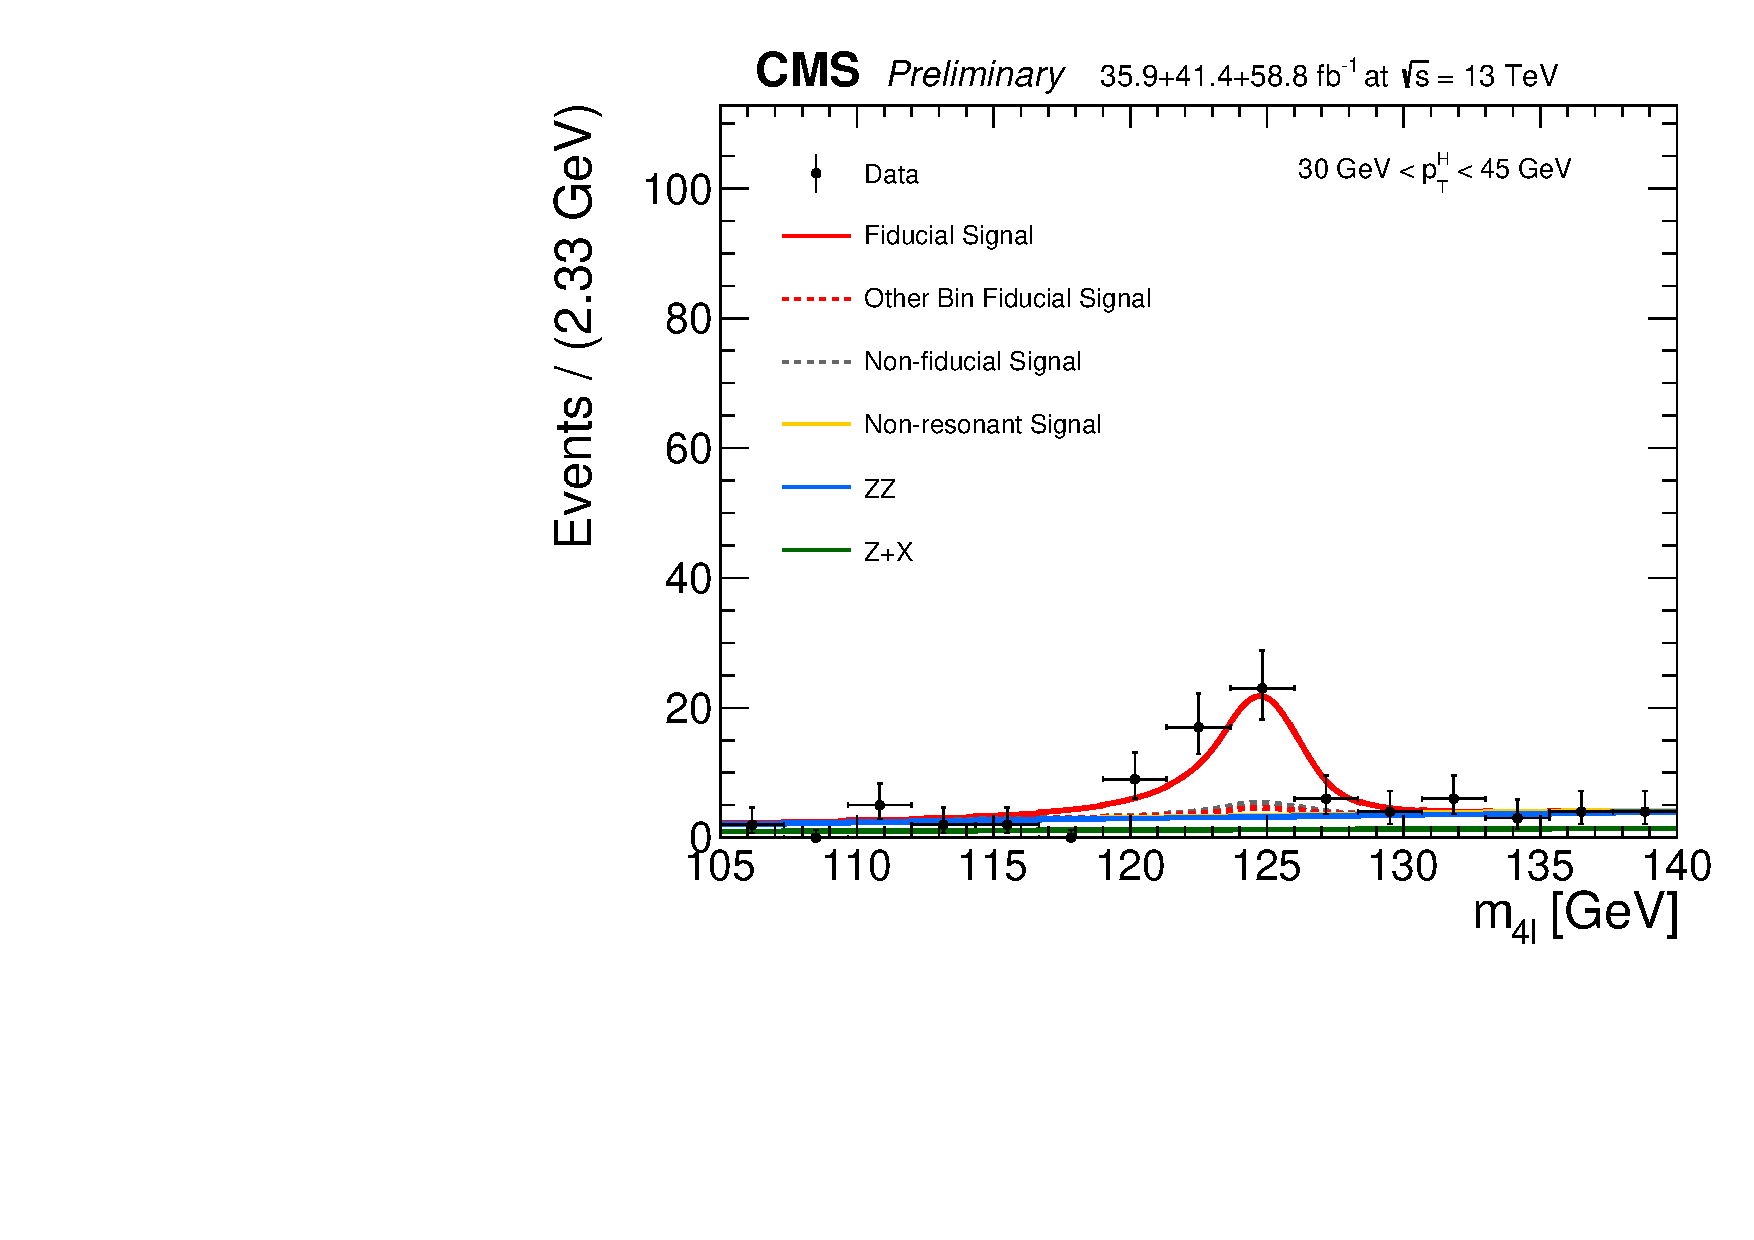
\includegraphics[width=0.32\linewidth]{Figures/results/fiducial/comb/unblind_Feb25/data_unfoldwith_SM_125_v3_pT4l_4l_recobin2.pdf}\\
%	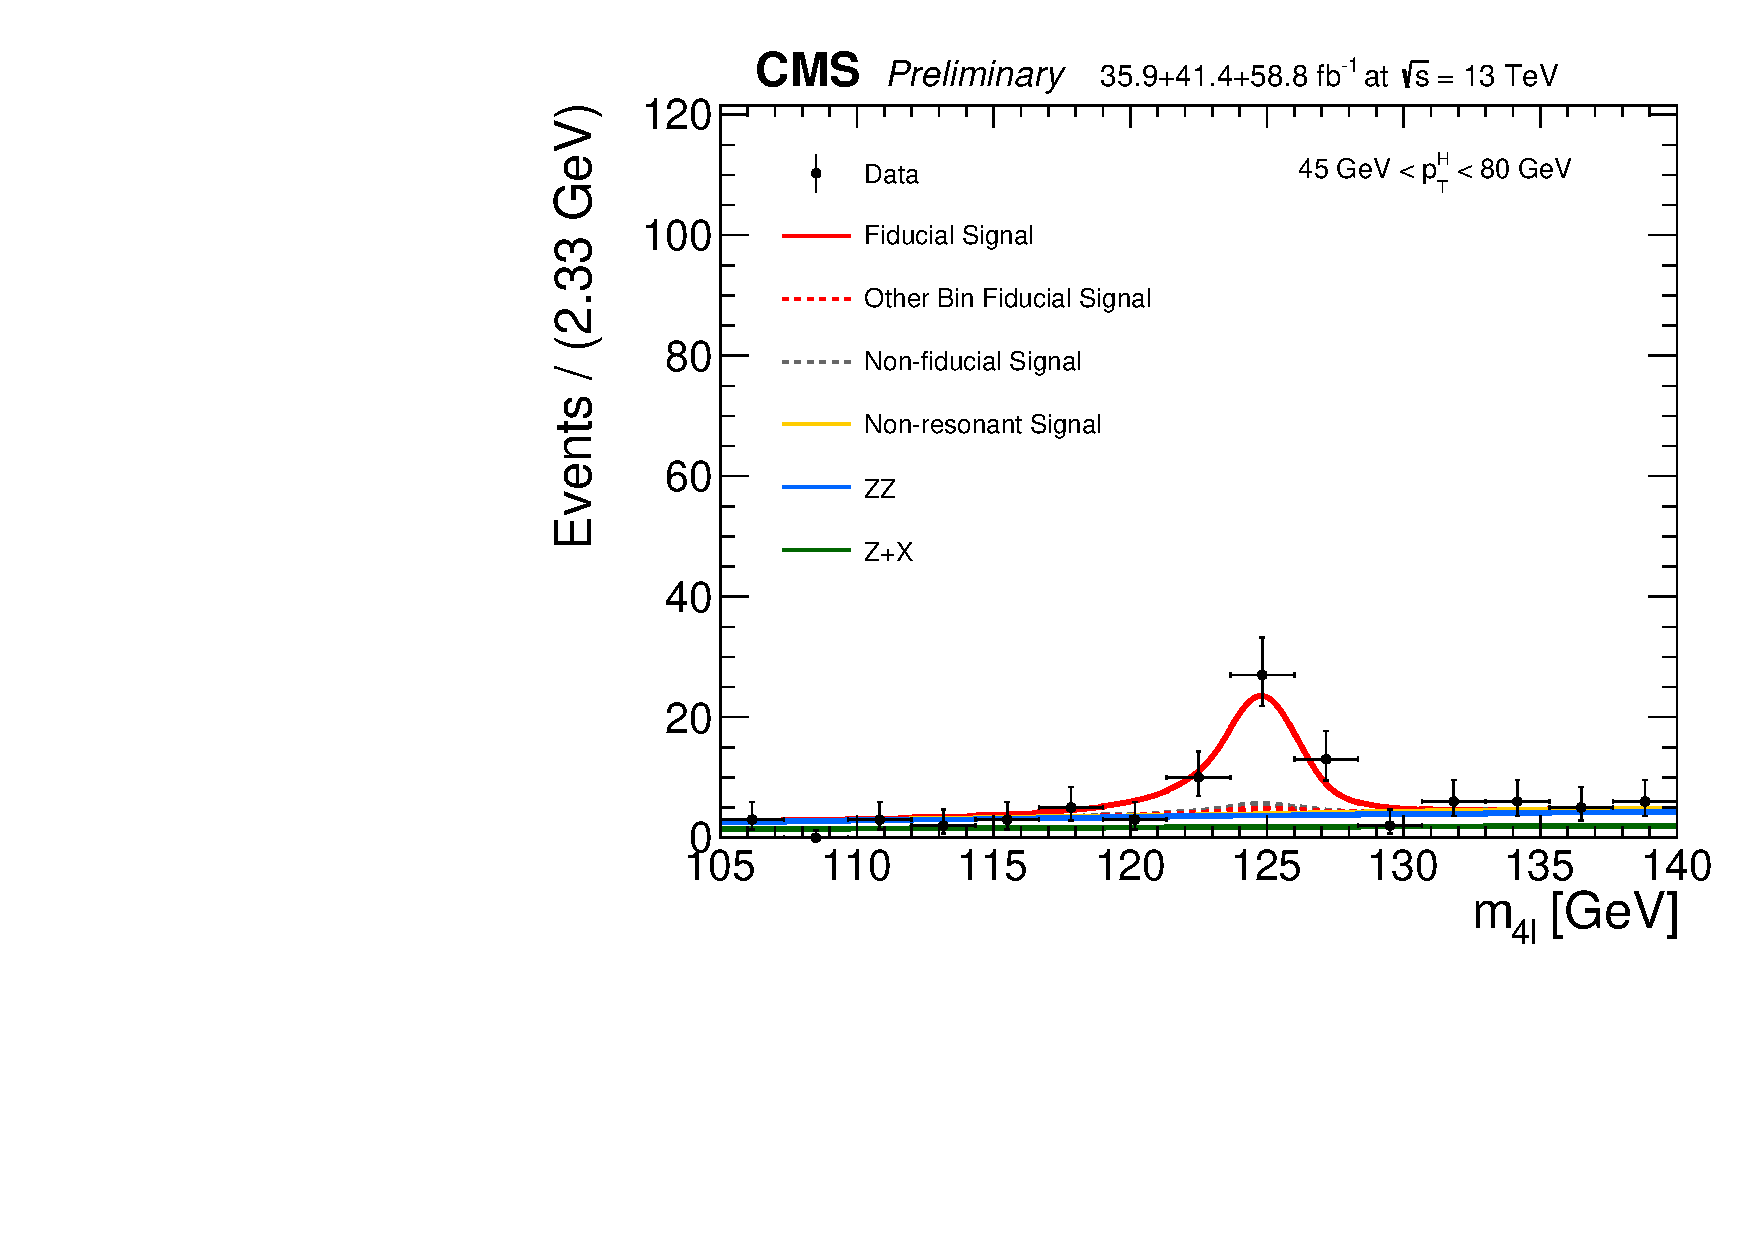
\includegraphics[width=0.32\linewidth]{Figures/results/fiducial/comb/unblind_Feb25/data_unfoldwith_SM_125_v3_pT4l_4l_recobin3.pdf}
%	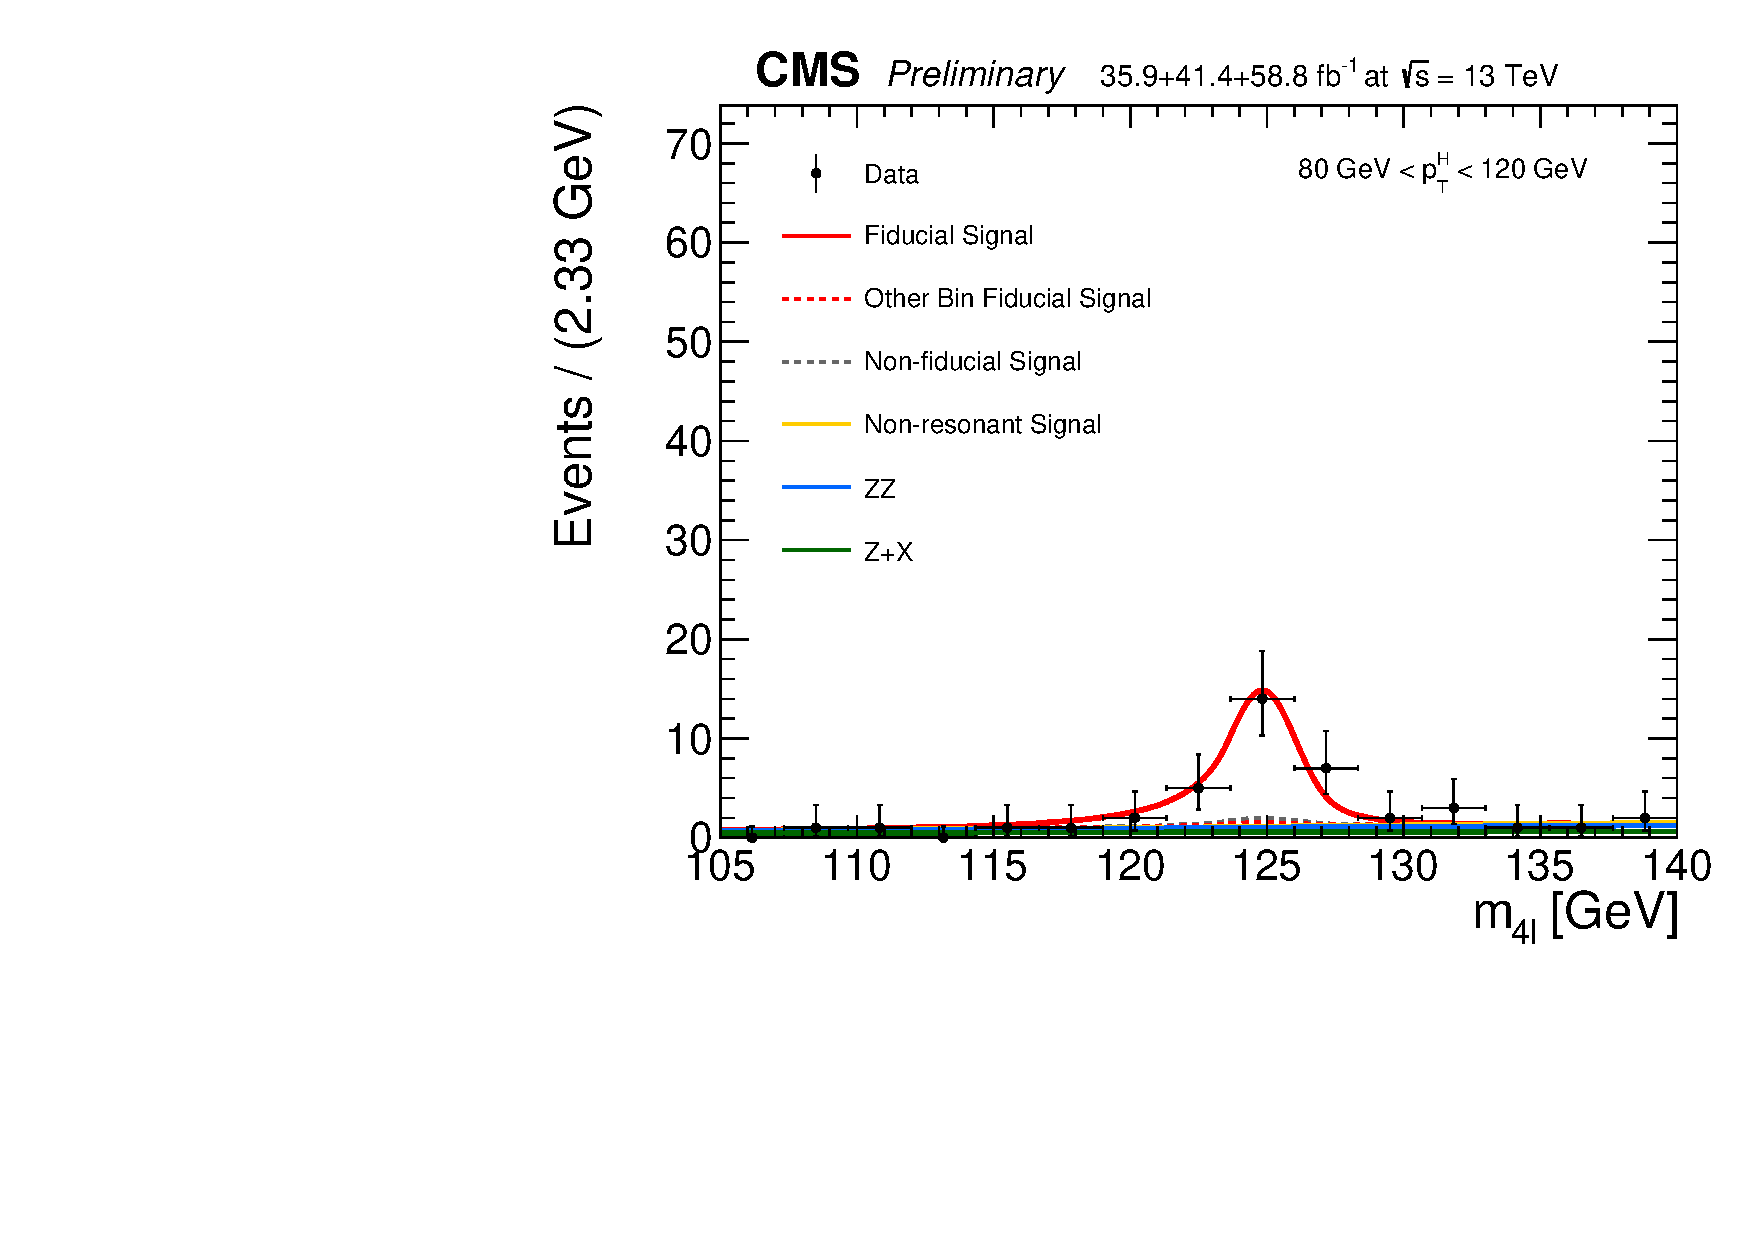
\includegraphics[width=0.32\linewidth]{Figures/results/fiducial/comb/unblind_Feb25/data_unfoldwith_SM_125_v3_pT4l_4l_recobin4.pdf}
%	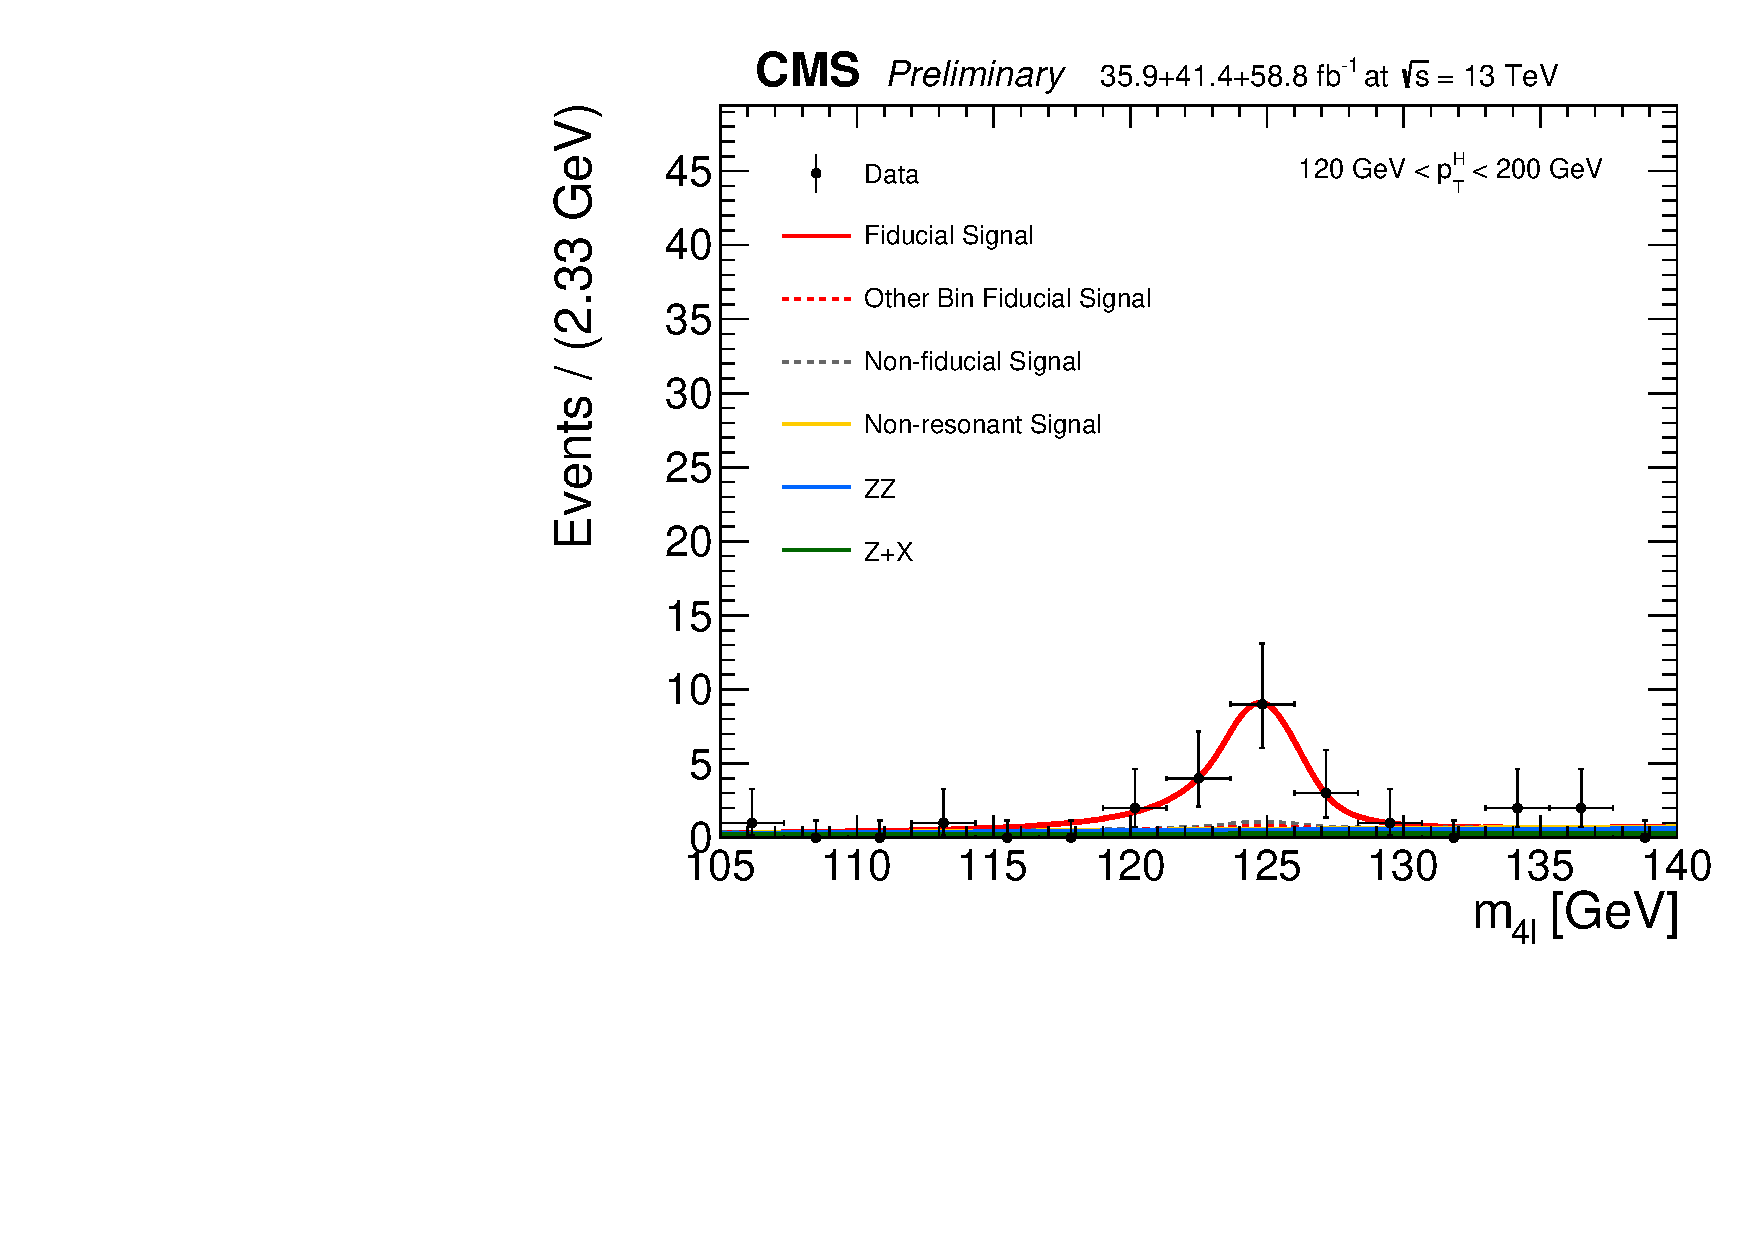
\includegraphics[width=0.32\linewidth]{Figures/results/fiducial/comb/unblind_Feb25/data_unfoldwith_SM_125_v3_pT4l_4l_recobin5.pdf} \\
%	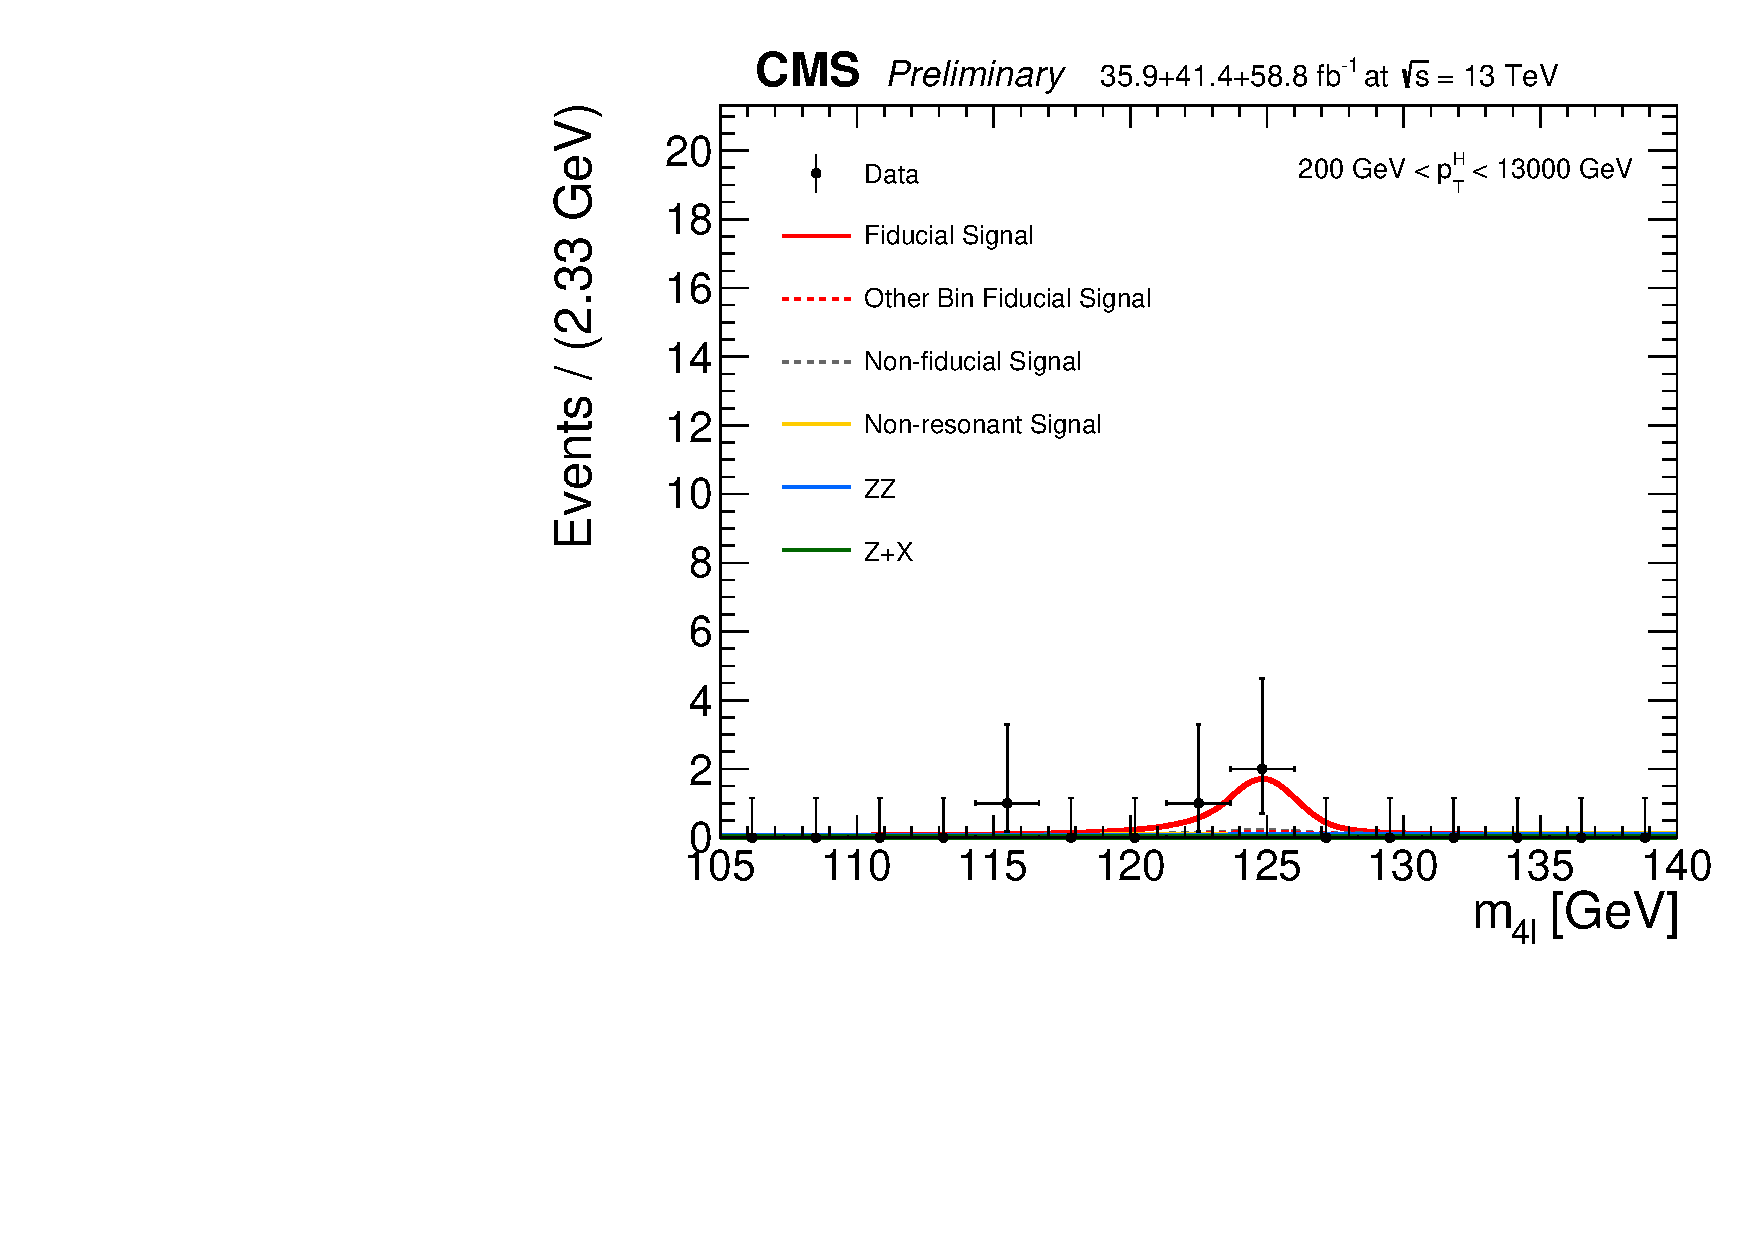
\includegraphics[width=0.32\linewidth]{Figures/results/fiducial/comb/unblind_Feb25/data_unfoldwith_SM_125_v3_pT4l_4l_recobin6.pdf}
%	\caption{Result of simultaneous fit for the differential fiducial cross subsection measurement for $\pt({\rm H})$ 
%		in each differential bin. The combined 4$\ell$ final state is shown. The results are shown for 2018 only. \label{fig:differentialfitptH}}
%\end{figure}
%
%\begin{figure}[!h]
%	\centering 
%	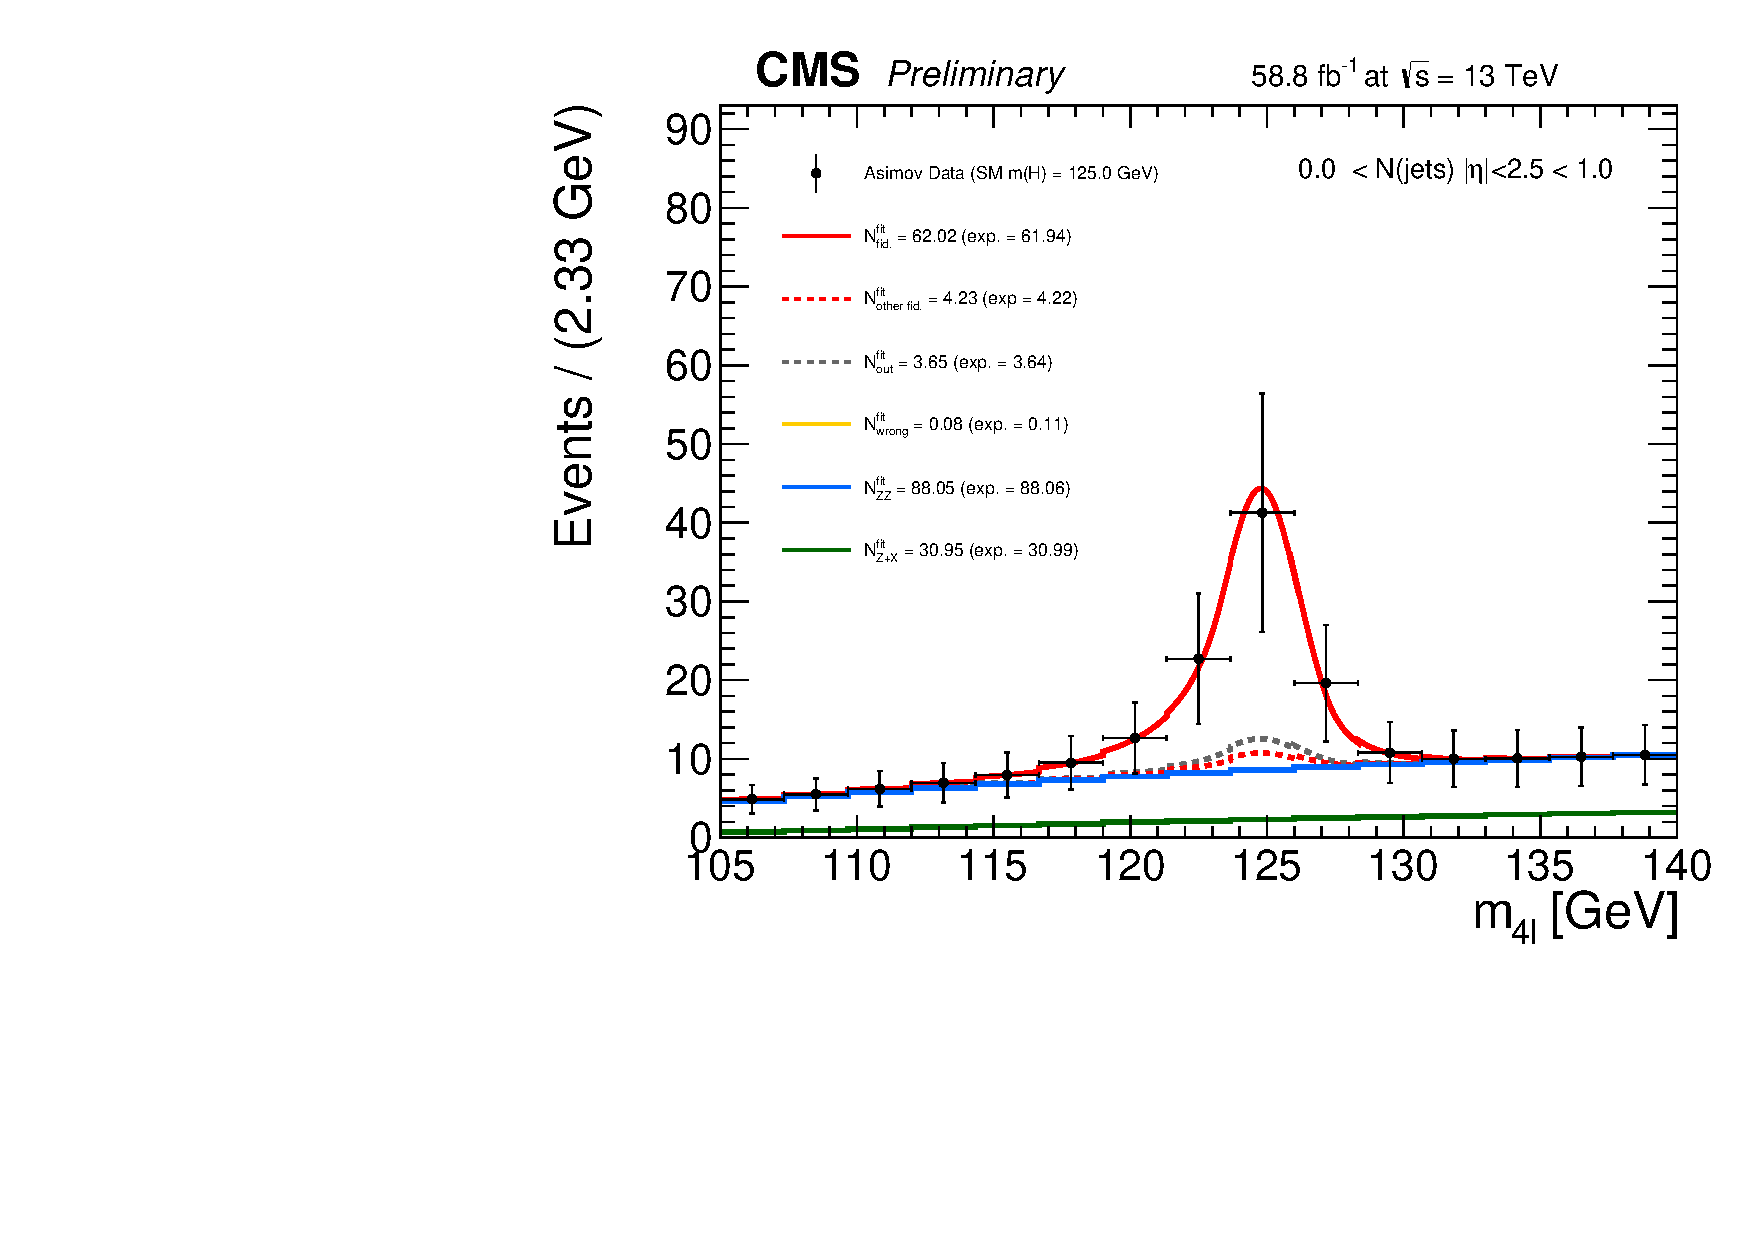
\includegraphics[width=0.32\linewidth]{Figures/results/fiducial/2018/asimovdata_SM_125_v2_unfoldwith_SM_125_v3_njets_pt30_eta2p5_4l_recobin0.pdf}
%	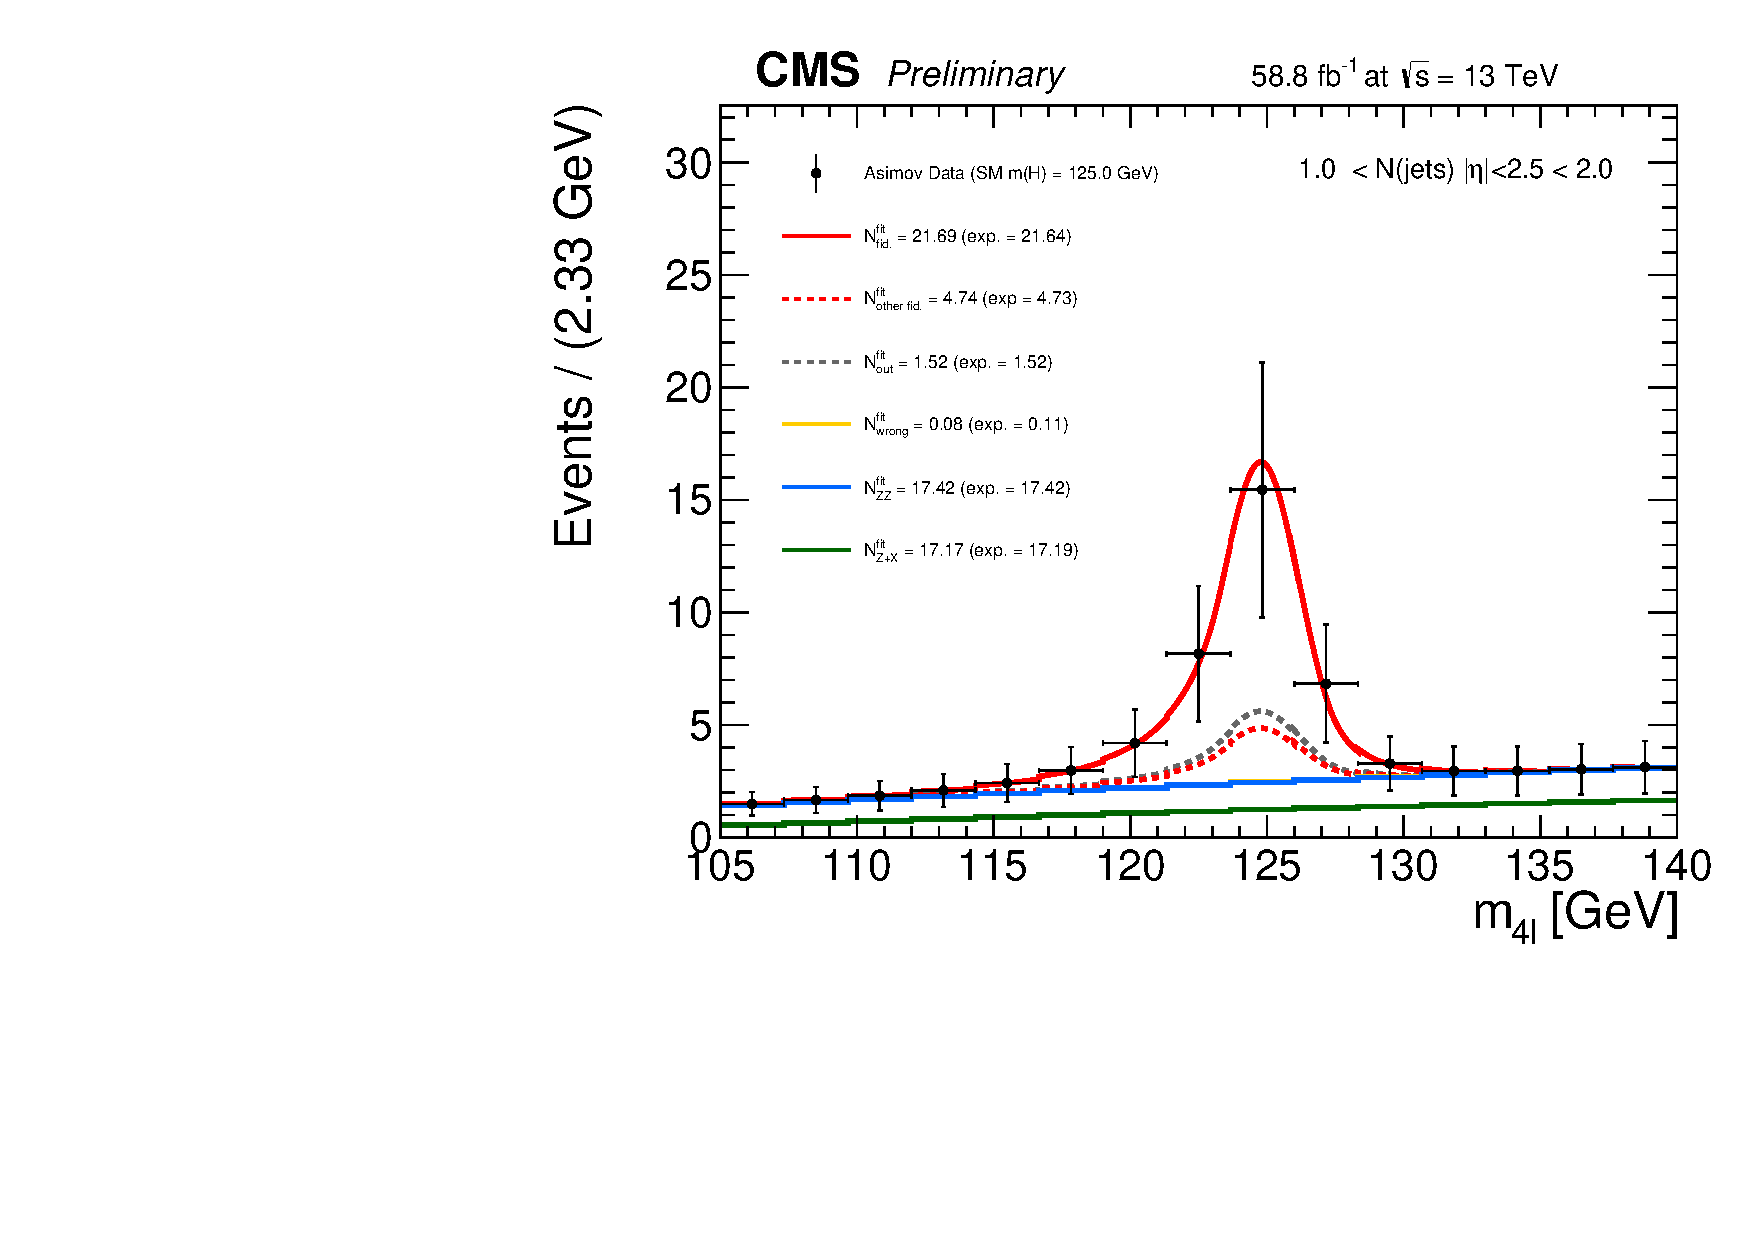
\includegraphics[width=0.32\linewidth]{Figures/results/fiducial/2018/asimovdata_SM_125_v2_unfoldwith_SM_125_v3_njets_pt30_eta2p5_4l_recobin1.pdf}
%	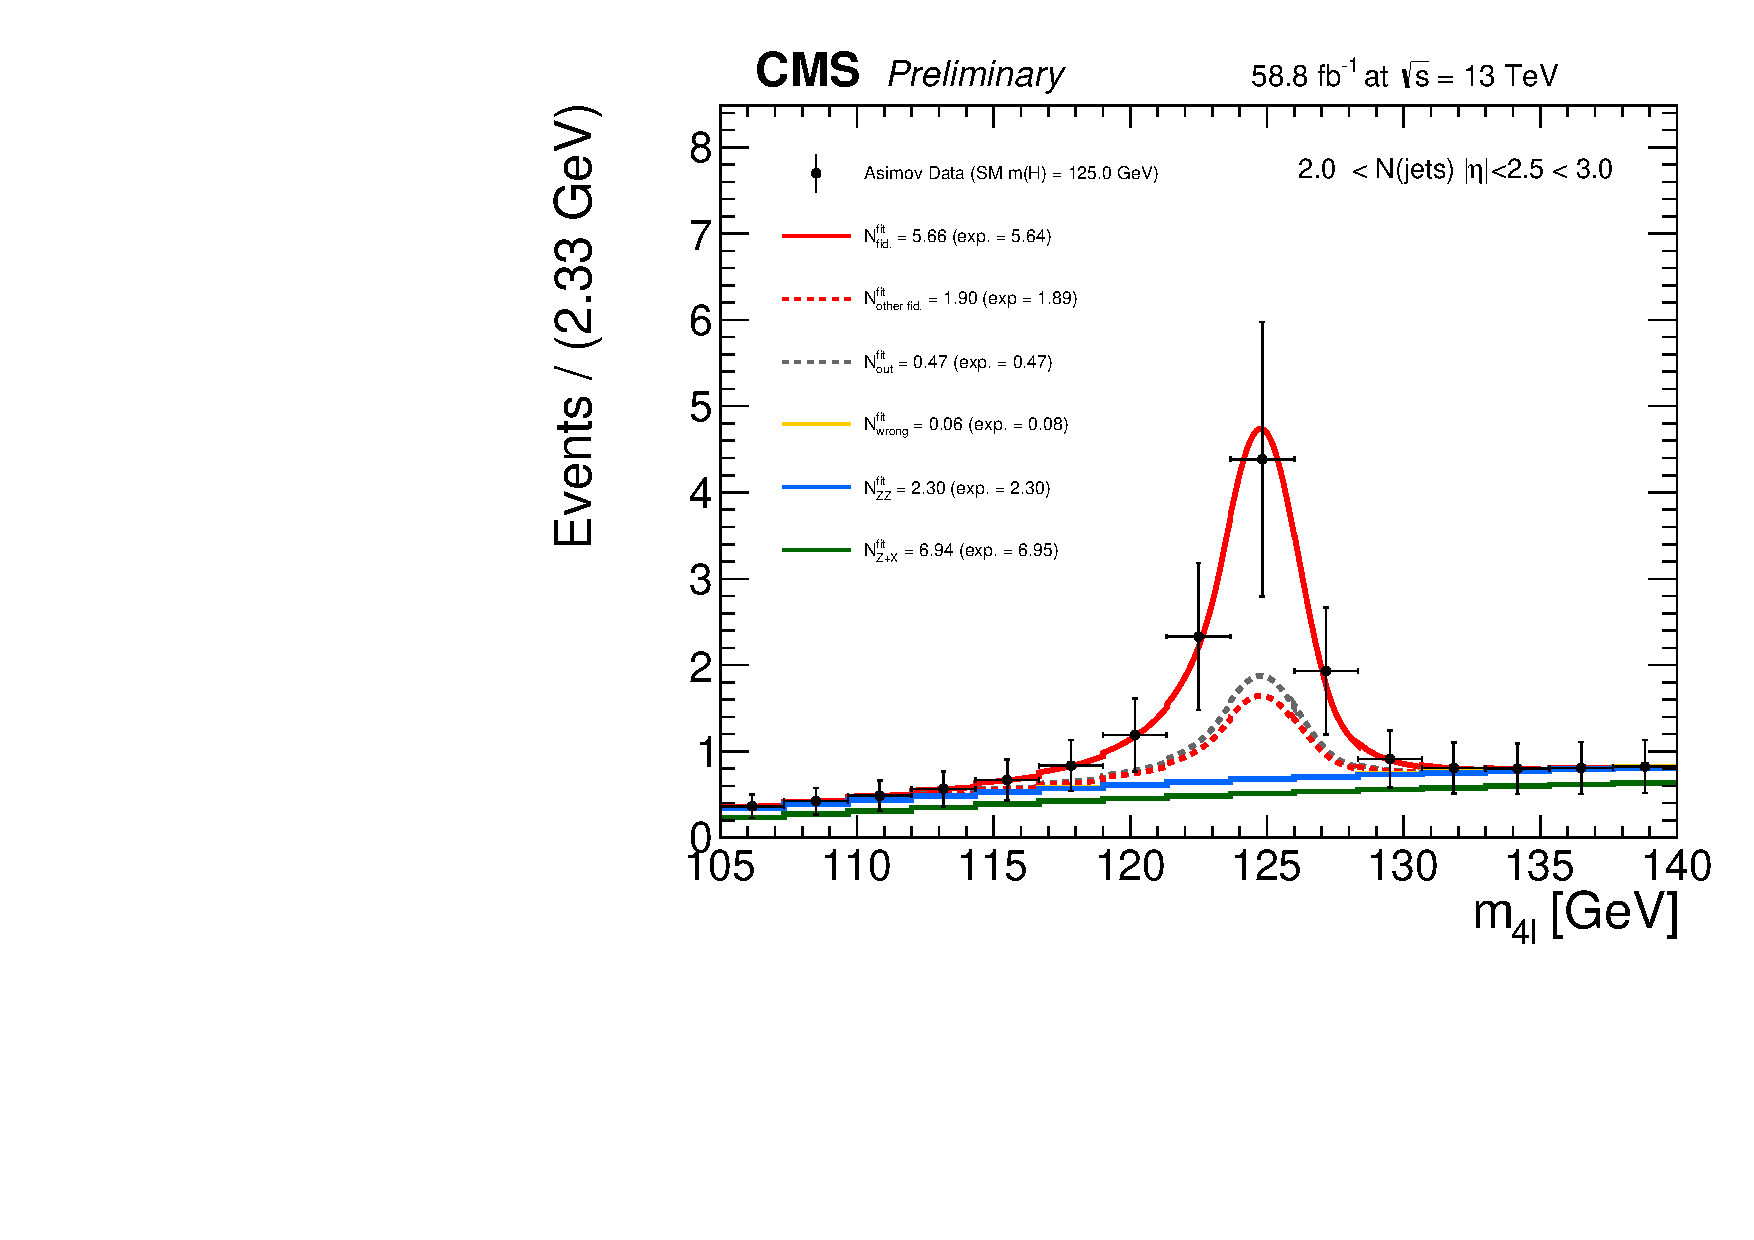
\includegraphics[width=0.32\linewidth]{Figures/results/fiducial/2018/asimovdata_SM_125_v2_unfoldwith_SM_125_v3_njets_pt30_eta2p5_4l_recobin2.pdf} \\
%	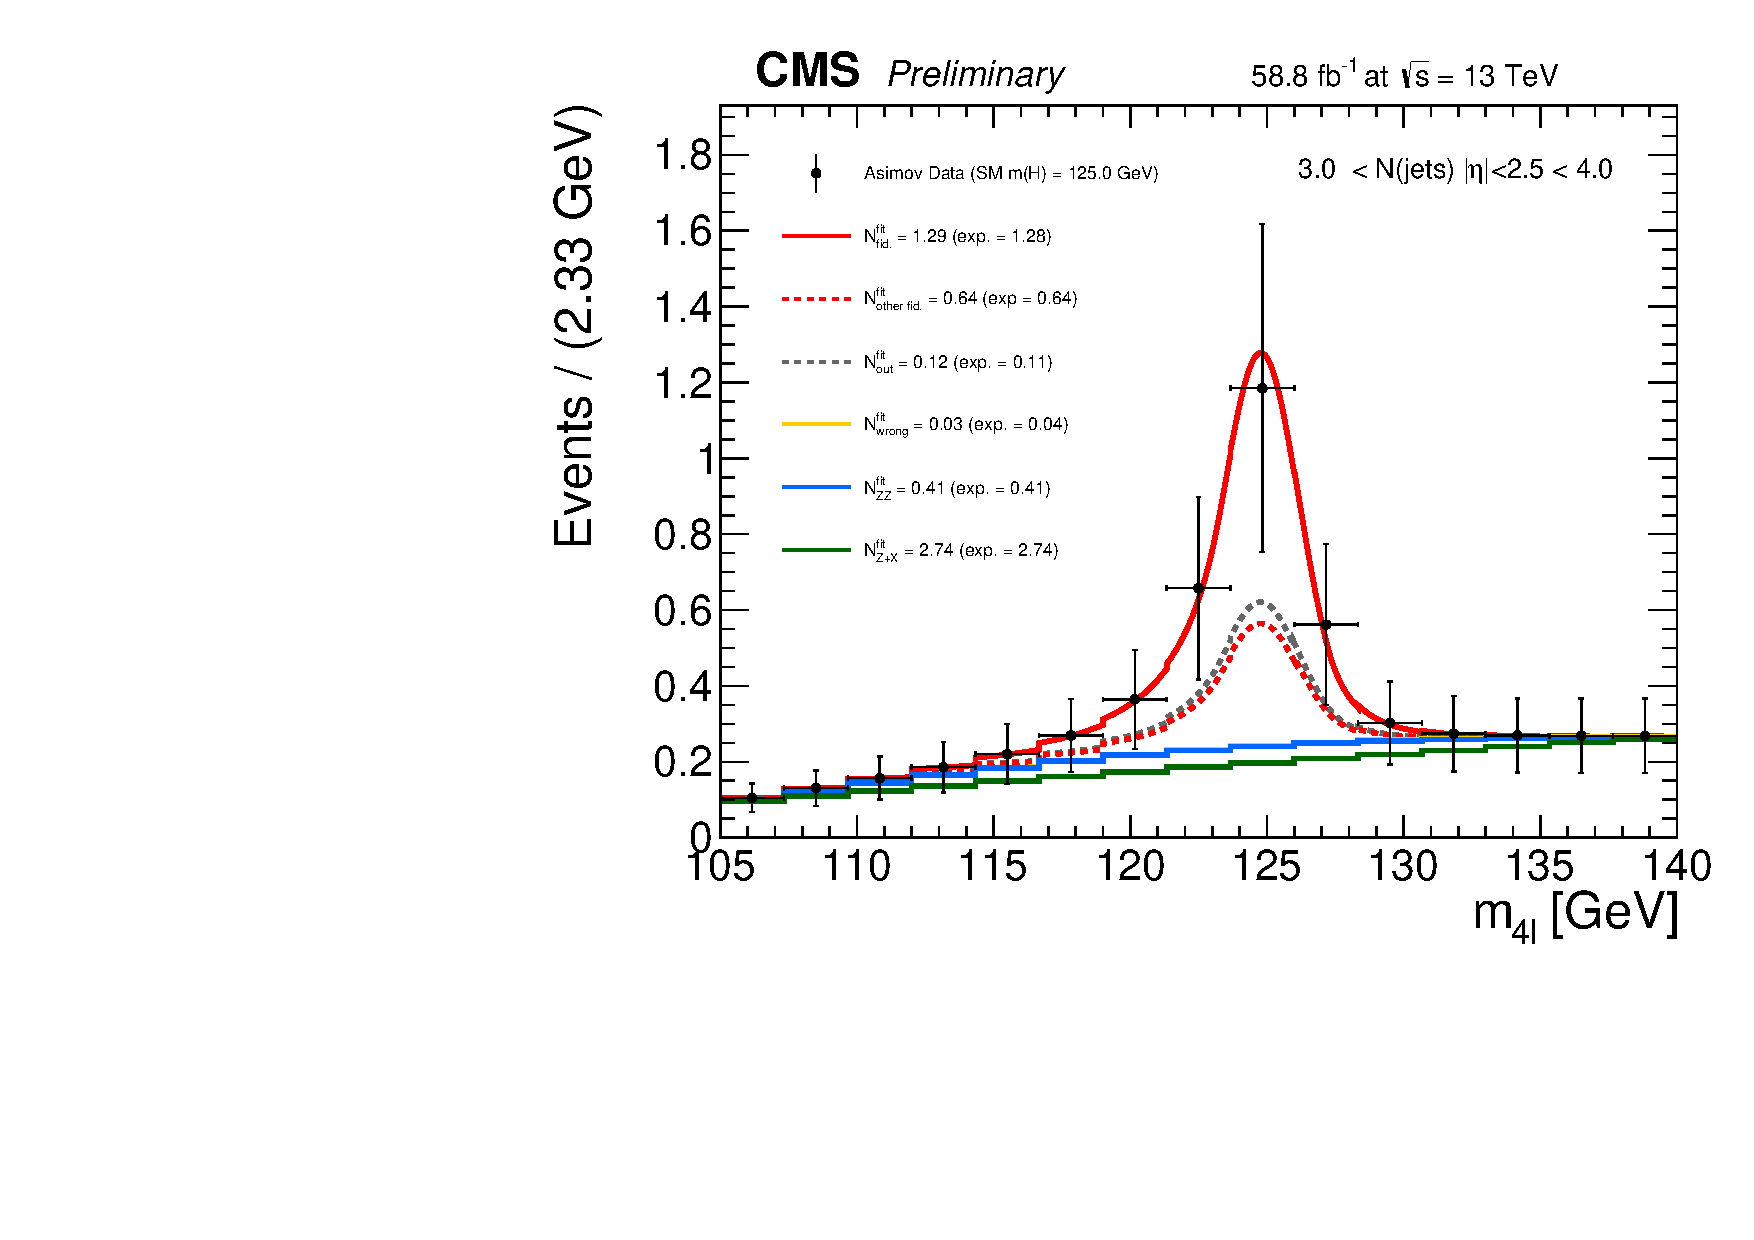
\includegraphics[width=0.32\linewidth]{Figures/results/fiducial/2018/asimovdata_SM_125_v2_unfoldwith_SM_125_v3_njets_pt30_eta2p5_4l_recobin3.pdf}
%	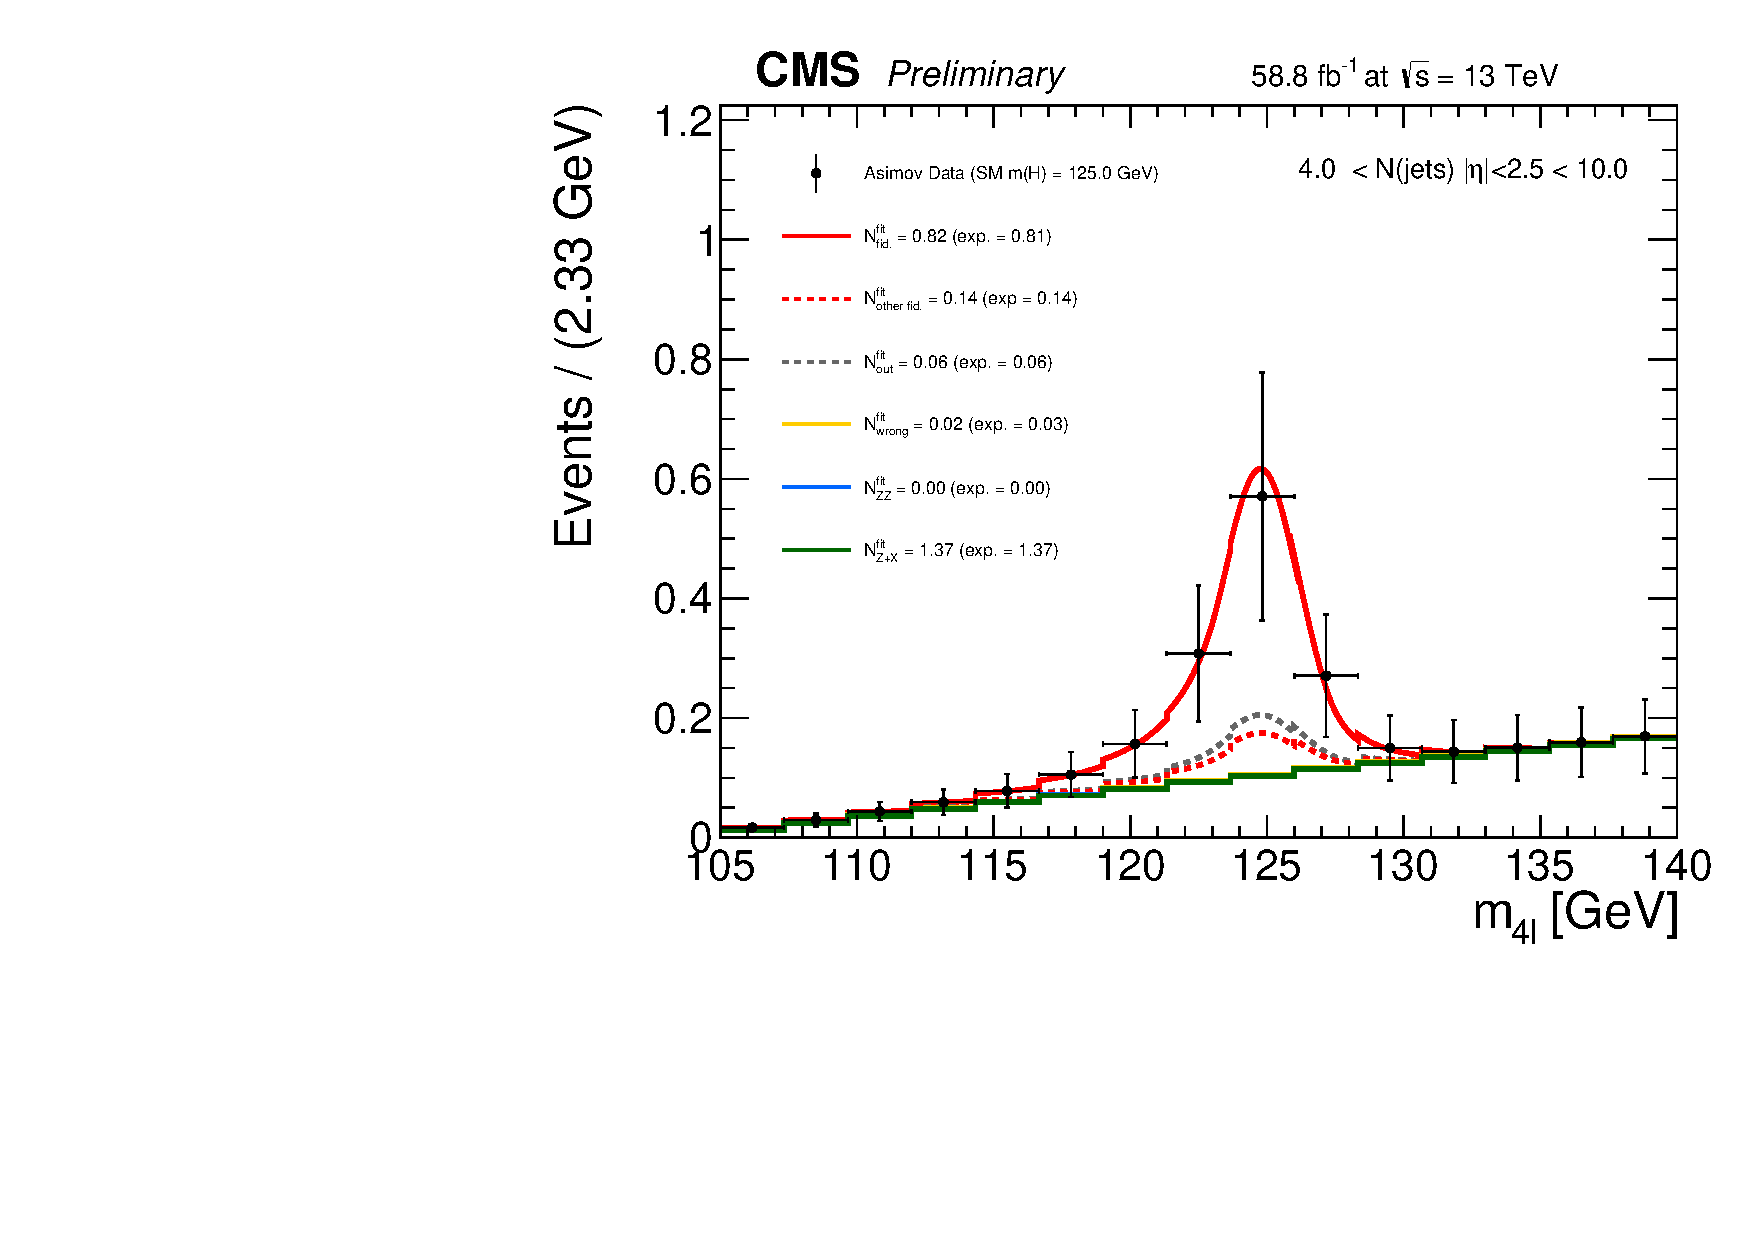
\includegraphics[width=0.32\linewidth]{Figures/results/fiducial/2018/asimovdata_SM_125_v2_unfoldwith_SM_125_v3_njets_pt30_eta2p5_4l_recobin4.pdf}
%	\caption{Result of simultaneous fit for the differential fiducial cross subsection measurement for N(jets) 
%		in each differential bin. The combined 4$\ell$ final state is shown. The results are shown for 2018 only. \label{fig:differentialfitNjets}}
%\end{figure}
%
%\begin{figure}[!h]
%	\centering
%	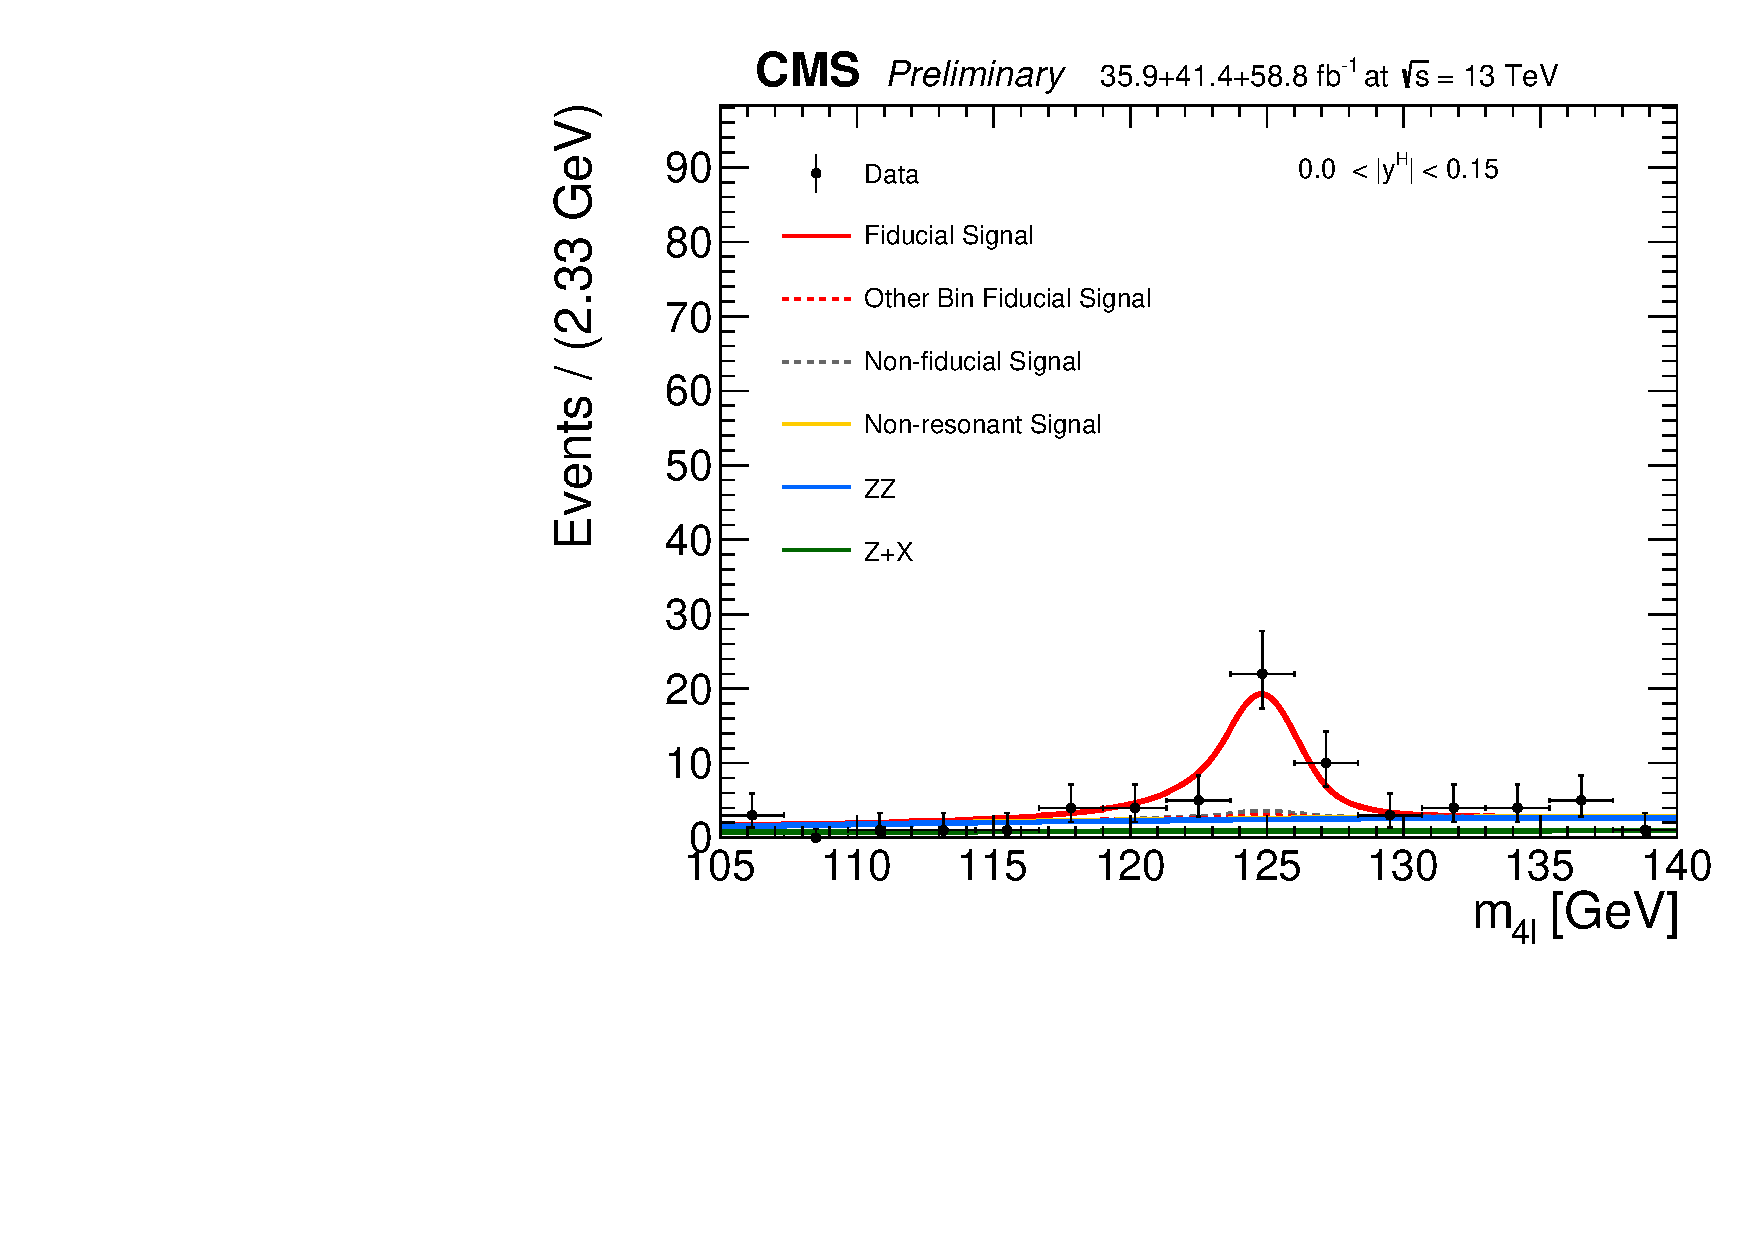
\includegraphics[width=0.32\linewidth]{Figures/results/fiducial/comb/unblind_Feb25/data_unfoldwith_SM_125_v3_rapidity4l_4l_recobin0.pdf}
%	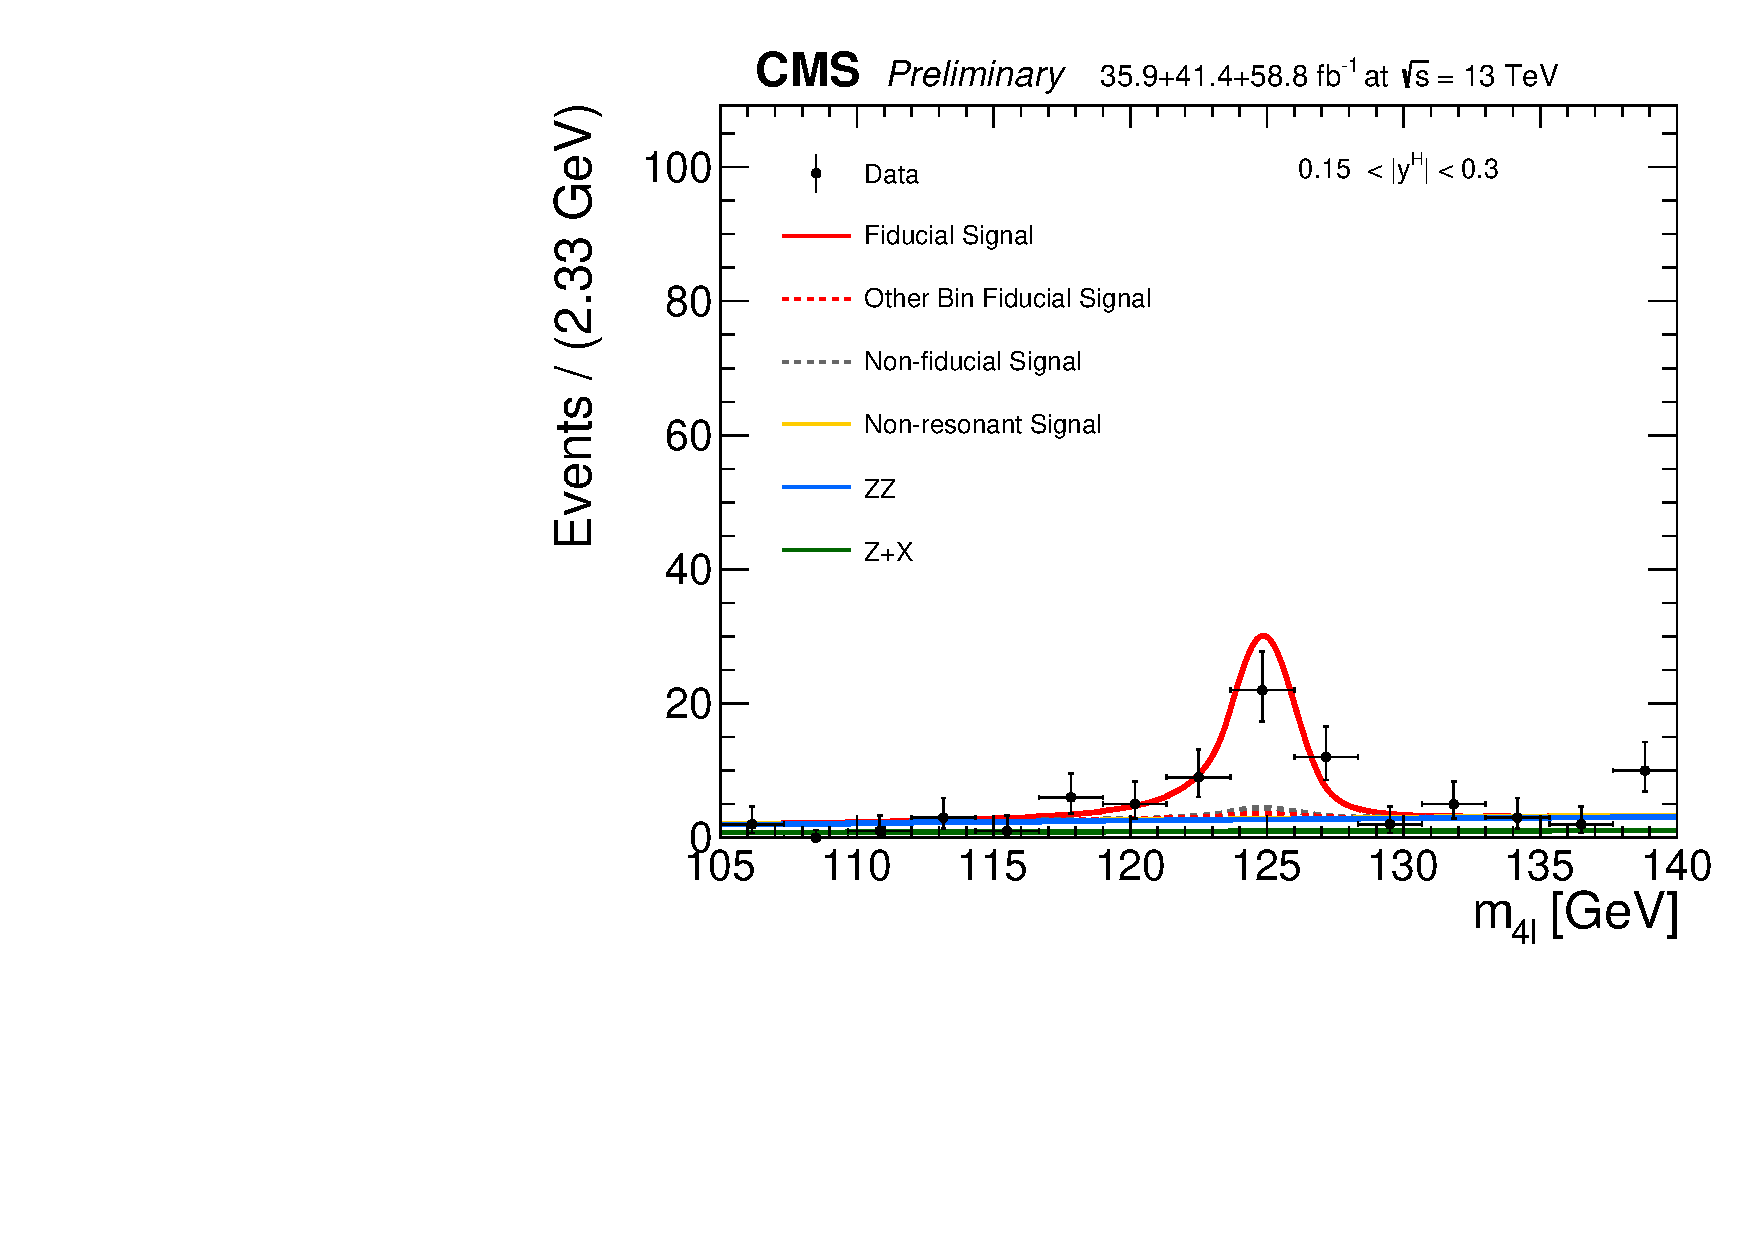
\includegraphics[width=0.32\linewidth]{Figures/results/fiducial/comb/unblind_Feb25/data_unfoldwith_SM_125_v3_rapidity4l_4l_recobin1.pdf}
%	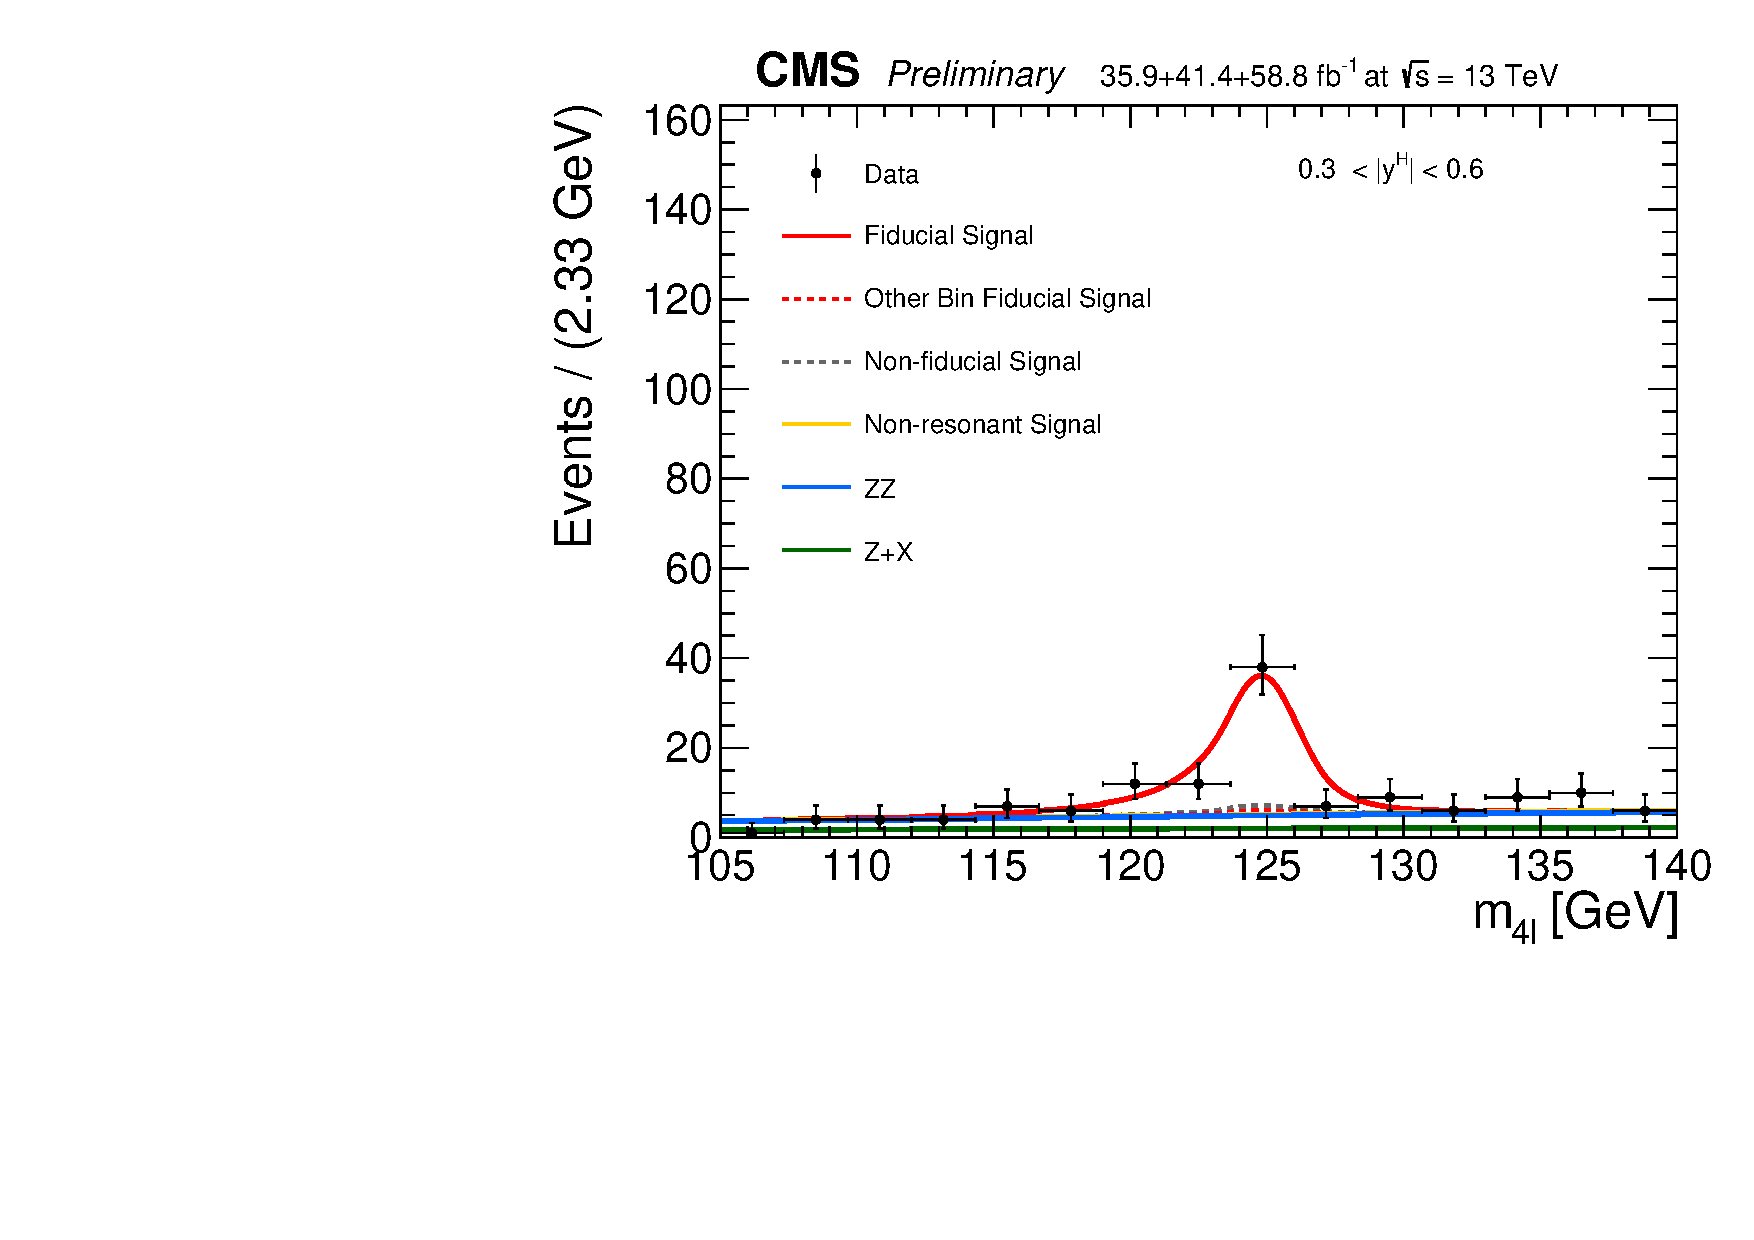
\includegraphics[width=0.32\linewidth]{Figures/results/fiducial/comb/unblind_Feb25/data_unfoldwith_SM_125_v3_rapidity4l_4l_recobin2.pdf} \\
%	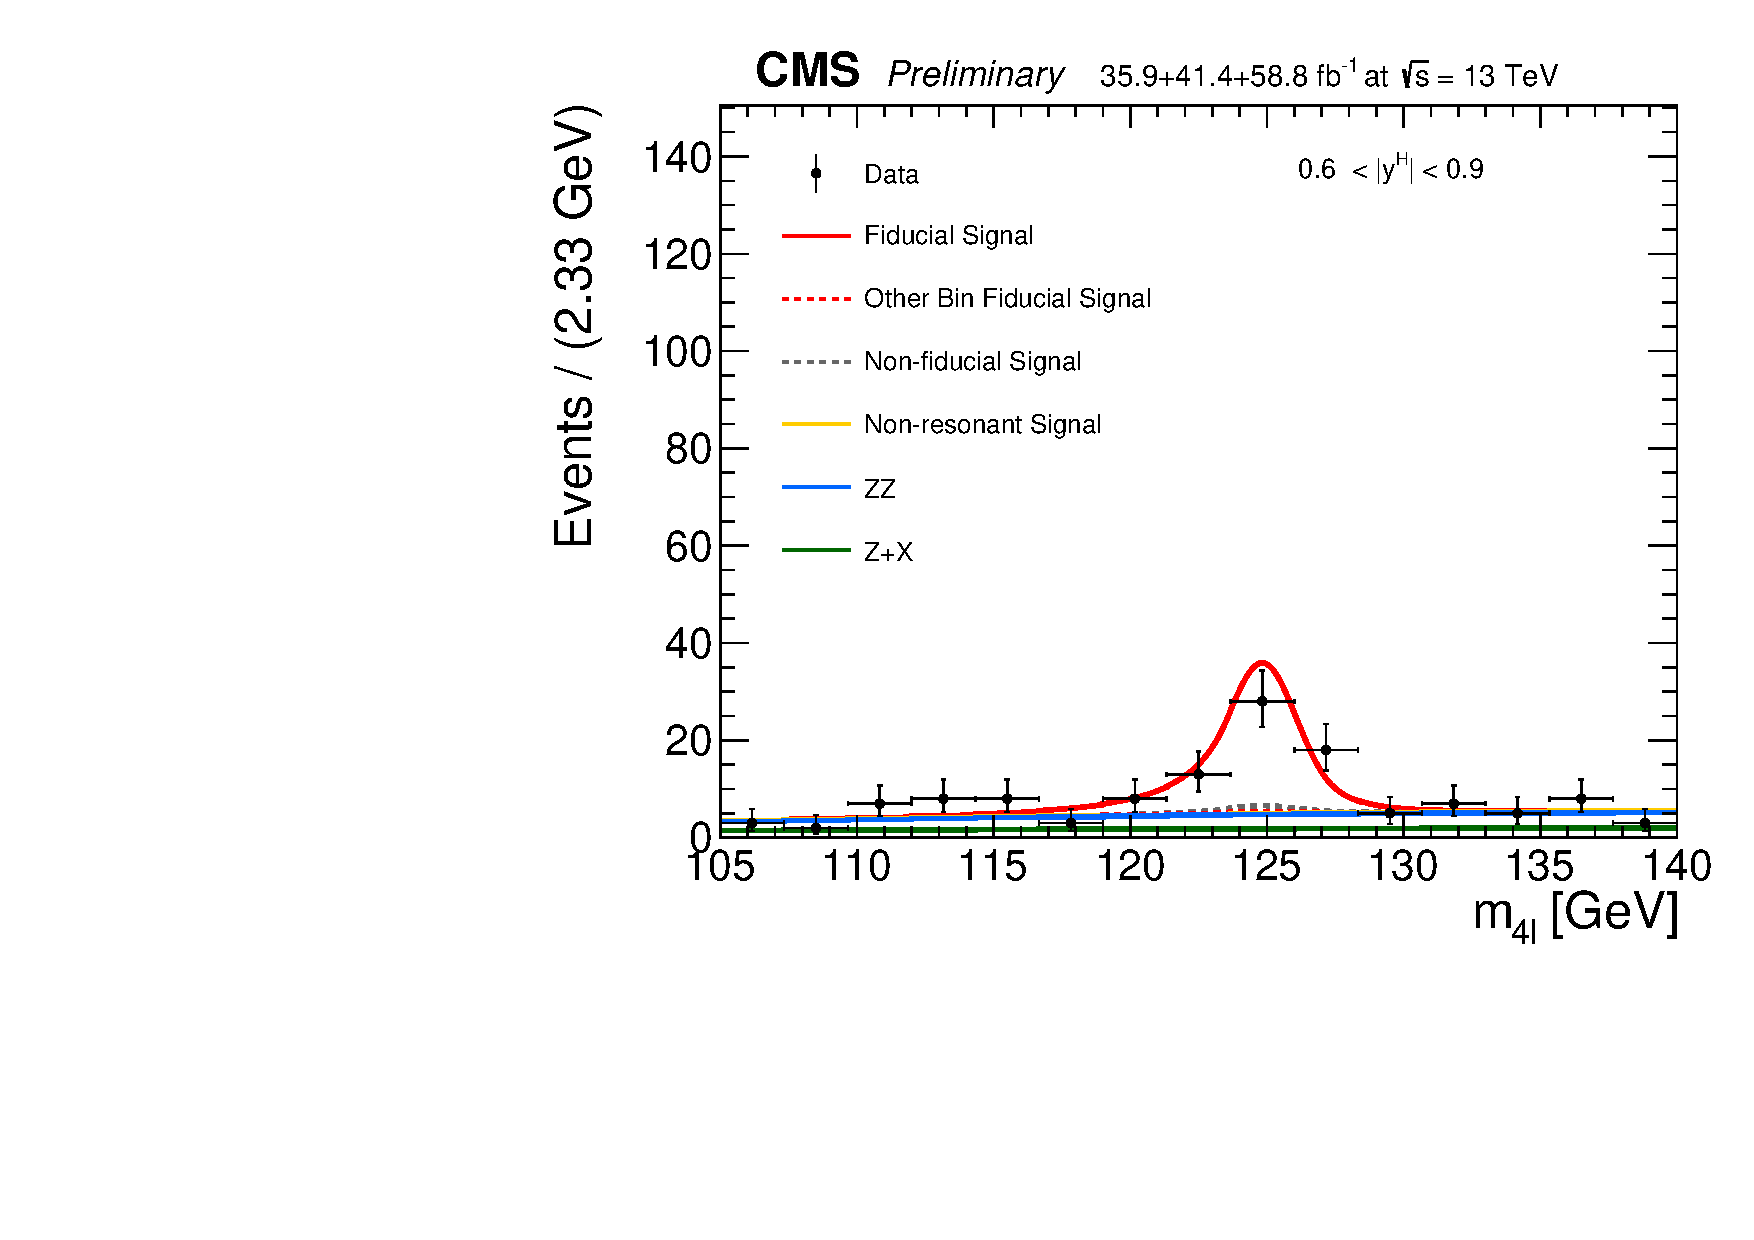
\includegraphics[width=0.32\linewidth]{Figures/results/fiducial/comb/unblind_Feb25/data_unfoldwith_SM_125_v3_rapidity4l_4l_recobin3.pdf}
%	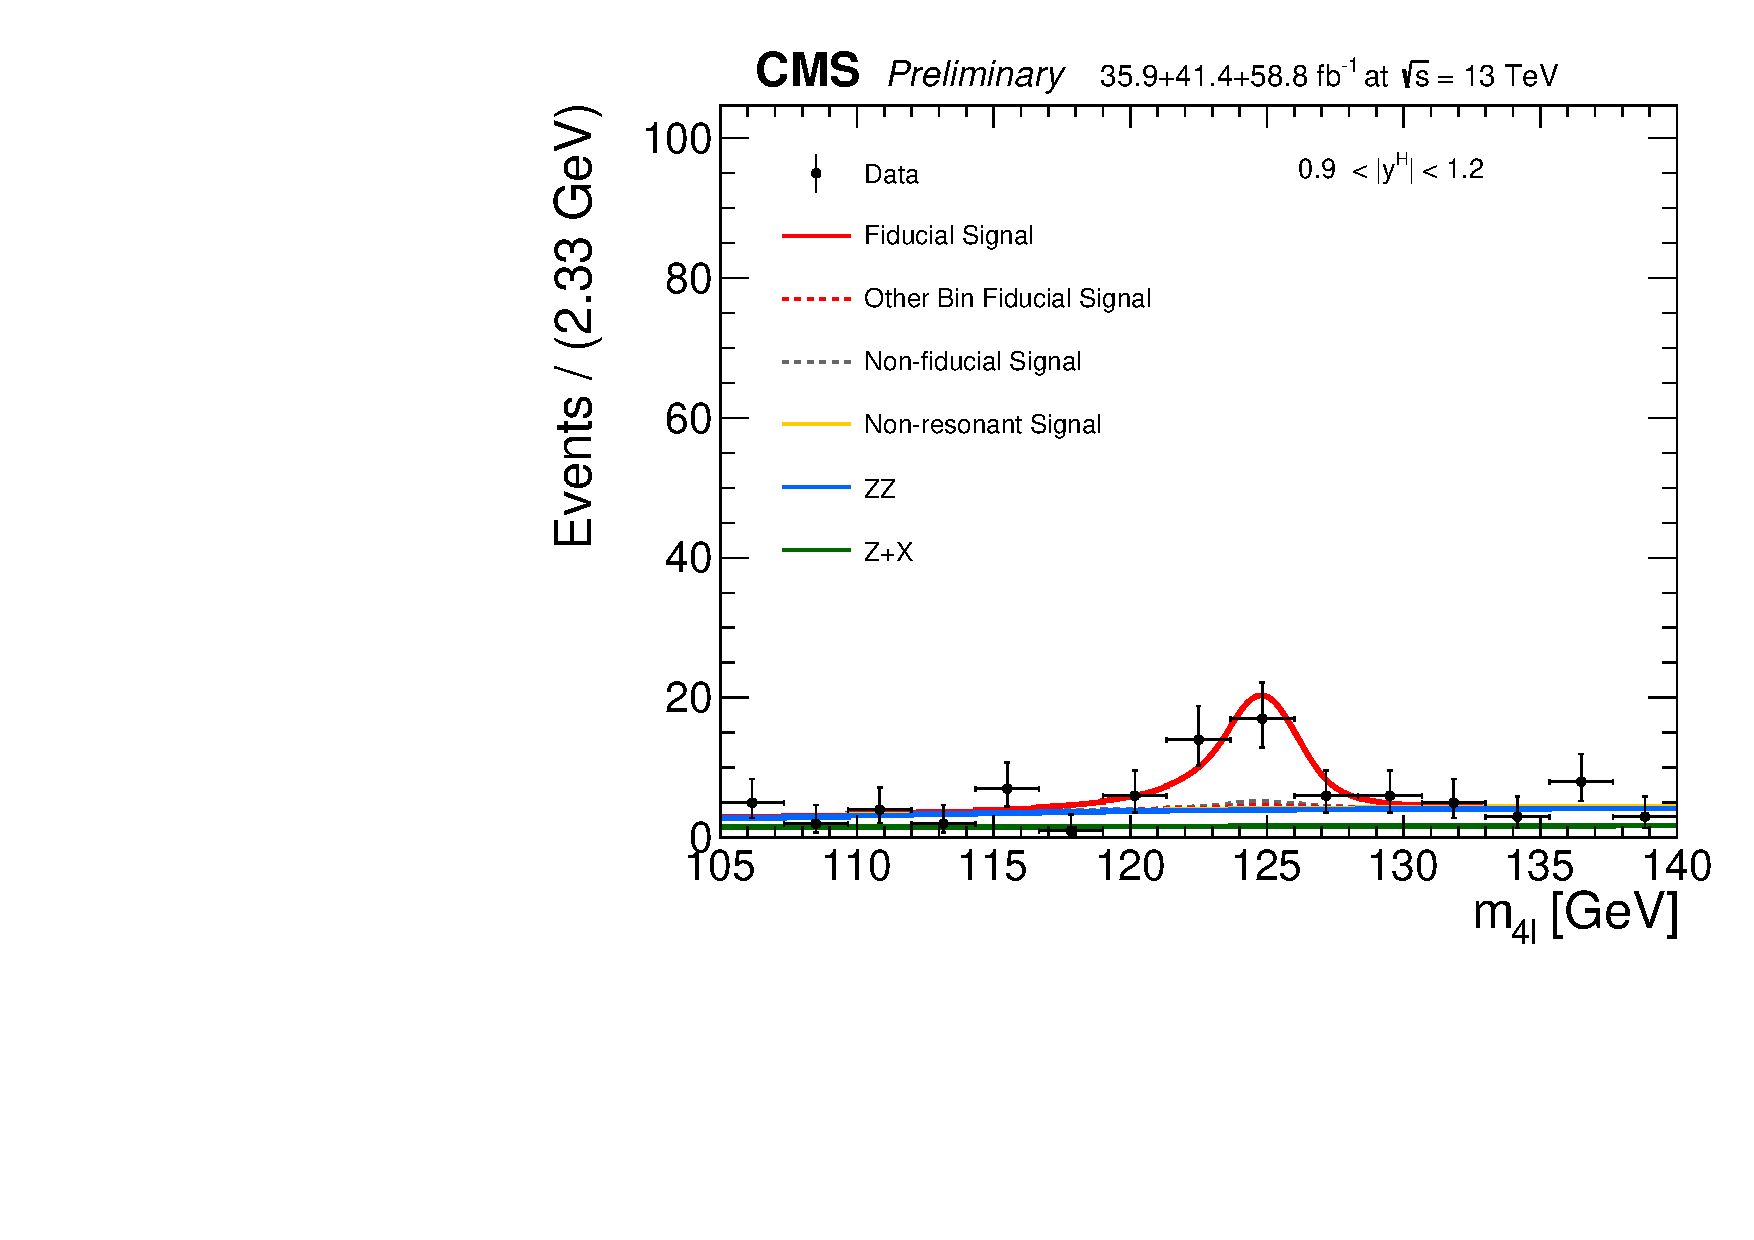
\includegraphics[width=0.32\linewidth]{Figures/results/fiducial/comb/unblind_Feb25/data_unfoldwith_SM_125_v3_rapidity4l_4l_recobin4.pdf}
%	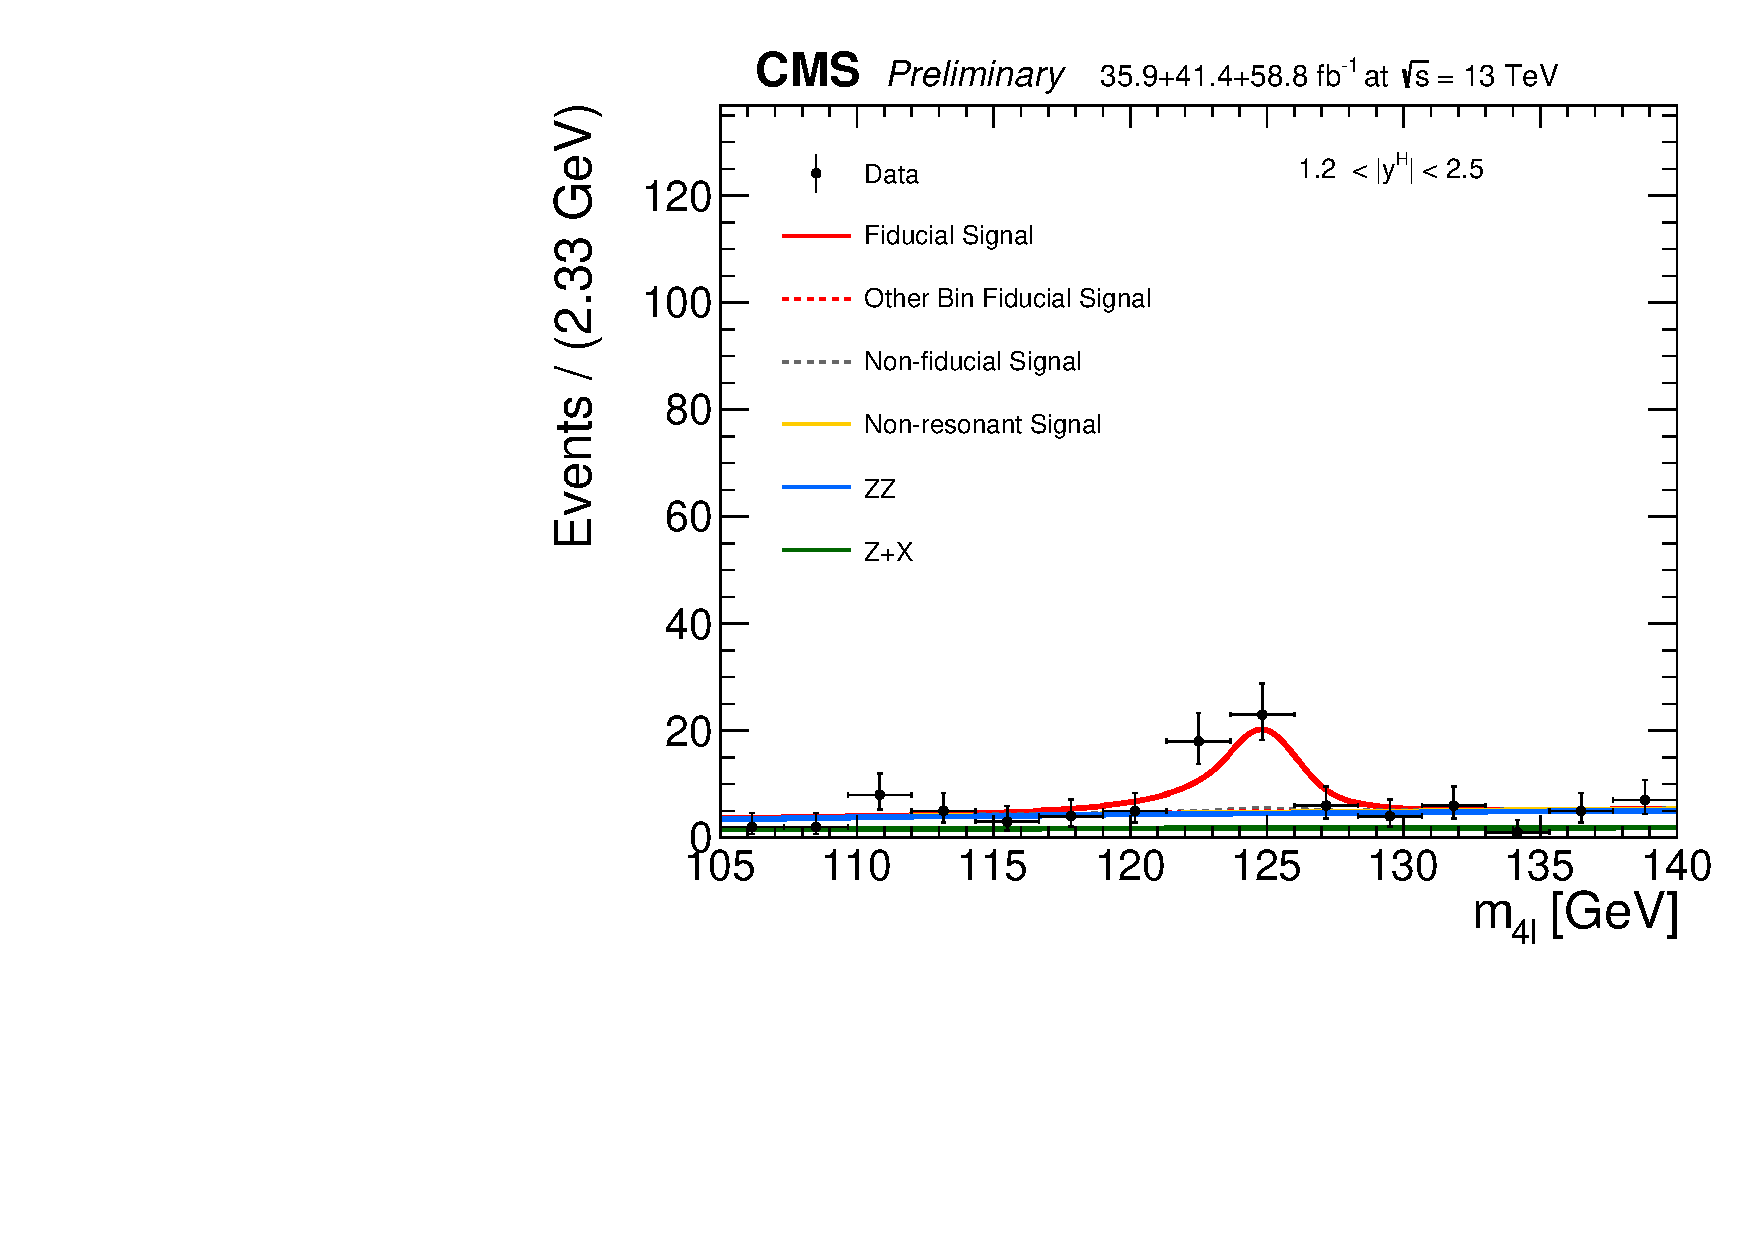
\includegraphics[width=0.32\linewidth]{Figures/results/fiducial/comb/unblind_Feb25/data_unfoldwith_SM_125_v3_rapidity4l_4l_recobin5.pdf}
%	\caption{Result of simultaneous fit for the differential fiducial cross subsection measurement for $y(H)$
%		in each differential bin. The combined 4$\ell$ final state is shown. The results are shown for 2018 only. \label{fig:differentialfitNjets}}
%\end{figure}
%
%
%The expected differential cross subsection results can be seen in Fig.~\ref{fig:fiducialresult}. 
%
%%\begin{figure}[!h]
%%	\centering
%%	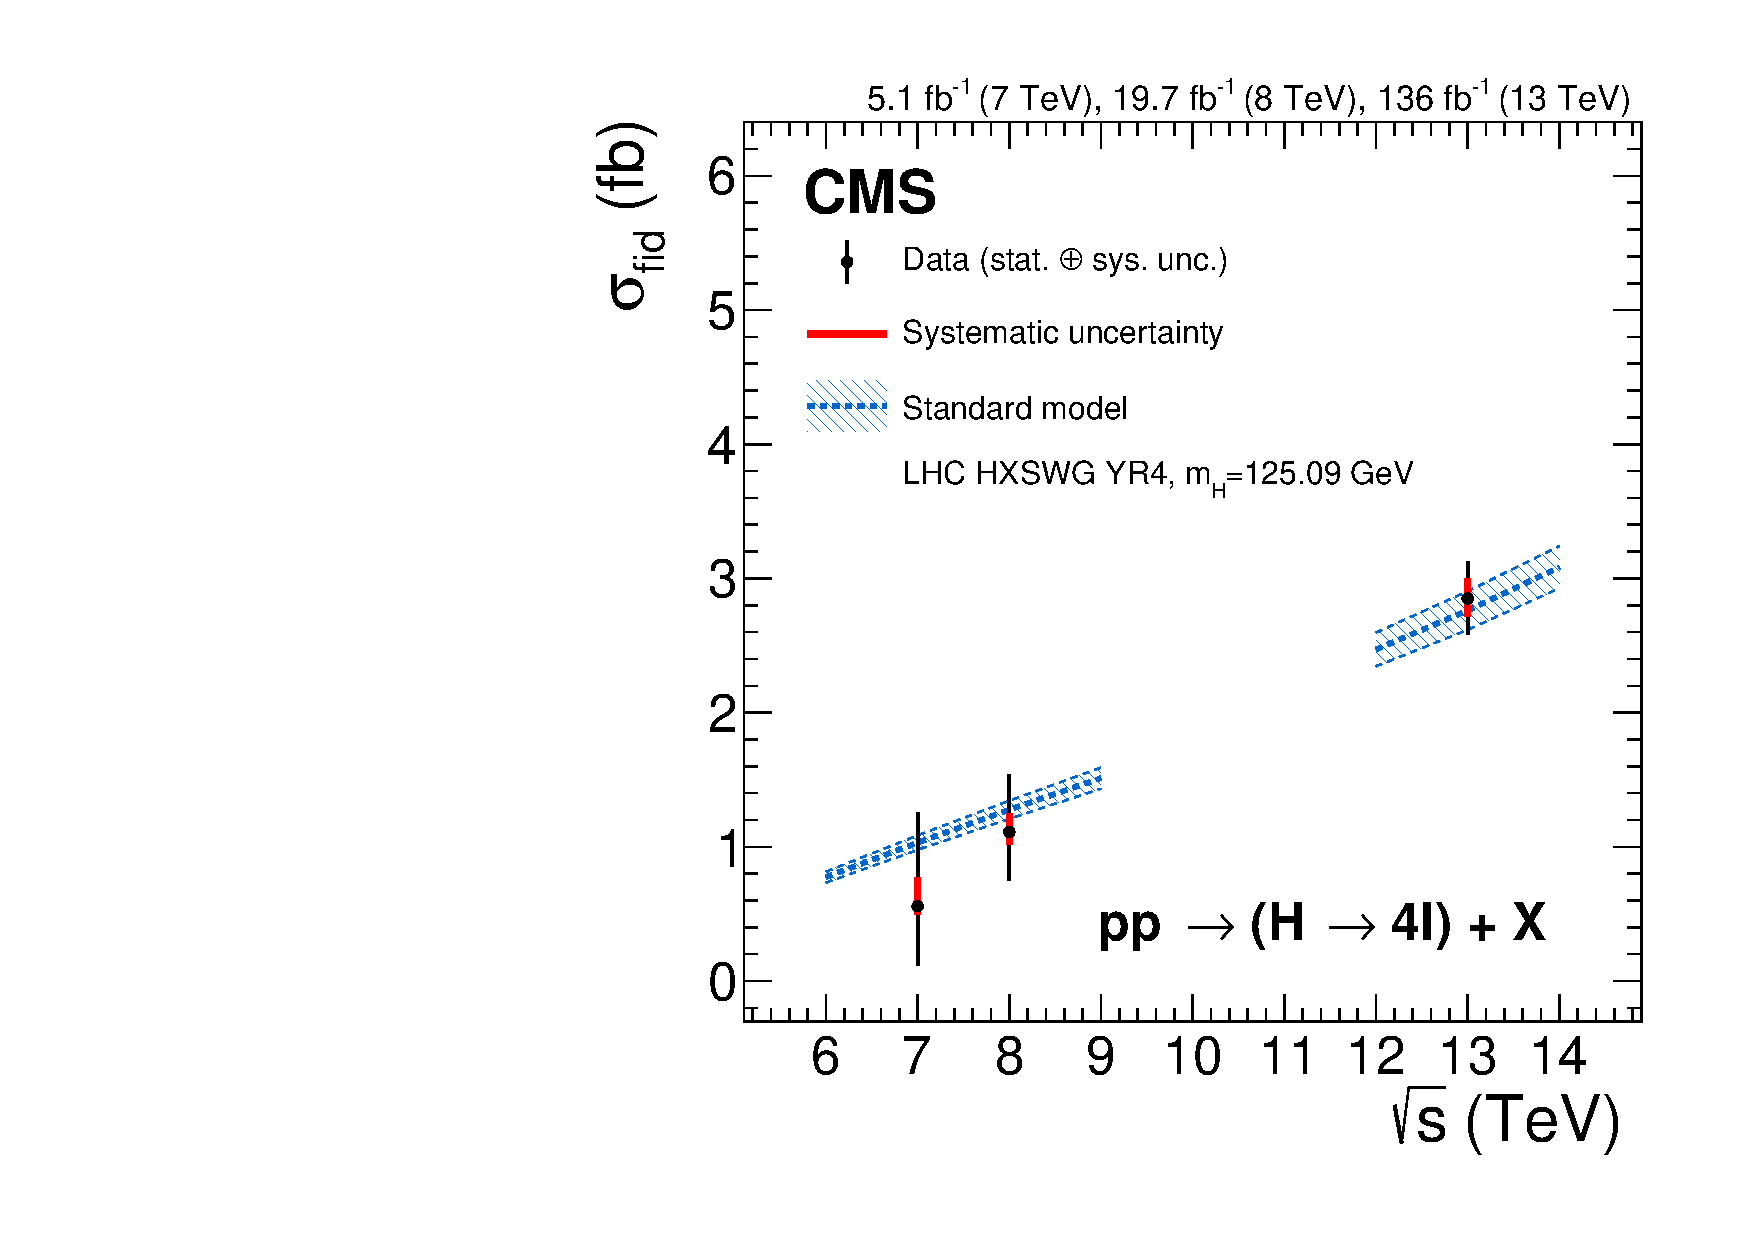
\includegraphics[width=0.45\linewidth]{Figures/results/fiducial/comb/unblind_Feb25/xs_vs_sqrts.pdf}
%    % this one is 2016 scaled, to be fixed
%%	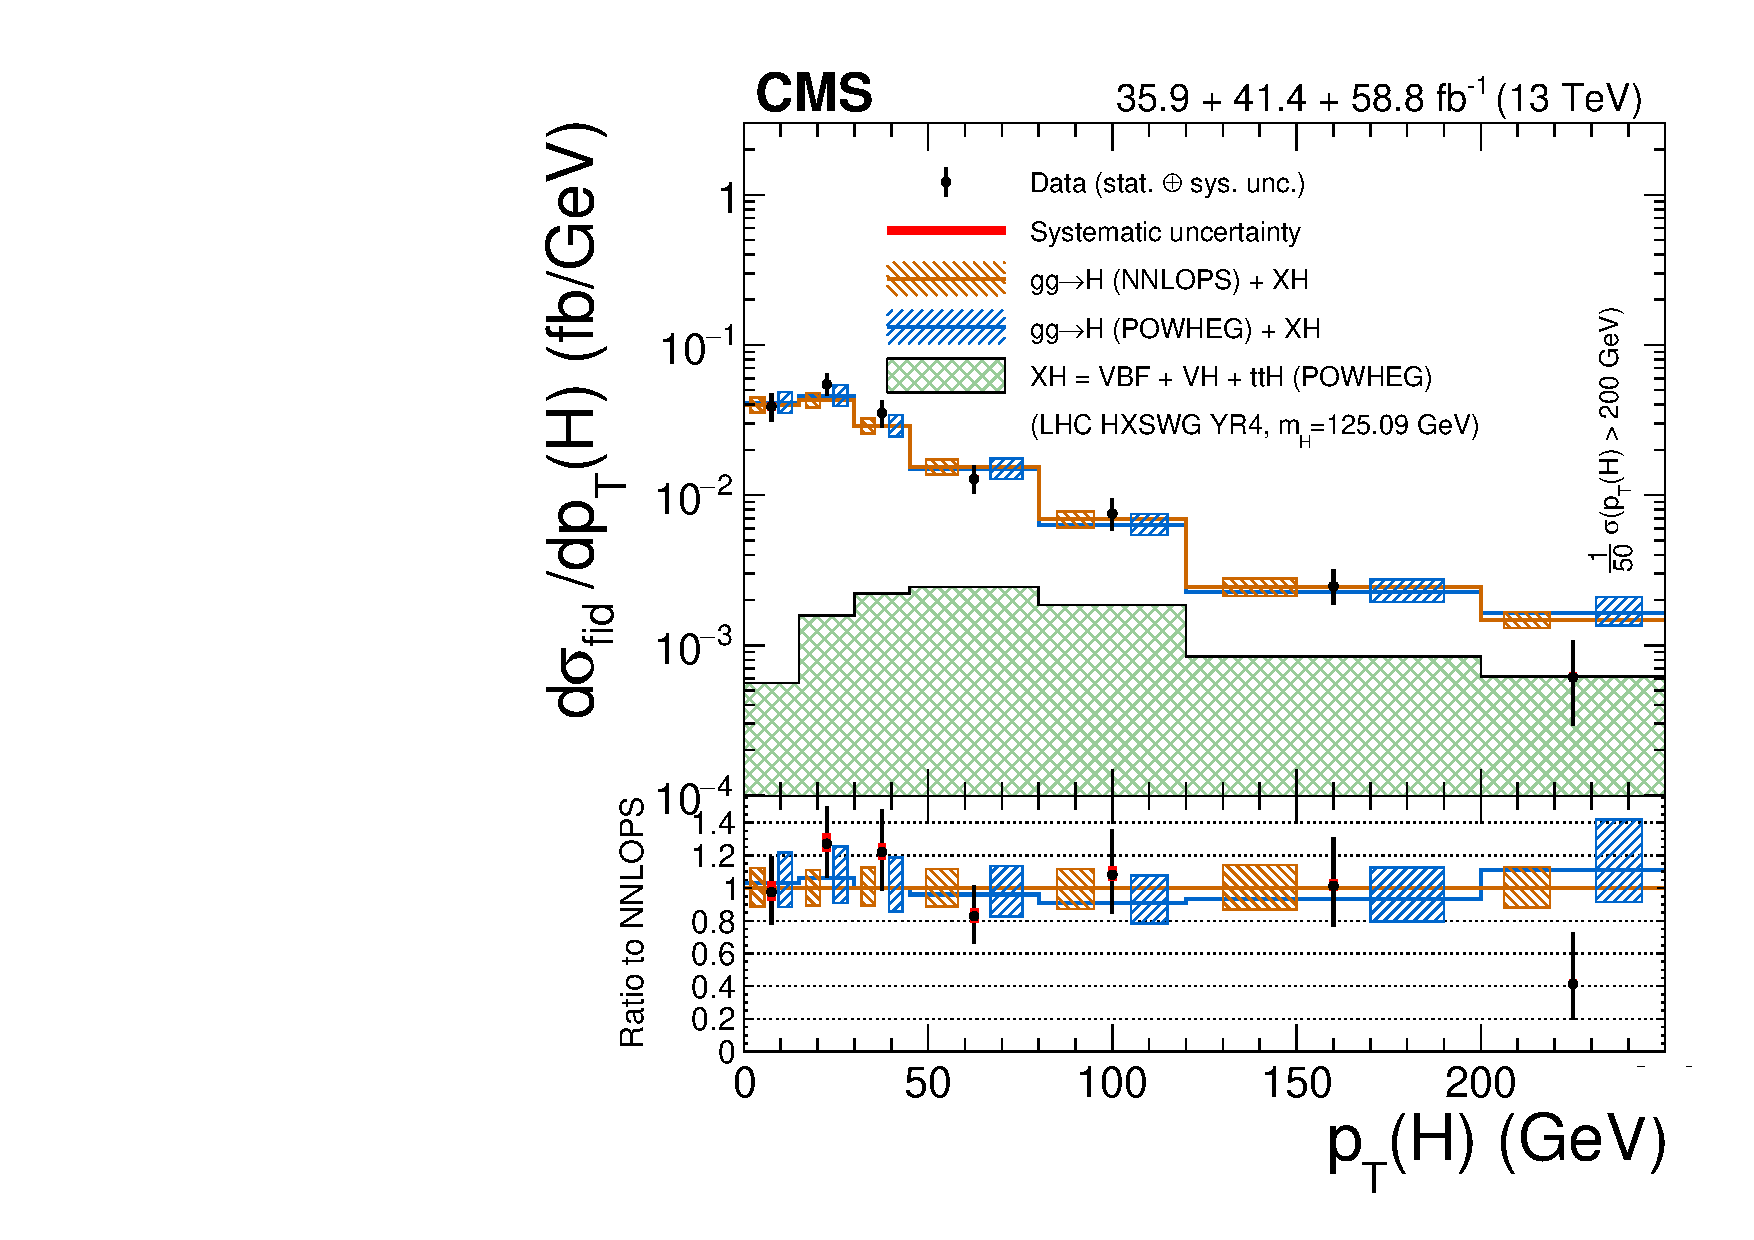
\includegraphics[width=0.45\linewidth]{Figures/results/fiducial/comb/unblind_Feb25/pT4l_unfoldwith_SM_125_logscale.pdf} \\
%%	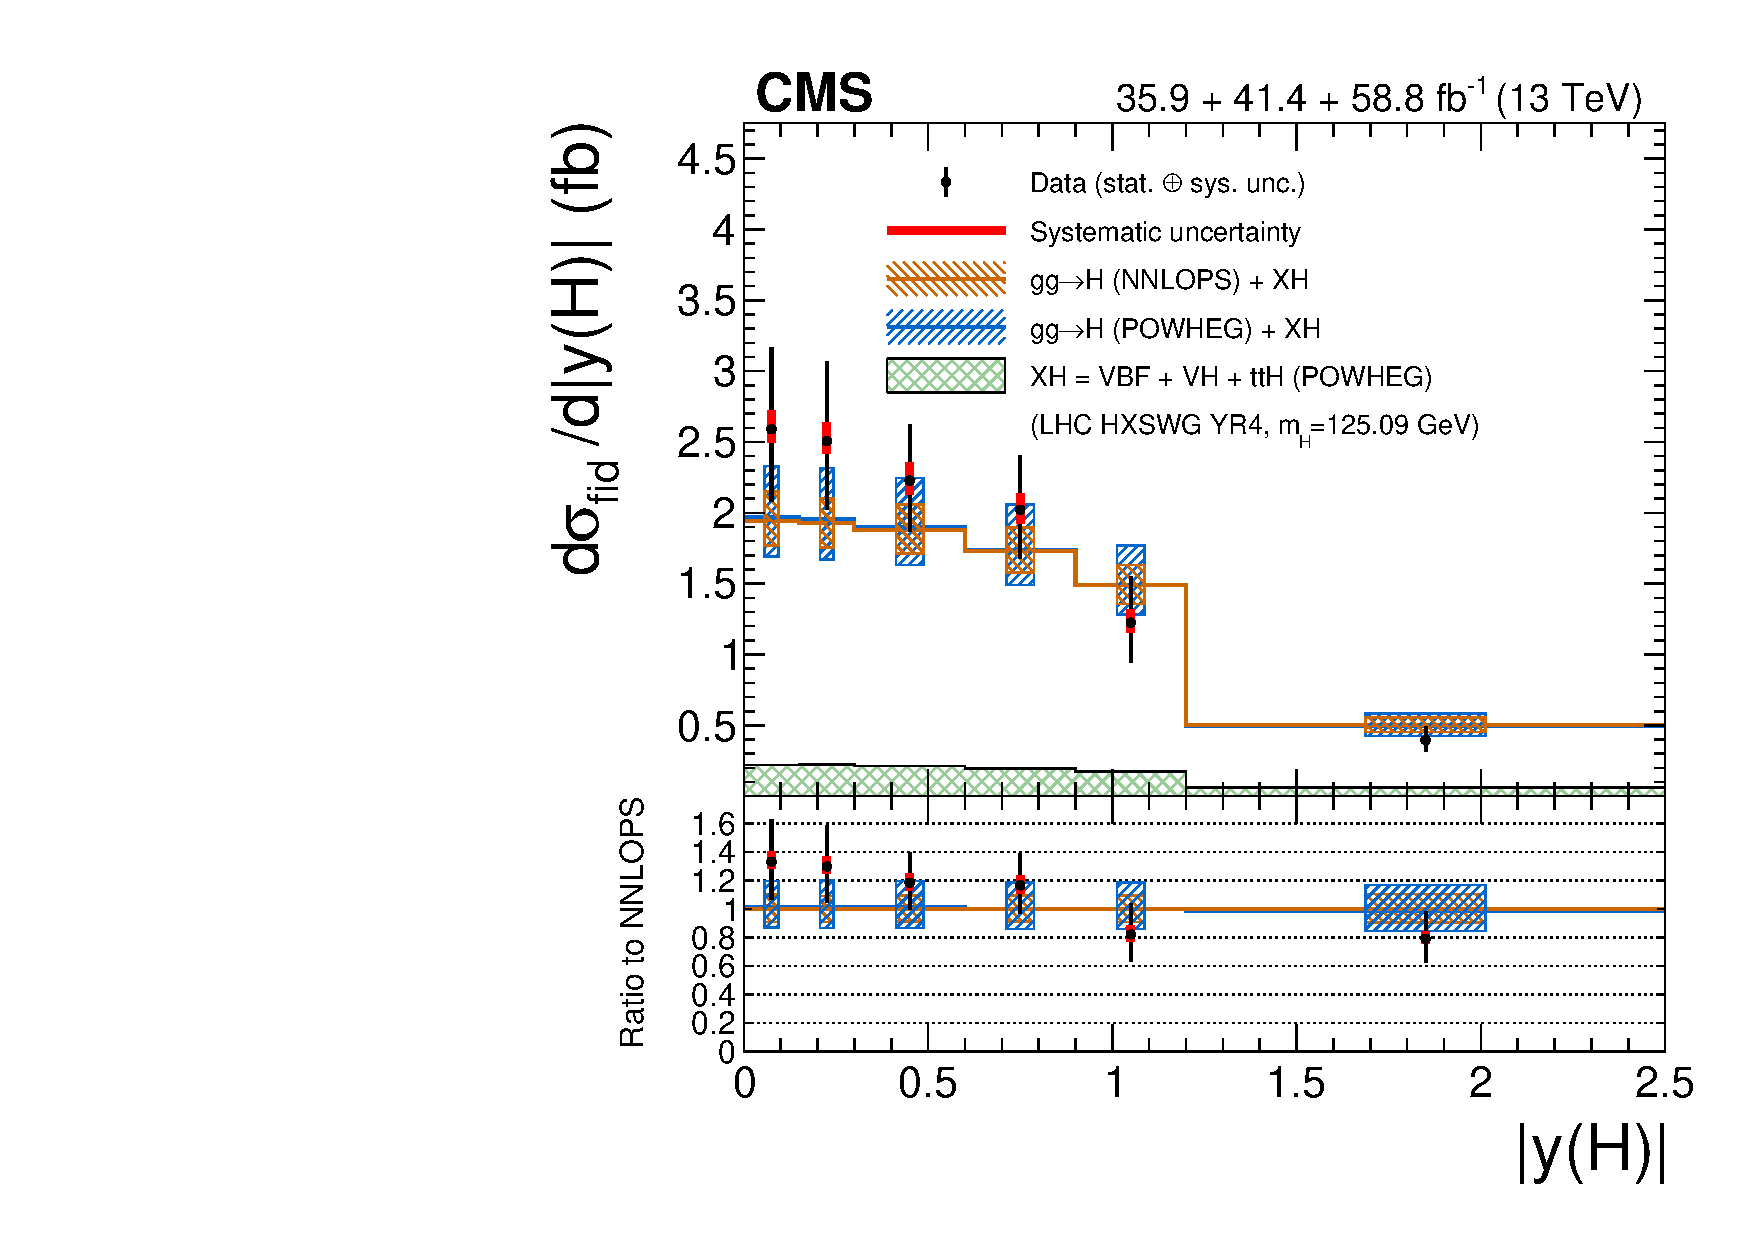
\includegraphics[width=0.45\linewidth]{Figures/results/fiducial/comb/unblind_Feb25/rapidity4l_unfoldwith_SM_125.pdf}
%%	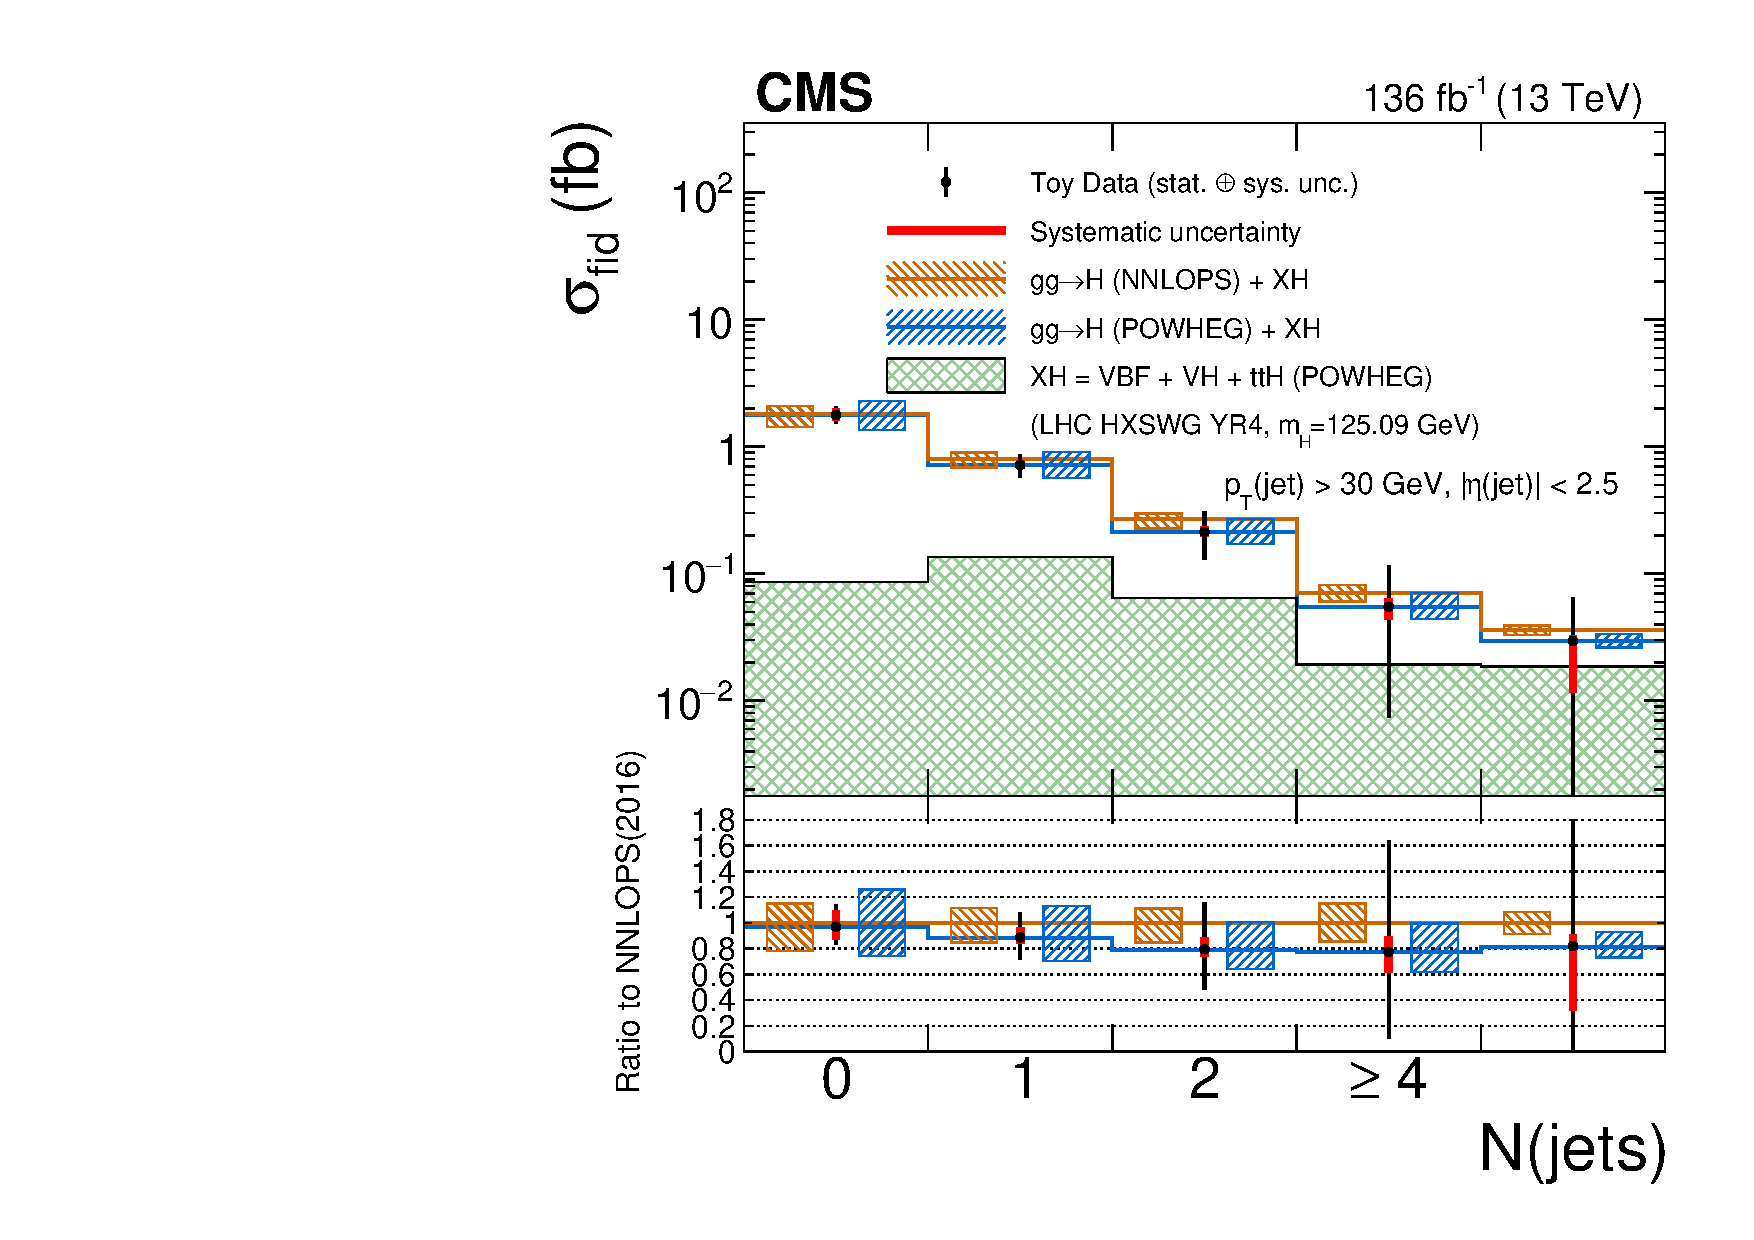
\includegraphics[width=0.45\linewidth]{Figures/results/fiducial/comb/scaled_2018/njets_pt30_eta2p5_unfoldwith_SM_125_logscale_asimov.pdf}
%%	\caption{Result of the integrated fiducial cross subsection and the differential cross subsection measurements for $\pt({\rm H})$, $y({\rm H}$, and N(jets). {\color{red} Lepton scale factors are uncorrelated across years. N(jets) still asimov.} \label{fig:differentialresult}}
%%\end{figure}
%
%\begin{figure}[!htb]
%        \centering
%        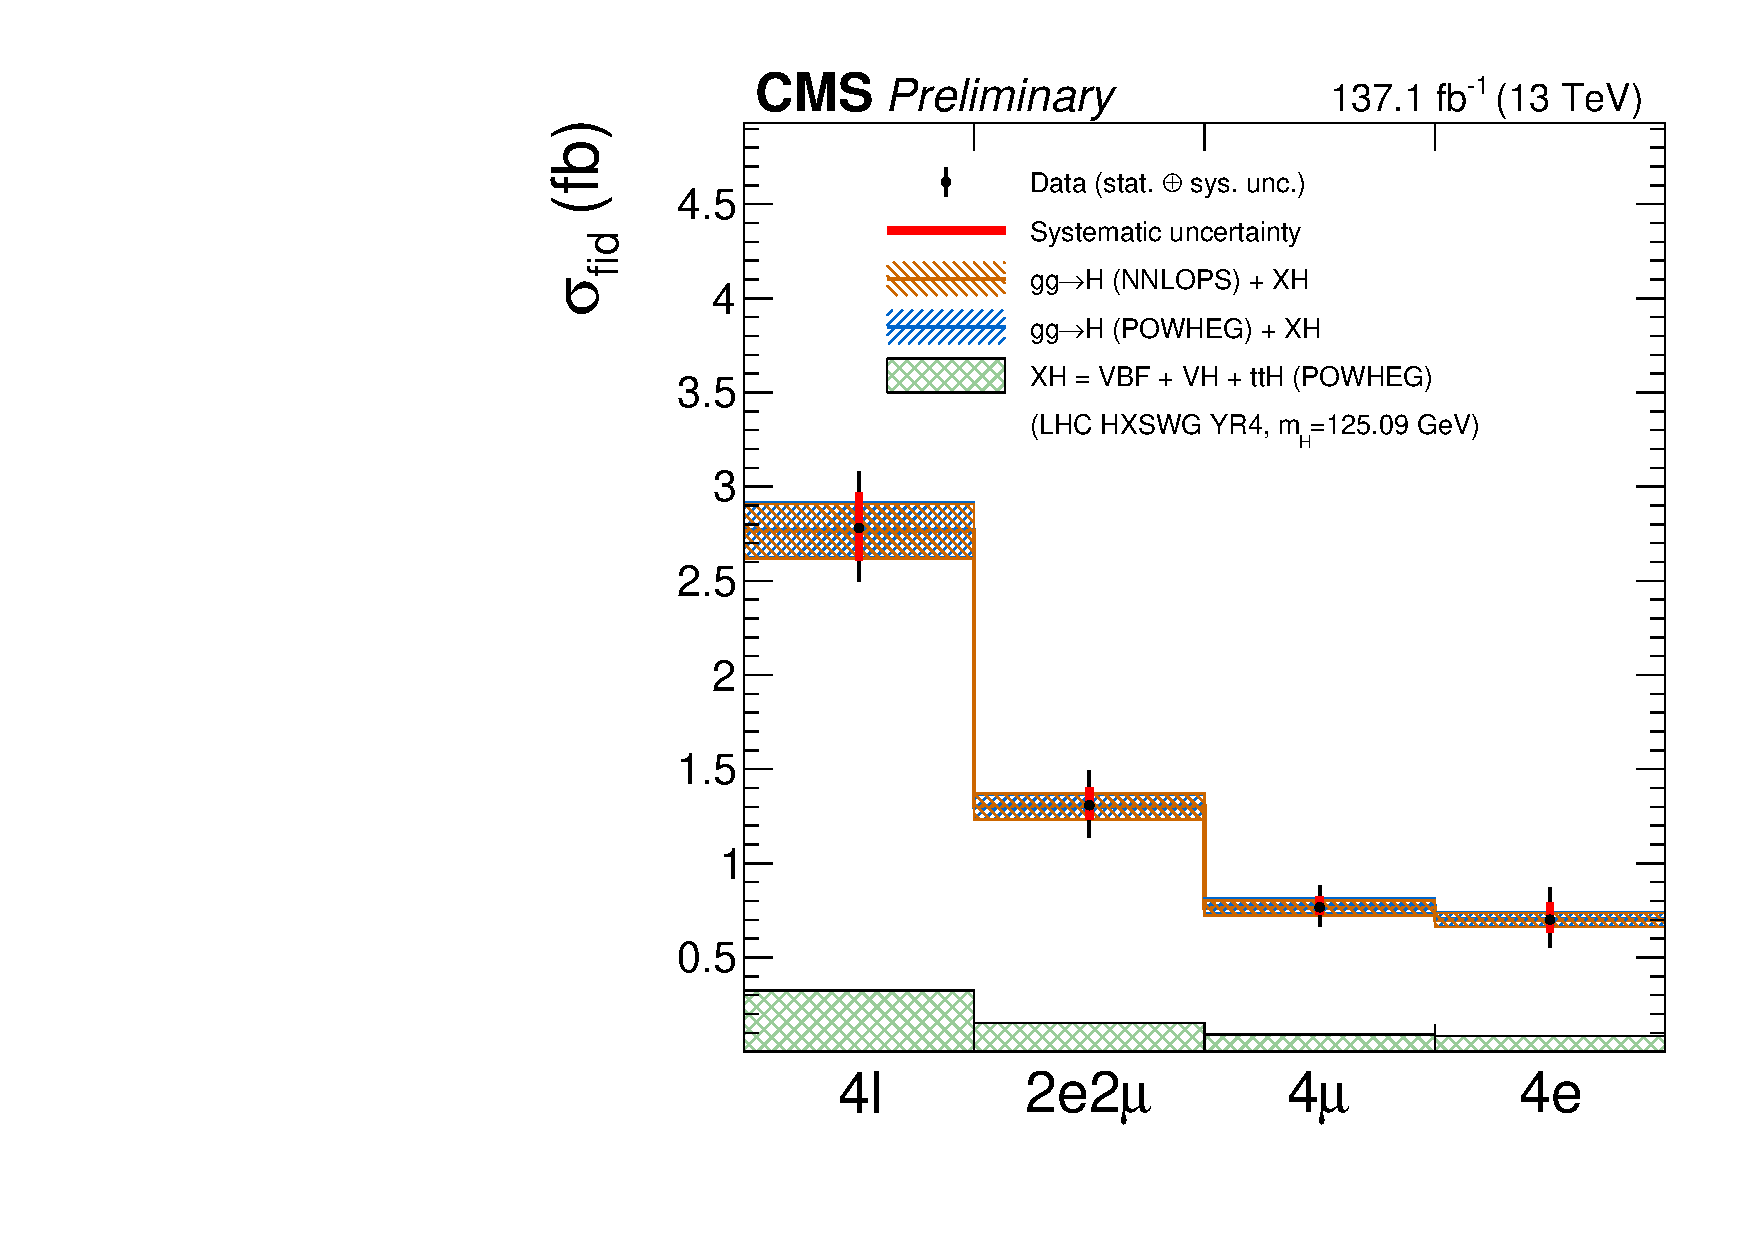
\includegraphics[width=0.45\linewidth]{Figures/results/fiducial/comb/mass4l_unfoldwith_SM_125.pdf}
%        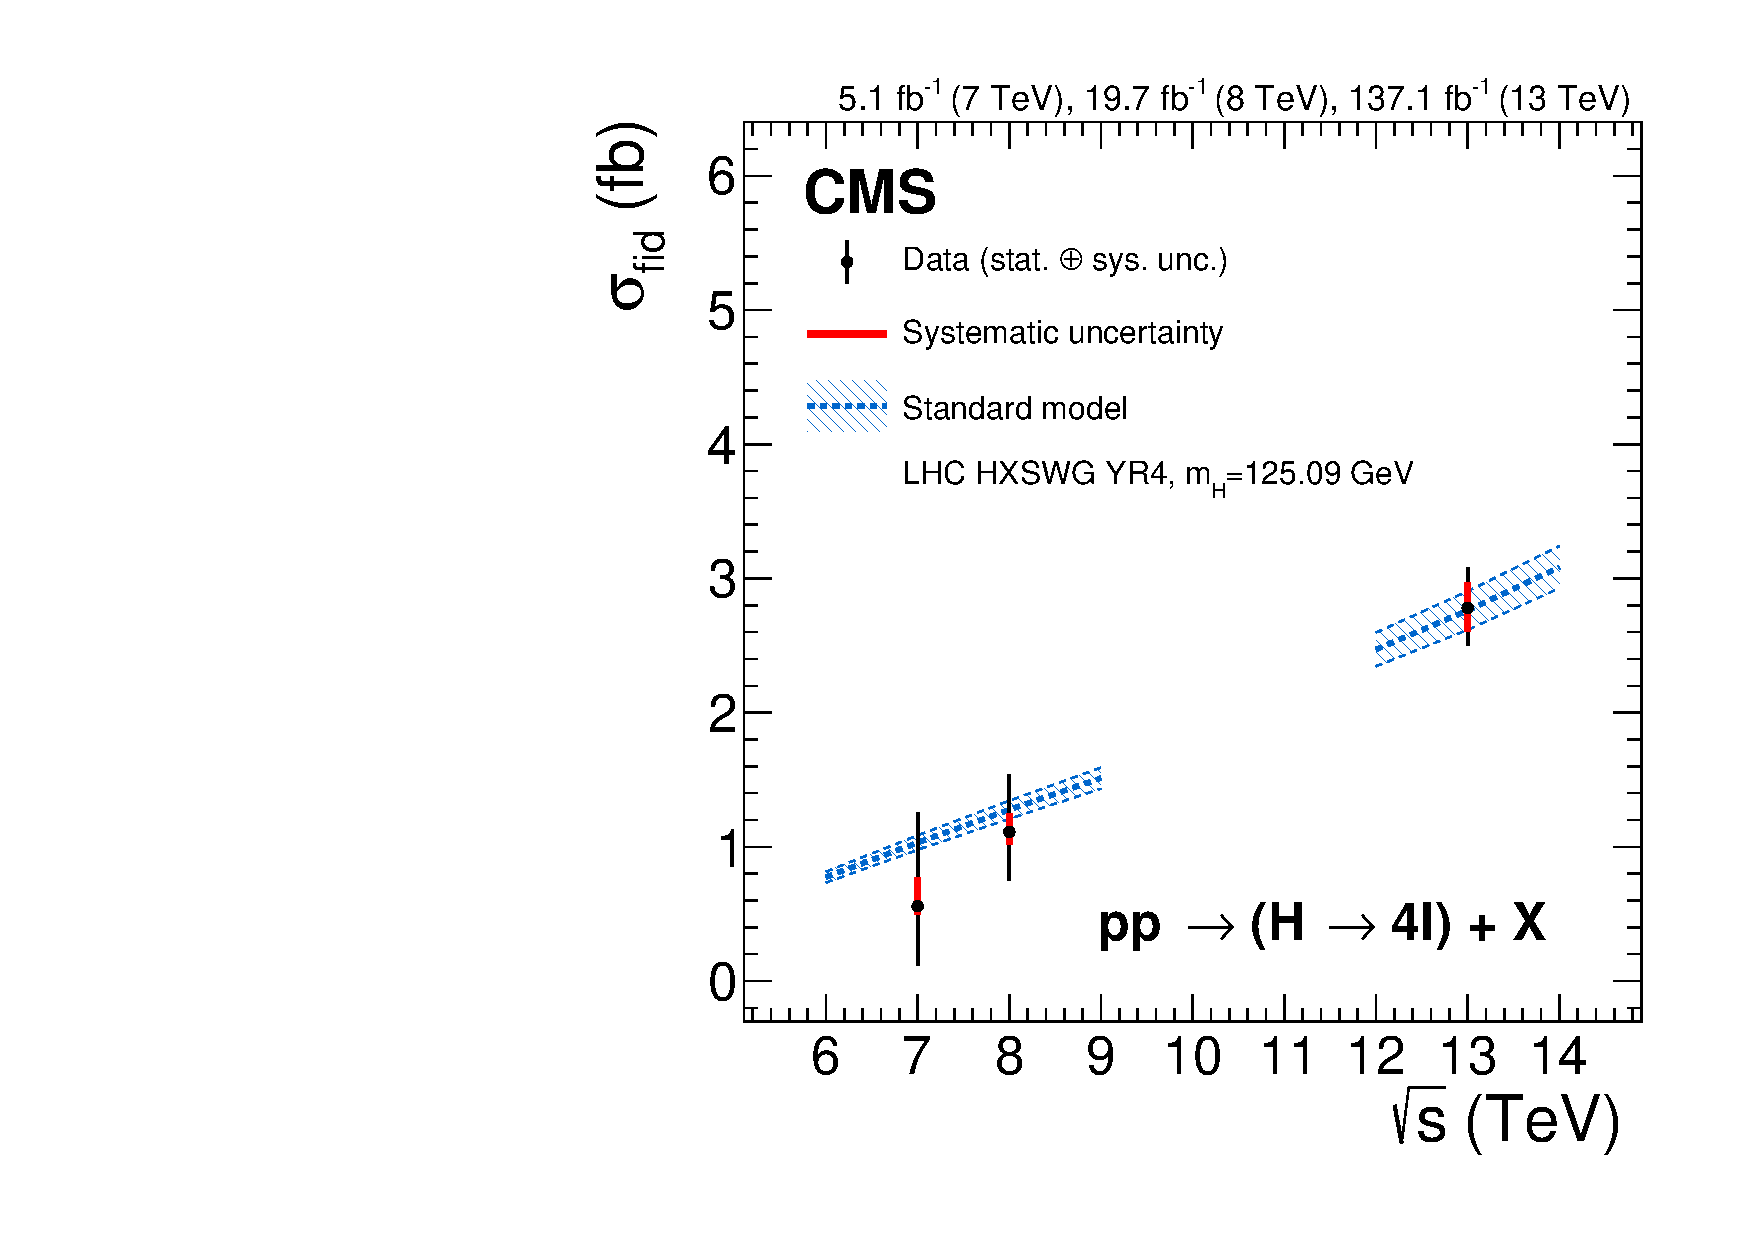
\includegraphics[width=0.45\linewidth]{Figures/results/fiducial/comb/xs_vs_sqrts.pdf} \\
%        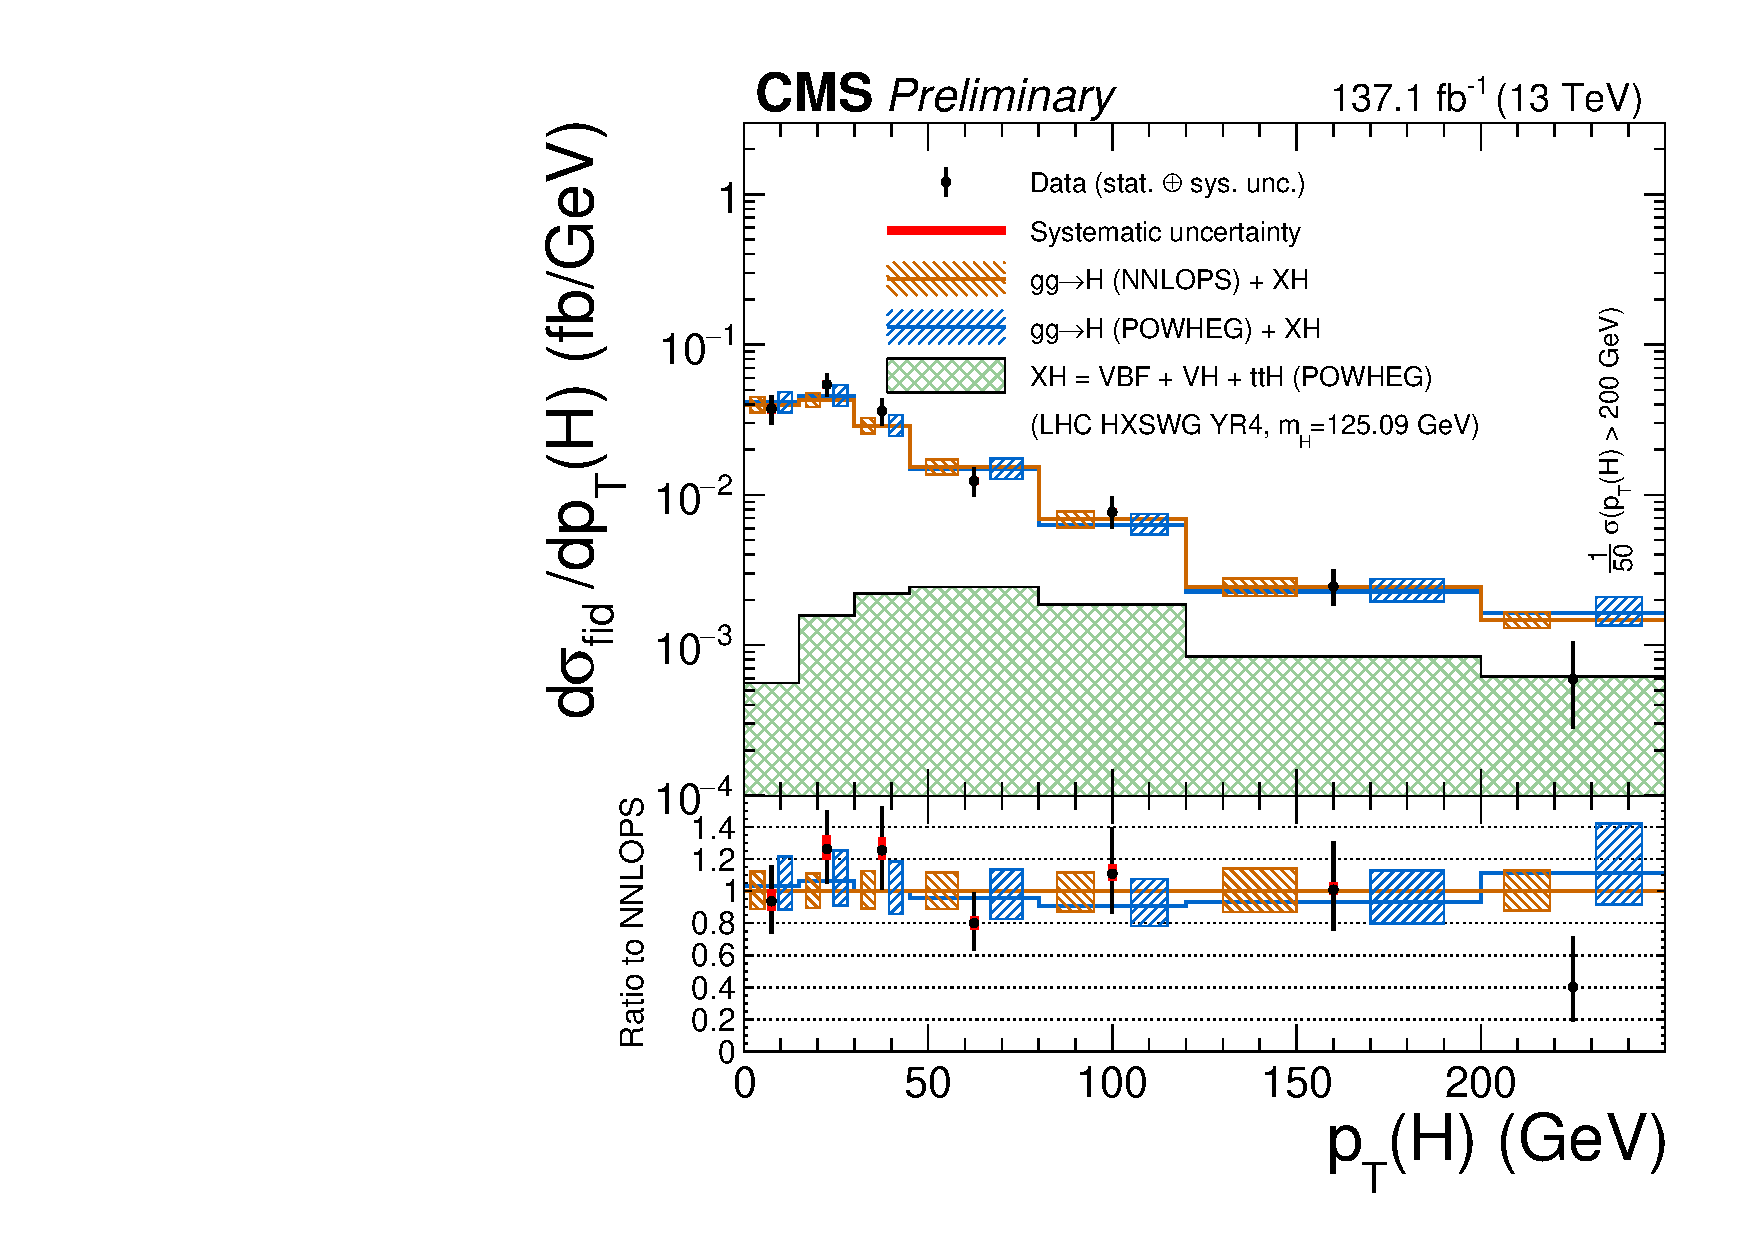
\includegraphics[width=0.45\linewidth]{Figures/results/fiducial/comb/pT4l_unfoldwith_SM_125_logscale.pdf}
%        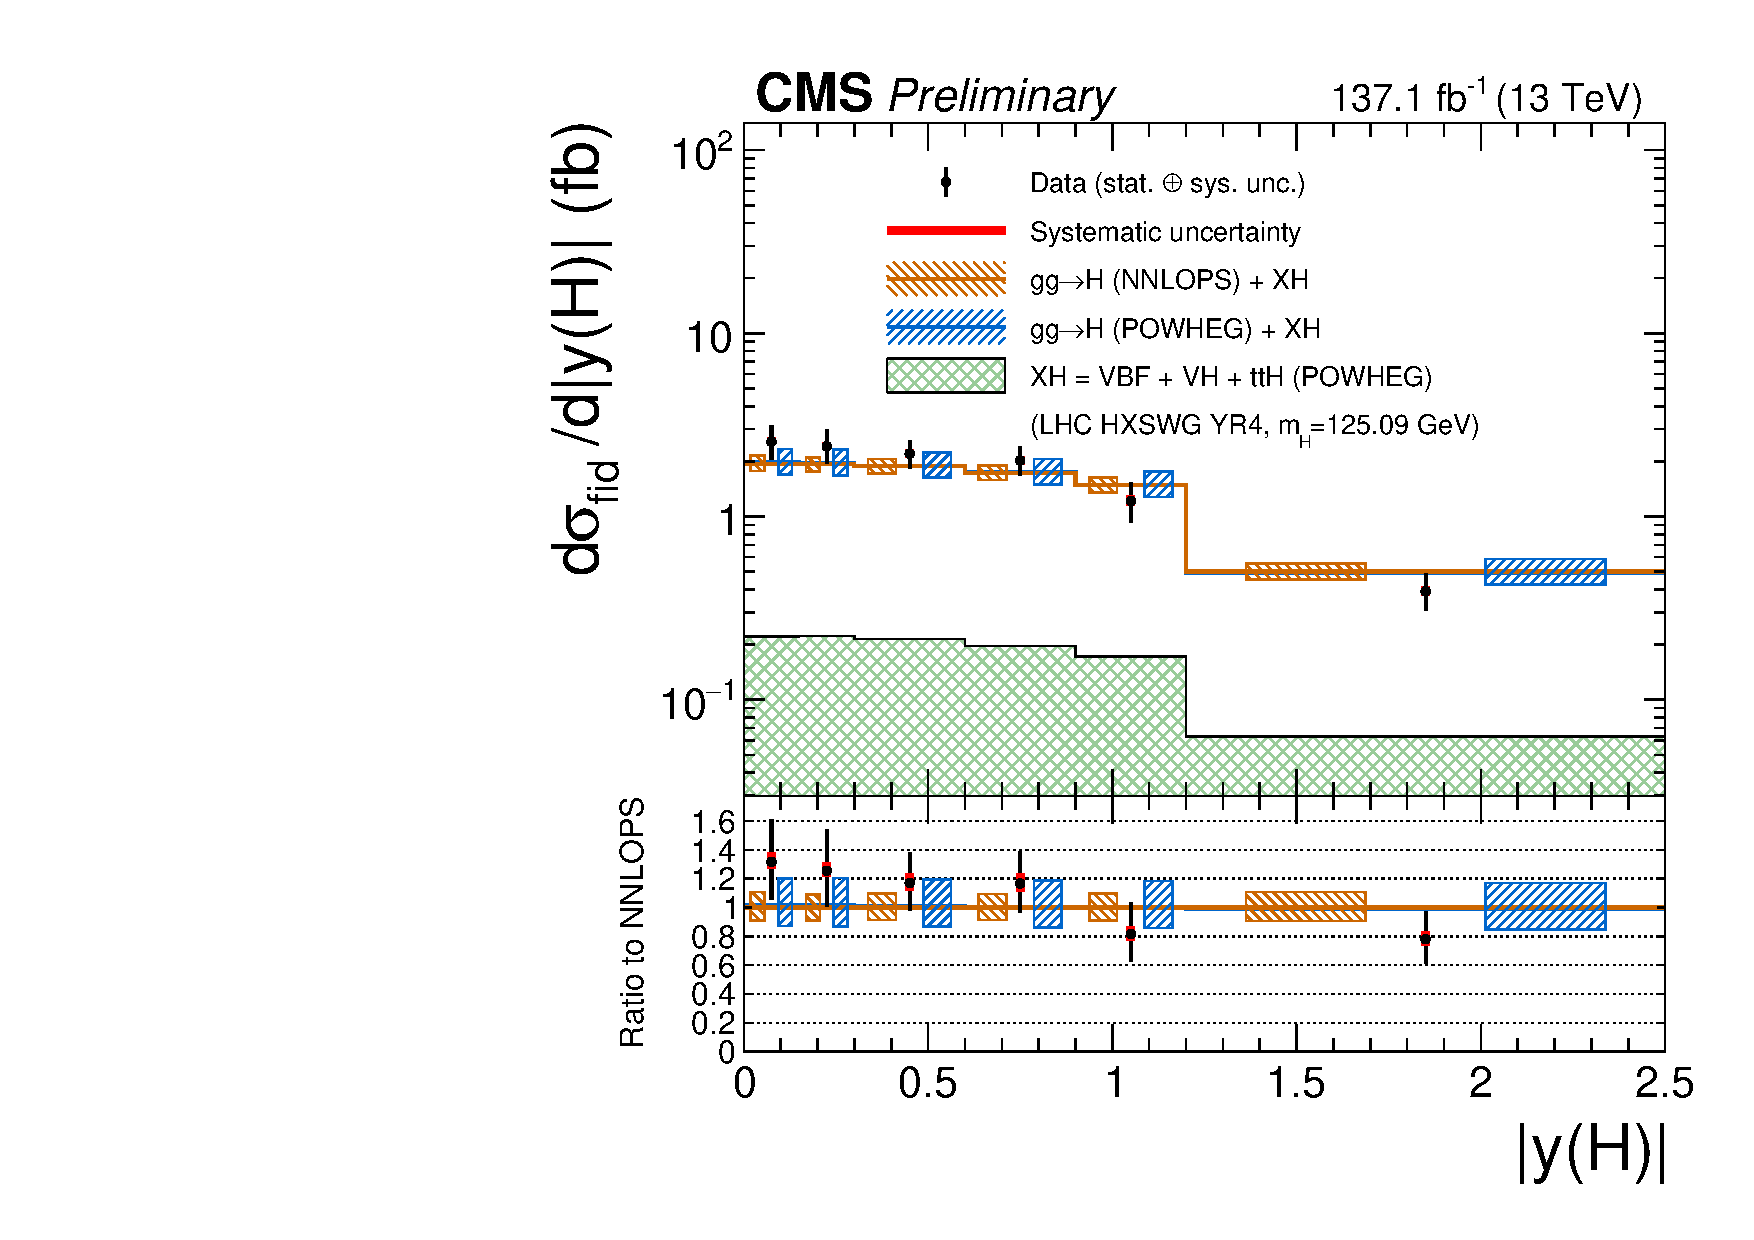
\includegraphics[width=0.45\linewidth]{Figures/results/fiducial/comb/rapidity4l_unfoldwith_SM_125_logscale.pdf} \\
%        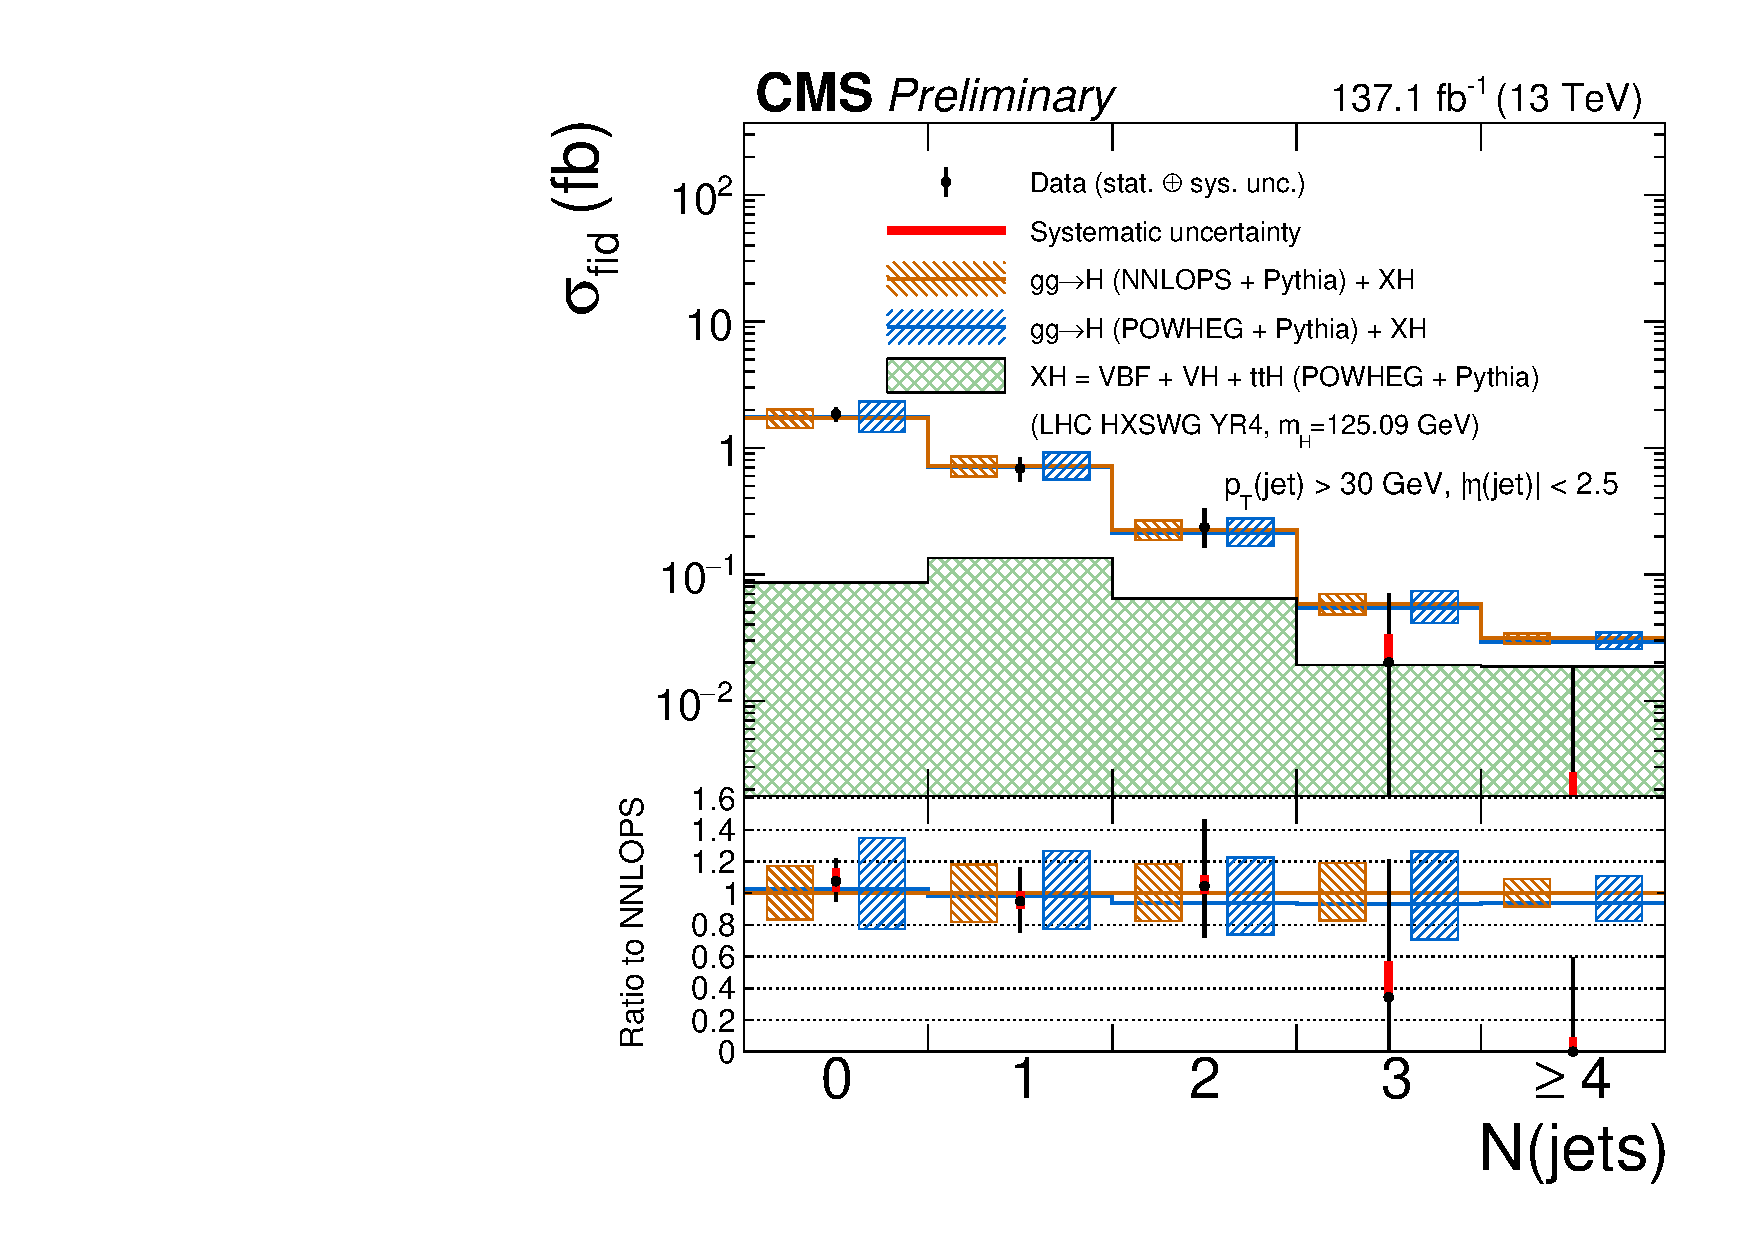
\includegraphics[width=0.45\linewidth]{Figures/results/fiducial/comb/njets_pt30_eta2p5_unfoldwith_SM_125_logscale.pdf}
%        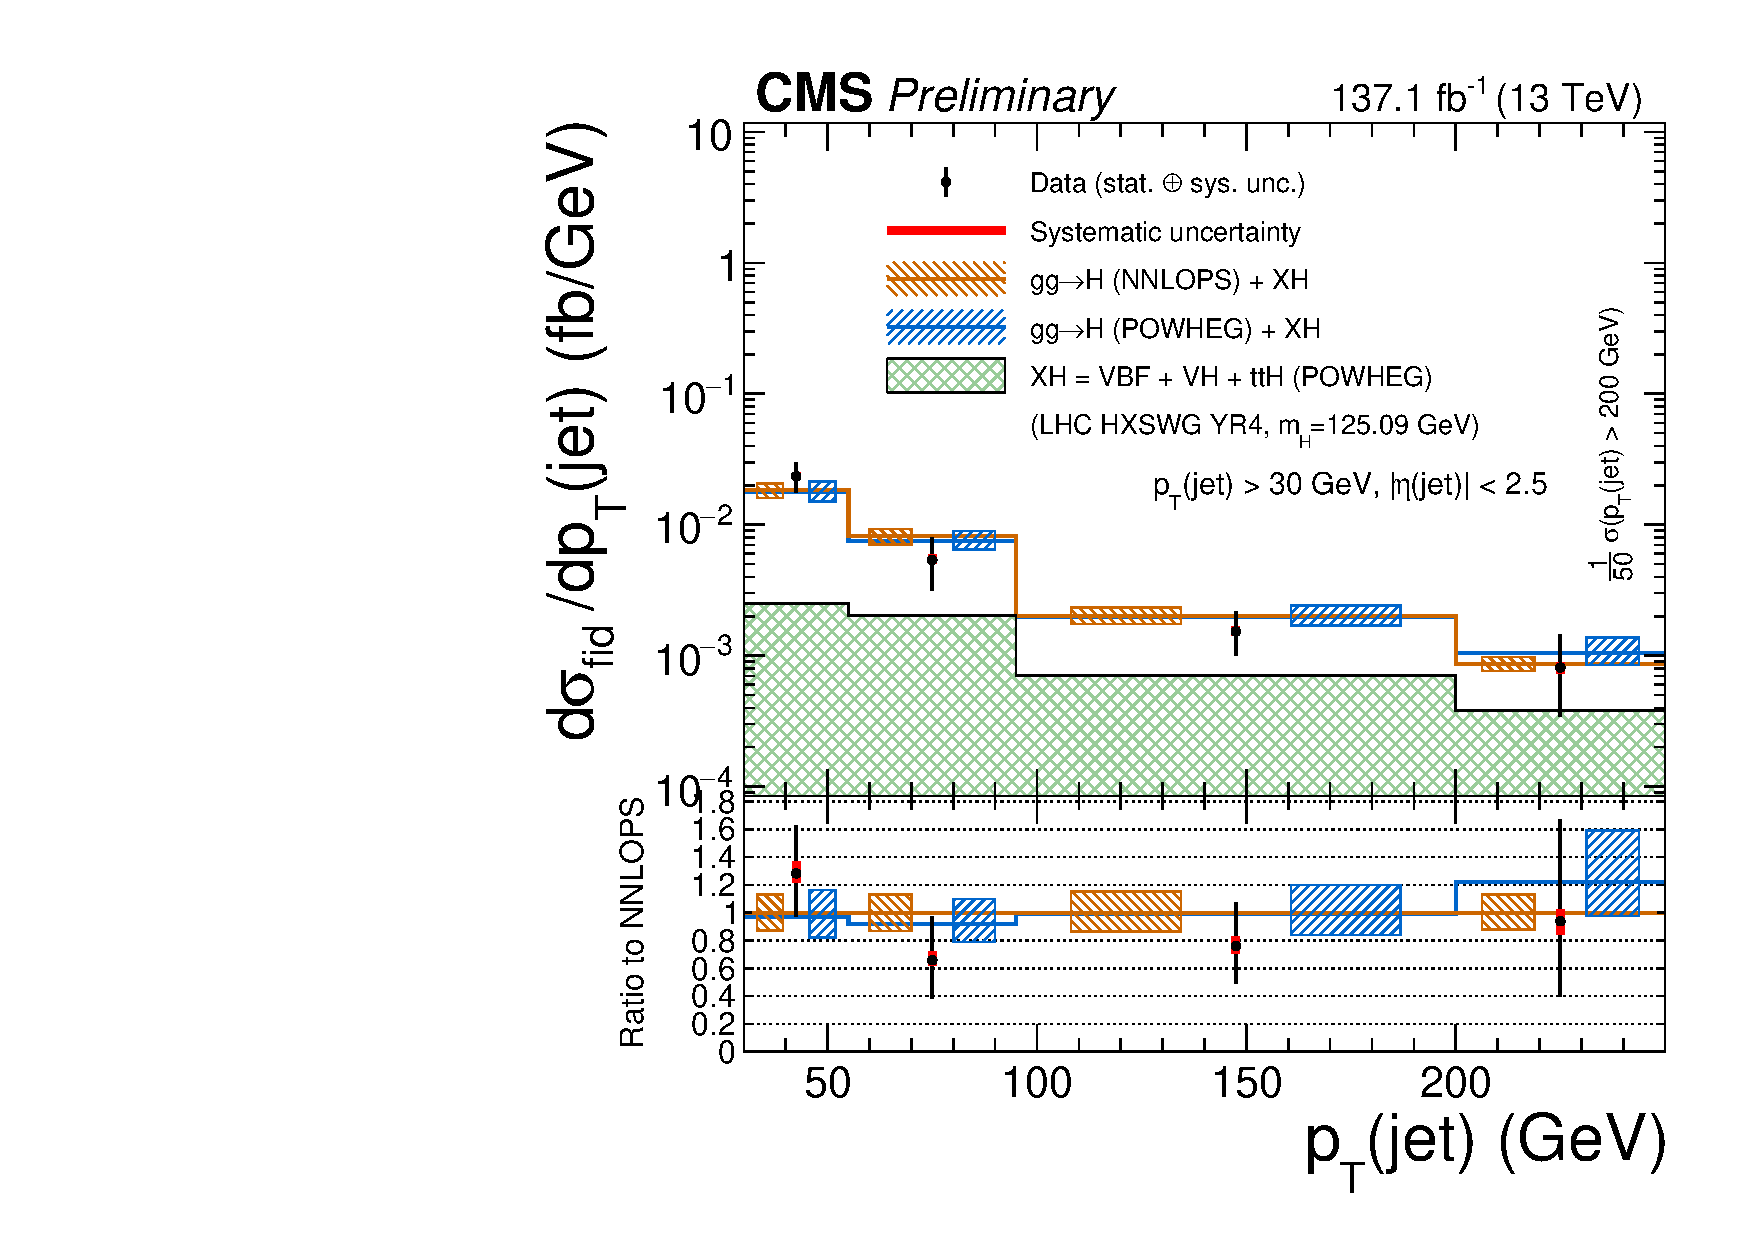
\includegraphics[width=0.45\linewidth]{Figures/results/fiducial/comb/pt_leadingjet_pt30_eta2p5_unfoldwith_SM_125_logscale.pdf}
%        \caption{
%            The measured inclusive fiducial cross subsection in different final states (top left). The measured fiducial cross subsection as a function of $\sqrt{s}$ (top right).  
%                The acceptance is calculated using \POWHEG at  $\sqrt{s}$=13\TeV and {\sc HRes}~\cite{Grazzini:2013mca,deFlorian:2012mx} 
%                at  $\sqrt{s}$=7 and 8\TeV and the total gluon fusion cross subsection and uncertainty are taken from 
%                Ref.~\cite{Anastasiou2016}. The fiducial volume for $\sqrt{s}$=6--9\TeV uses the lepton isolation definition from 
%                Ref.~\cite{CMSH4lFiducial8TeV}, while for $\sqrt{s}$=12--14\TeV the definition described in the text is used.
%                The results of the differential cross subsection measurement for $\pt({\rm H})$ (middle left), $|y({\rm H})|$ (middle right) and N(jets) (bottom left), $p_T$ of the leading jet (bottom right). The acceptance and theoreti
%cal uncertainties in the differential bins are are calculated using \POWHEG. 
%                The sub-dominant component of the the signal (VBF $+$ VH $+~\ttH$) is denoted as XH. 
%                \label{fig:fiducialresult}}
%\end{figure}
%
%
%
